% !TeX root = main.tex
% =====================================================================
%  WZL thesis (official WZLTemplate class).
%  Engine: XeLaTeX (--shell-escape).  Bibliography backend: biber.
%  Build:  latexmk  (uses .latexmkrc -> xelatex)  or  see README.
% =====================================================================
\documentclass[
    a4paper,        % a4paper/a5paper
    11pt,           % 11pt for A4, 8pt for A5
    en,             % Language [DE|EN]
    usefiramath,    % use fira math for equations
    sans,           % Font without serif (like Arial),
    % twoside,
    openright
    ]{format/WZLTemplate}


% ---------------------------------------------------------------------
%  Title metadata  (TODO: verify author, chair, supervisor, examiners)
% ---------------------------------------------------------------------
\title{Integration and Validation of Whole-Body Model Predictive Control
  for a Mobile Manipulator in Line-less Assembly}
% German translation of the title (shown in grey under the English one)
\newcommand\titlegerman{Integration und Validierung einer
  ganzk\"orperbasierten modellpr\"adiktiven Regelung f\"ur einen mobilen
  Manipulator in der linienlosen Montage}
\author{Xiangming You}                 % TODO: fill in your full name
\date{\today}                          % or \formatdate{dd}{mm}{yyyy}

% Thesis type: PA (Projektarbeit / Project Thesis)
\newcommand{\thesistype}{PA}           % options: PA, BA, MA, Dissertation
\newcommand\studentid{Matriculation No.~440593}   % TODO: fill in your student ID
\newcommand\institute{Chair of Intelligence in Quality Sensing | WZL |
  RWTH Aachen University}                     % TODO: verify chair
\newcommand\institutegerman{Lehrstuhl f\"ur Informations-, Qualit\"ats-
  und Sensorsysteme in der Produktion | WZL | RWTH Aachen}   % TODO: verify
\newcommand\supervisor{Guillaume Tréheux, M.Sc.}
\newcommand\firstexaminer{Univ.-Prof. Dr.-Ing. Robert H. Schmitt}  % TODO: verify
\newcommand\secondexaminer{}                  % add if applicable


% Set up Bibliography (biblatex + biber). Two resources, split by whether a
% reference manager can own the entry -- see lit/README.md.
%   References.bib      published literature, Crossref-verified
%   sources-manual.bib  repos, vendor docs, standards, manuals, internal reports
\bibliography{lit/References.bib}
\addbibresource{lit/sources-manual.bib}

% Set up Graphics
\graphicspath{{./03_figures/}}

%% Import Custom Packages (siunitx, cleveref, ...)
% !TeX root = ../main.tex
% Custom packages added on top of the WZL class.
% NOTE: the class already loads graphicx, caption, subcaption, booktabs,
% tabularx, float, amsmath, amssymb, bm, xcolor, hyperref, biblatex,
% csquotes, microtype, unicode-math (Fira Math). Do NOT reload those.

% --- Units & numbers -------------------------------------------------
\usepackage{siunitx}
\sisetup{detect-all, per-mode=symbol, group-separator={,}}
\DeclareSIUnit{\hz}{Hz}

% --- Clever cross-references (load AFTER hyperref, which the class does)
\usepackage[capitalise,noabbrev]{cleveref}

% --- TikZ libraries for the architecture diagrams --------------------
% (tikz itself arrives with todonotes, loaded by the class)
\usepackage{tikz}
\usetikzlibrary{arrows.meta, positioning, fit, calc}
\usepackage{pgfplots}
\pgfplotsset{
  compat=1.18,
  every axis/.append style={
    font=\footnotesize,
    grid=major,
    grid style={dotted, gray!40},
    tick label style={font=\scriptsize},
    legend style={font=\scriptsize, draw=none, fill=none, row sep=1pt},
  },
}

% --- Draft watermark (uncomment while drafting) ----------------------
% \usepackage{draftwatermark}


% Begin of the document
\begin{document}

%% Define own commands (\ocs, \mpc, \hero, \ee, math vectors, ...)
% !TeX root = ../main.tex
%% Custom commands used throughout the thesis.

% --- Handy text macros -----------------------------------------------
\newcommand{\ocs}{OCS2}
\newcommand{\mpc}{MPC}
\newcommand{\ee}{end-effector}
\newcommand{\EE}{End-effector}
\newcommand{\hero}{HERo}

% --- Math: state / input vectors -------------------------------------
% \symbf (unicode-math) rather than \bm: the class loads unicode-math with
% Fira Math, where \bm produces extended mathchars that XeTeX rejects in
% sub/superscript and accent positions.
\newcommand{\svec}{\symbf{x}}
\newcommand{\uvec}{\symbf{u}}
\newcommand{\qarm}{\symbf{q}_{\mathrm{arm}}}
\newcommand{\qarmdot}{\dot{\symbf{q}}_{\mathrm{arm}}}


%% Set up keyphrases
% !TeX root = main.tex

% Enter your recurring Keyphrases like research questions here

%%%%% ----- 
%%%%% ----- FORSCHUNGSFRAGEN -----
%%%%% ----- 

\newcommand{\Hauptforschungsfrage}{?}



% Titlepage
\makeatletter

% Define academic degree names based on the thesis type
\ifthenelse{\equal{\thesistype}{Dissertation}}{%
    \def\academicdegree{Dissertation}%
    \def\academicdegreegerman{Dissertation}%
}{%
    \ifthenelse{\equal{\thesistype}{PA}}{%
        \def\academicdegree{Project Thesis}%
        \def\academicdegreegerman{Projektarbeit}%
    }{%
        \ifthenelse{\equal{\thesistype}{BA}}{%
            \def\academicdegree{Bachelor Thesis}%
            \def\academicdegreegerman{Bachelorarbeit}%
        }{%
            \ifthenelse{\equal{\thesistype}{MA}}{%
                \def\academicdegree{Master Thesis}%
                \def\academicdegreegerman{Masterarbeit}%
            }{%
                % Default case
                \def\academicdegree{Thesis}%
                \def\academicdegreegerman{Arbeit}%
            }}}}

\begin{titlepage}

    % Temporarily adjust the page margins to increase the usable space
    % \newgeometry{top=2cm,bottom=2cm,left=2cm,right=2cm}

    \ifnum\papersize=4
        \begin{tikzpicture}[remember picture,overlay]
            \node[opacity=0.4, anchor=north east,inner sep=0pt]%
            at ($(current page.north west)+(20.5cm,-0.5cm)$)
            {
\includegraphics[width=7.67cm]{wzl_eps_hks44.pdf}};
        \end{tikzpicture}
    \else
        \begin{tikzpicture}[remember picture,overlay]
            \node[opacity=0.4, anchor=north east]%
            at (current page.north east)%
            {
\includegraphics[width=5.4cm]{wzl_eps_hks44.pdf}};
        \end{tikzpicture}
    \fi

    \begin{flushleft}
        {\small
        The present work was submitted to the \\ \institute.\\
        {\color{black!50} Diese Arbeit wurde vorgelegt am \institutegerman.}
        }

        \vfill

        \textbf{\Large\@title}

        \textbf{\Large\color{black!50}\titlegerman}

    \end{flushleft}

    \vspace{1cm}

    \textbf{\large\academicdegree\color{black!50}\ /\ \academicdegreegerman }

    \vfill

    \textbf{\color{black!75}Presented by\color{black!50}\ /\ Vorgelegt von}

    {\@author}\\
    \studentid
    \vfill
    % Supervisor and Examiners
    {
        \textbf{\color{black!75}Supervised by\color{black!50}\ /\ Betreut von} \supervisor
        \\
        \textbf{\color{black!75}\\1\textsuperscript{st} Examiner\color{black!50}\ /\ 1. Prüfer} \firstexaminer
        % Include 2nd examiner only if it's set
        \ifthenelse{\equal{\secondexaminer}{}}{}{%
            \\
            \textbf{\color{black75}\\2\textsuperscript{nd} Examiner\color{black!50}\ /\ 2. Prüfer} \secondexaminer
        }
    }

    \begin{flushright}
        {\small
            Aachen, \@date
        }
    \end{flushright}

    \vfill

    % Include the disclaimer text on the title page if applicable
    \ifthenelse{\equal{\thesistype}{Dissertation}}{}{%
        % Reduce vertical space before the disclaimer
        \vspace{0.5cm}
        \noindent {\footnotesize
            Inhalt und Ergebnis dieser Arbeit sind ausschließlich zum internen Gebrauch bestimmt. Alle Urheberrechte liegen bei der RWTH Aachen. Ohne ausdrückliche Genehmigung des betreuenden Lehrstuhls ist es nicht gestattet, diese Arbeit oder Teile daraus an Dritte weiterzugeben.

            \medskip

            \textit{The content and results of this thesis are intended exclusively for internal use. All copyrights are held by RWTH Aachen University. Without the express permission of the supervising department, it is not permitted to pass this thesis or parts thereof to third parties.}
        }
    }

    % Reset page geometry back to normal
    \restoregeometry

\end{titlepage}


\makeatother

\newpage\thispagestyle{empty}\null

% -- FRONTMATTER --
\include{frontmatter}


% -- CHAPTERS --
% !TeX root = ../main.tex
\chapter{Introduction to Line-less Mobile Assembly Systems}
\label{ch:introduction}

% =====================================================================
\section{Line-less Mobile Assembly Systems and Their Implications for
  Motion Planning}
\label{sec:lmas}

Manufacturing operates under shortening product life cycles, growing
variant diversity, and demand that fluctuates over the life of a
product; a CIRP-level review of product-variety management documents
this trend across industries and quantifies the cost it imposes on
assembly~\cite{ElMaraghy2013Variety}. Rigid, station-based assembly
lines are dimensioned for a fixed product mix and a stable takt time.
When the product or the required volume changes, layout, material flow,
and station balancing have to be reconfigured, which is slow and
capital-intensive~\cite{Huettemann2016LMAS}.

Manufacturing research has answered this tension with a family of
paradigms that trade dedicated throughput for adaptability. Flexible
Manufacturing Systems provide a fixed set of capabilities that can be
re-combined for a pre-defined product family, whereas Reconfigurable
Manufacturing Systems are designed so that capacity and functionality
themselves can be changed by adding, removing, or rearranging
modules~\cite{Koren1999RMS}. ElMaraghy contrasts the two paradigms and
places them on a common axis of changeability, with flexibility bought
in advance in the former case and acquired on demand in the
latter~\cite{ElMaraghy2005FRMS}. In assembly specifically, this line of
work has produced modular station concepts in which workstations are no
longer traversed in a fixed sequence~\cite{Kern2016Modular}.

The \emph{Line-less Mobile Assembly System} (LMAS) pushes this
development to its limit by removing the fixed station grid
altogether~\cite{Huettemann2019LMAS}. Instead of binding products,
tools, and workers to a sequence of static stations, an LMAS models all
production resources---mobile robots, mobile manipulators, workpiece
carriers, and human workers---as \emph{mobile, freely relocatable
entities} on a shared shop floor, whose assignment, sequence, and
location are planned at run time~\cite{Buckhorst2019Planning}. The
assembly ``line'' thus becomes a reconfigurable constellation of
resources matched to the current order, and control of that
constellation is decentralised so that the system can absorb product
changes, demand fluctuations, and disturbances without a physical
relayout~\cite{Buckhorst2022LMAS}.

A central enabler of the LMAS concept is the \emph{mobile manipulator}:
a robotic arm mounted on a mobile base
(\cref{fig:mobile-manipulator}). The mobile base extends the reachable
workspace far beyond the arm's own envelope and lets the robot
reposition itself between and within tasks, while the arm provides the
dexterity required for the assembly operation itself. Surveys of the
field identify exactly this combination (one resource servicing many
workstations, covering workpieces larger than a fixed-base arm could
reach) as the motivation for wheeled mobile
manipulation~\cite{Sandakalum2022Survey,Thakar2023MobileManip}.

\begin{figure}[htbp]
  \centering
  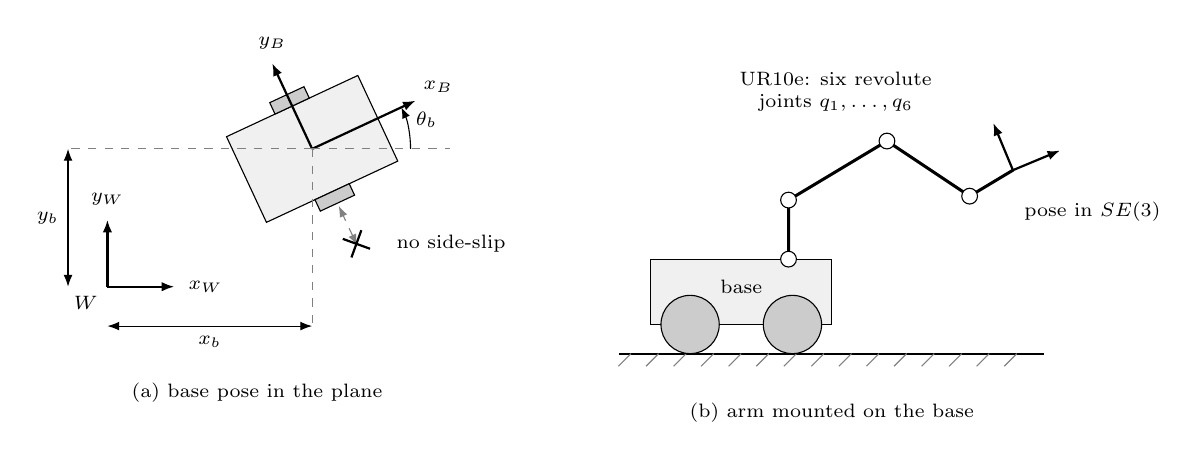
\begin{tikzpicture}[
      font=\footnotesize,
      lbl/.style={font=\scriptsize, align=center},
      dim/.style={{Latex[length=1.5mm]}-{Latex[length=1.5mm]}, thin},
      link/.style={line width=1.1pt, line cap=round},
      jt/.style={circle, draw, fill=white, inner sep=0pt, minimum size=2.0mm},
      ax/.style={-{Latex[length=1.6mm]}, thick},
    ]
    % =================================================================
    % (a) top view: planar base pose and the no-slip direction
    % =================================================================
    \begin{scope}[shift={(0,0)}]
      \draw[ax] (0,0) -- (0.85,0) node[lbl, right=0.5mm] {$x_W$};
      \draw[ax] (0,0) -- (0,0.85) node[lbl, above=0.5mm] {$y_W$};
      \node[lbl, below left=0mm] at (0,0) {$W$};

      \begin{scope}[shift={(2.6,1.75)}, rotate=25]
        \draw[fill=gray!12] (-0.92,-0.60) rectangle (0.92,0.60);
        \draw[fill=gray!40] (-0.24,-0.60) rectangle (0.24,-0.76);
        \draw[fill=gray!40] (-0.24, 0.60) rectangle (0.24, 0.76);
        \draw[ax] (0,0) -- (1.45,0) node[lbl, above right=-0.4mm] {$x_B$};
        \draw[ax] (0,0) -- (0,1.20) node[lbl, above=0.5mm] {$y_B$};
        % blocked lateral direction
        \draw[dashed, gray, {Latex[length=1.4mm]}-{Latex[length=1.4mm]}]
          (0,-1.35) -- (0,-0.80);
        \draw[thick] (-0.13,-1.20) -- (0.13,-1.46);
        \draw[thick] (-0.13,-1.46) -- (0.13,-1.20);
      \end{scope}
      \node[lbl, anchor=west] at (3.55,0.55) {no side-slip};

      \draw[dim] (0,-0.50) -- (2.6,-0.50) node[lbl, midway, below] {$x_b$};
      \draw[dim] (-0.50,0) -- (-0.50,1.75) node[lbl, midway, left] {$y_b$};
      \draw[dashed, gray] (2.6,1.75) -- (2.6,-0.50);
      \draw[dashed, gray] (2.6,1.75) -- (-0.50,1.75);
      \draw[dashed, gray] (2.6,1.75) -- ++(1.75,0);
      \draw[-{Latex[length=1.4mm]}] (3.85,1.75) arc (0:25:1.25);
      \node[lbl] at (4.05,2.12) {$\theta_b$};

      \node[lbl, anchor=north] at (1.9,-1.10) {(a) base pose in the plane};
    \end{scope}

    % =================================================================
    % (b) side view: base plus six-joint arm
    % =================================================================
    \begin{scope}[shift={(6.9,-0.60)}]
      \draw[thick] (-0.4,-0.25) -- (5.0,-0.25);
      \foreach \x in {-0.25,0.10,...,4.90}
        \draw[gray, thin] (\x,-0.25) -- ++(-0.16,-0.16);

      \draw[fill=gray!12] (0.0,0.12) rectangle (2.3,0.95);
      \draw[fill=gray!40] (0.5,0.12) circle (0.37);
      \draw[fill=gray!40] (1.8,0.12) circle (0.37);
      \node[lbl] at (1.15,0.60) {base};

      \coordinate (a0) at (1.75,0.95);
      \coordinate (a1) at (1.75,1.70);
      \coordinate (a2) at (3.00,2.45);
      \coordinate (a3) at (4.05,1.75);
      \coordinate (a4) at (4.60,2.08);
      \draw[link] (a0) -- (a1) -- (a2) -- (a3) -- (a4);
      \node[jt] at (a0) {}; \node[jt] at (a1) {};
      \node[jt] at (a2) {}; \node[jt] at (a3) {};
      \node[lbl, anchor=south] at (2.35,2.70)
        {UR10e: six revolute\\joints $q_1,\dots,q_6$};

      \draw[ax] (a4) -- ++(0.60,0.25);
      \draw[ax] (a4) -- ++(-0.25,0.60);
      \node[lbl, anchor=north west] at (4.62,1.90) {\ee{}\\pose in $SE(3)$};

      \node[lbl, anchor=north] at (2.3,-0.75) {(b) arm mounted on the base};
    \end{scope}
  \end{tikzpicture}
  \caption[Mobile manipulator: base and arm degrees of freedom]{%
    Wheeled mobile manipulator of the type studied here. (a)~The base
    contributes the planar pose $(x_b,y_b,\theta_b)$; its wheels cannot
    slide sideways, which constrains the velocities it can produce but
    not the poses it can reach. (b)~The arm contributes six revolute
    joints, and the task is the pose of the \ee{} frame in $SE(3)$.
    Counting these groups against the task is what makes the system
    redundant (\cref{eq:grubler,eq:redundancy}).}
  \label{fig:mobile-manipulator}
\end{figure}

Adding a mobile base to the arm changes the motion-planning problem in
three ways. In a classical line, an industrial arm operates in an
engineered, static cell: the part arrives at a known pose, the
surroundings are fixed, and the arm executes largely pre-programmed
trajectories. In an LMAS, three of the assumptions behind that mode of
operation are weakened.

\paragraph{Large, base-dependent workspace.}
The target \ee{} pose may lie outside the reach of the arm from the
current base pose, so base and arm have to \emph{cooperate} to
accomplish a single task. Both mobile-manipulation surveys treat the
choice of a base pose that renders the task reachable and
well-conditioned as a planning problem in its own
right~\cite{Sandakalum2022Survey,Thakar2023MobileManip}.

\paragraph{Shared workspace with moving resources.}
Because resources are relocatable, parts of the environment move
relative to one another during operation. How much of the environment is
known in advance depends on the plant: a shop floor with tracked
resources and a maintained world model is partially predictable, whereas
human co-workers and manually moved carriers are not. The consequence
for planning is therefore not that offline computation is impossible,
but that a trajectory computed once for an assumed scene has to be
revised while it is executed, which is the case that motivates online
re-planning~\cite{Finean2023ContextAware}.

\paragraph{Kinematic redundancy.}
The base adds degrees of freedom (DOF) to a system that already has as
many as the task requires. The arm is a spatial open chain with
$N = 7$ links (including its mounting link) connected by $J = 6$
revolute joints, each contributing $f_i = 1$ freedom. Gr\"ubler's
formula for a spatial mechanism ($m = 6$) gives its
mobility~\cite{Lynch2017ModernRobotics}
\begin{equation}
  \label{eq:grubler}
  \mathrm{dof} = m\,(N - 1 - J) + \sum_{i=1}^{J} f_i
               = 6\,(7 - 1 - 6) + 6 = 6 .
\end{equation}
The base contributes a planar pose, so the whole-body configuration is
$q = (x_b, y_b, \theta_b, q_1, \dots, q_6)$ and the configuration space
is nine-dimensional, while the \ee{}-pose task lives in the
six-dimensional $SE(3)$:
\begin{equation}
  \label{eq:redundancy}
  \dim \mathcal{Q} - \dim \mathcal{T} = 9 - 6 = 3 .
\end{equation}
Three configuration-space directions therefore leave the \ee{} pose
unchanged. The picture differs at velocity level, because a
differential-drive base cannot slide sideways: the rolling-without-slip
condition $\dot{x}_b \sin\theta_b - \dot{y}_b \cos\theta_b = 0$ is a
non-holonomic constraint, so the base offers only two instantaneous
inputs (a forward and a turning rate) while still reaching all three
planar coordinates over time~\cite{Lynch2017ModernRobotics,%
Siciliano2009Robotics}. The instantaneous input vector is therefore
eight-dimensional against a six-dimensional task twist, leaving two
degrees of instantaneous redundancy. This redundancy is an opportunity:
the same \ee{} motion can be produced by infinitely many base--arm
combinations, and the surplus can be spent on reach, on
manipulability~\cite{Yoshikawa1985Manipulability}, or on obstacle
avoidance~\cite{Dietrich2015NullSpace}. It is an opportunity only if the
planner reasons about base and arm \emph{jointly}; a planner that fixes
the base first spends the redundancy before it can be used.

Together, these three conditions call for motion planning that is
reactive, that spans the \emph{combined} configuration space of base and
arm, and that resolves the resulting redundancy deliberately rather than
as a by-product. Whole-body motion planning, introduced next, addresses
exactly this problem.

% =====================================================================
\section{The Need for Whole-Body Motion Planning: From Sequential to
  Unified Approaches}
\label{sec:need-wholebody}

The most common way to command a mobile manipulator is to treat base and
arm as two independent subsystems and to plan for them
\emph{sequentially}: a navigation stack such as
Nav2~\cite{Macenski2020Nav2} first drives the base to a suitable
stand-off pose; an arm-motion framework such as
MoveIt~\cite{moveit2} then solves the inverse kinematics for the target
\ee{} pose from that now-fixed base pose and plans a joint-space
trajectory to the resulting configuration, typically with a
sampling-based planner~\cite{Sucan2012OMPL}. This decoupled scheme is
modular and, above all, built from components that are mature and
widely deployed in industry, which is the practical reason for its
prevalence; both mobile-manipulation surveys report it as the dominant
architecture in fielded
systems~\cite{Sandakalum2022Survey,Thakar2023MobileManip}.

Decoupling has three consequences that become severe in the LMAS
setting; \cref{fig:decoupled-vs-wholebody} contrasts the two schemes.

\paragraph{Loss of reach and of solution quality.}
Choosing the base pose \emph{before} planning the arm discards the
coupling between the two subsystems. A base pose that looks reasonable
geometrically may leave the arm near a singularity or a joint limit, or
may make the \ee{} target unreachable, even though a jointly chosen
base--arm configuration
exists~\cite{Sandakalum2022Survey,Thakar2023MobileManip}. Both surveys
describe base placement and arm planning as coupled sub-problems, and
the holistic controller of Haviland et~al.\ is motivated by the same
observation~\cite{Haviland2022Holistic}.

\paragraph{Stop-and-go behaviour.}
Sequential execution---drive, stop, then manipulate---prevents base and
arm from moving \emph{simultaneously}. Tasks in which the \ee{} has to
follow a continuous path longer than the arm's reach, which is a common
LMAS case, cannot be executed smoothly this
way~\cite{BurgessLimerick2024ReactiveBase,Pankert2020PerceptiveMPC}.
Reported gains of on-the-move manipulation over the stop-and-go pipeline
motivate both the reactive base controller of Burgess-Limerick
et~al.\ and the continuous mobile manipulation of Pankert and Hutter.

\paragraph{Cost of reacting to change.}
A plan computed once, for a fixed base pose, does not by itself account
for base drift, moving obstacles, or an updated target. This is a
question of degree rather than of possibility: the pipeline can be
re-triggered, and planners that predict how the scene will evolve and
repair the trajectory online exist~\cite{Finean2023ContextAware}. What a
decoupled pipeline cannot do cheaply is revise the \emph{base} decision,
because that decision sits upstream of the arm plan and invalidates it.

\begin{figure}[htbp]
  \centering
  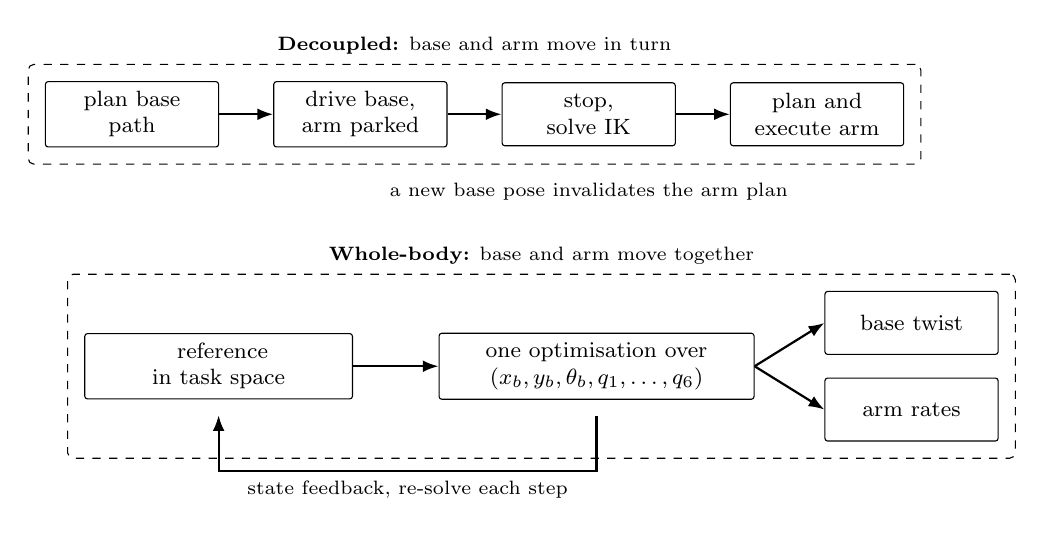
\begin{tikzpicture}[
      font=\footnotesize,
      box/.style={draw, rounded corners=1pt, align=center,
                  inner sep=3.5pt, minimum height=8mm, minimum width=22mm},
      flow/.style={-{Latex[length=2mm]}, thick},
      lbl/.style={font=\scriptsize, align=center},
      lane/.style={draw, dashed, rounded corners=2pt, inner sep=6pt},
    ]
    % ---------- decoupled lane --------------------------------------
    \node[box] (d1) at (0,0)    {plan base\\path};
    \node[box] (d2) at (2.9,0)  {drive base,\\arm parked};
    \node[box] (d3) at (5.8,0)  {stop,\\solve IK};
    \node[box] (d4) at (8.7,0)  {plan and\\execute arm};
    \draw[flow] (d1) -- (d2); \draw[flow] (d2) -- (d3);
    \draw[flow] (d3) -- (d4);
    \node[lane, fit=(d1)(d4),
          label={[lbl]above:\textbf{Decoupled:} base and arm move in turn}] {};
    \node[lbl, anchor=north] at (5.8,-0.75)
      {a new base pose invalidates the arm plan};

    % ---------- whole-body lane -------------------------------------
    \node[box, minimum width=34mm] (w1) at (1.1,-3.2)
      {\ee{} reference\\in task space};
    \node[box, minimum width=40mm] (w2) at (5.9,-3.2)
      {one optimisation over\\$(x_b,y_b,\theta_b,q_1,\dots,q_6)$};
    \node[box, minimum width=22mm] (w3a) at (9.9,-2.65) {base twist};
    \node[box, minimum width=22mm] (w3b) at (9.9,-3.75) {arm rates};
    \draw[flow] (w1) -- (w2);
    \draw[flow] (w2.east) -- (w3a.west);
    \draw[flow] (w2.east) -- (w3b.west);
    \draw[flow] ([yshift=-2mm]w2.south) -- ++(0,-0.7) -| ([yshift=-2mm]w1.south)
      node[lbl, pos=0.25, below] {state feedback, re-solve each step};
    \node[lane, fit=(w1)(w2)(w3a)(w3b),
          label={[lbl]above:\textbf{Whole-body:} base and arm move together}] {};
  \end{tikzpicture}
  \caption[Decoupled versus whole-body command of a mobile
    manipulator]{%
    Decoupled versus whole-body command of a mobile manipulator. The
    decoupled pipeline fixes the base pose upstream of the arm plan, so
    the two subsystems act in sequence. A whole-body scheme optimises
    over the joint configuration, emits base and arm commands from the
    same solution, and closes the loop on the measured state.}
  \label{fig:decoupled-vs-wholebody}
\end{figure}

\emph{Whole-body motion planning} removes this boundary by treating
mobile base and arm as a \emph{single} redundant kinematic (or dynamic)
system and planning their motion in one
optimisation~\cite{Lynch2017ModernRobotics,Haviland2022Holistic}. The
task is expressed directly in task space and the planner distributes the
required motion between base and arm according to a chosen cost
criterion, resolving the redundancy of \cref{eq:redundancy} explicitly
rather than by construction. The formulation generalises redundancy
resolution for kinematically redundant
manipulators~\cite{Siciliano2009Robotics} and null-space projection for
a fixed base~\cite{Dietrich2015NullSpace} to base and arm together.
This addresses the three points above: the full combined workspace
becomes available, base and arm move simultaneously along one
coordinated trajectory, and the base decision is revisited at every
re-solve instead of being frozen upstream. How well the last property
holds in practice depends on how fast the optimisation can be re-solved
relative to the rate at which the scene changes; this work quantifies
that trade-off on hardware in \cref{ch:hardware}.

Formulating whole-body planning as a receding-horizon optimal-control
problem, that is, as \emph{Model Predictive Control}
(\mpc{})~\cite{Rawlings2017MPC}, suits mobile manipulation for two
reasons. First, the constraints that make the problem hard---joint and
velocity limits, self-collision, and the non-holonomic condition of a
wheeled base---are inequality constraints on states and inputs, which is
the form an \mpc{} formulation handles
natively~\cite{Mayne2000Constrained}. Second, the solver re-plans from
the measured state at every step, so the same mechanism that produces
the plan also provides the feedback. Whole-body \mpc{} on this basis has
been demonstrated on a dynamically stable mobile
manipulator~\cite{Minniti2019WholeBodyMPC} and for continuous mobile
manipulation from onboard perception~\cite{Pankert2020PerceptiveMPC}.
The open-source \ocs{}~(Optimal Control for Switched Systems)
framework~\cite{ocs2Toolbox} provides an implementation of this approach
and has been used for whole-body loco-manipulation on legged and wheeled
platforms~\cite{Sleiman2021UnifiedMPC}.

% =====================================================================
\section{Objectives and Structure of This Work}
\label{sec:objectives}

\subsection{Objective}
\label{sec:obj-goal}
The goal of this work is to \emph{integrate and validate} whole-body
\mpc{}, based on the \ocs{} framework, on the \hero{} mobile
manipulator (a differential-drive mobile base carrying a Universal
Robots UR10e arm~\cite{UR10e}), and to characterise the resulting
\ee{}-pose tracking behaviour under realistic conditions. In contrast to
studies that remain in simulation, the emphasis is on a
\emph{deployable} system: the \mpc{} runs in a distributed, real-time
software architecture on the physical robot, and its performance is
assessed on hardware.

\subsection{Requirements on the Motion Planner}
\label{sec:requirements}
The discussion above yields the criteria that any candidate planner has
to satisfy on \hero{}. They are stated here explicitly, so that the
comparison in \cref{sec:sota-selection} has a fixed reference and does
not rest on an implicit notion of suitability. \Cref{tab:requirements}
lists them.

\begin{table}[htbp]
  \centering
  \caption[Requirements on the motion planner for \hero{}]{%
    Requirements on the motion planner for \hero{}, with the argument
    each one follows from. \Cref{tab:sota-comparison} scores the
    candidate approaches against exactly these criteria.}
  \label{tab:requirements}
  \begin{tabularx}{\linewidth}{@{}llX@{}}
    \toprule
    ID & Requirement & Origin \\
    \midrule
    R1 & Coordinated base--arm motion
       & Reach and stop-and-go arguments, \cref{sec:need-wholebody} \\
    R2 & Explicit constraint handling
       & Joint, velocity, non-holonomic and self-collision limits,
         \cref{eq:redundancy} and \cref{sec:need-wholebody} \\
    R3 & Deliberate redundancy resolution
       & Three surplus configuration directions, \cref{eq:redundancy} \\
    R4 & Online re-planning from the measured state
       & Moving resources in a shared workspace, \cref{sec:lmas} \\
    R5 & Real-time feasibility on the on-board computer
       & Deployment on \hero{} rather than in simulation,
         \cref{sec:obj-goal} \\
    R6 & ROS~2 interfaces
       & Integration with the existing \hero{} software stack,
         \cref{ch:integration} \\
    R7 & Transparency and analysability
       & Behaviour has to be diagnosable on hardware,
         \cref{ch:hardware} \\
    \bottomrule
  \end{tabularx}
\end{table}

\subsection{Scope and Contributions}
\label{sec:obj-contrib}
The concrete contributions of this thesis are:
\begin{enumerate}
  \item the selection of a suitable whole-body motion-planning approach
        for the \hero{} platform, following a comparison of candidate
        frameworks against \cref{tab:requirements} (\cref{ch:sota});
  \item the integration of \ocs{} whole-body \mpc{} into the \hero{}
        software stack, including a distributed host/on-board
        architecture for real-time operation, the whole-body model and
        its parameterisation, and the hardware and \mbox{ROS-control}
        interfaces (\cref{ch:integration});
  \item a simulation-based validation of the closed loop that isolates
        the geometry, timing, and data pipeline before hardware
        deployment, and that measures the residual the optimiser leaves
        on its own model (\cref{ch:simulation}); and
  \item the deployment of the system on the physical \hero{} platform,
        together with a discussion of the deployment challenges
        encountered and preliminary \ee{}-tracking results
        (\cref{ch:hardware}).
\end{enumerate}

\subsection{Structure}
\label{sec:obj-structure}
\Cref{ch:sota} reviews the state of the art in whole-body motion
planning for mobile manipulators, classifies the main approaches,
presents \ocs{} and alternative frameworks, and justifies the selection
made here. \Cref{ch:integration} describes the \hero{} platform and the
integration of \ocs{} into it: the distributed architecture, the
whole-body model and its parameterisation, and the interfaces to the
low-level control layer. \Cref{ch:simulation} presents the
simulation-based validation using a kinematic closed-loop (dummy MRT)
setup. \Cref{ch:hardware} reports on the hardware deployment, the
challenges and their mitigations, and preliminary \ee{}-tracking
results. \Cref{ch:conclusion} summarises the work, reflects critically
on its limitations, and gives recommendations for resolving the
remaining issues.

% !TeX root = ../main.tex
\chapter{State of the Art in Whole-Body Motion Planning for Mobile
  Manipulators}
\label{ch:sota}

The previous chapter argued that the Line-less Mobile Assembly System
(LMAS) setting calls for whole-body motion planning rather than a
decoupled base--arm pipeline. This chapter surveys how the literature
approaches the problem and narrows the field down to the framework used
in the remainder of this thesis. \Cref{sec:sota-classification}
introduces a classification of motion-planning approaches for mobile
manipulators. \Cref{sec:sota-holistic} then focuses on \emph{holistic}
(whole-body) planners, presenting the \ocs{} framework
(\cref{sec:sota-ocs2}) and the main alternatives
(\cref{sec:sota-alternatives}). \Cref{sec:sota-selection} compares the
candidates against the requirements of the \hero{} platform and
justifies the selection of \ocs{}. The synthesis of the applied and
open-source landscape draws, in part, on a systematic literature review
of whole-body motion planning and control integration in robotic
navigation stacks carried out within the same research
project~\cite{SantAnna2026WBMPReview}.

% ---------------------------------------------------------------------
\section{Classification of Motion Planning Approaches}
\label{sec:sota-classification}

Motion planning for mobile manipulators can be organised along a few
largely orthogonal axes. Systematic reviews of the
field~\cite{Sandakalum2022Survey,Thakar2023MobileManip} distinguish
approaches primarily by \emph{how the base and the arm are coupled} and
by \emph{the algorithmic principle} used to generate motion; a third,
practical axis concerns \emph{where the computation happens in time}.

\paragraph{Decoupled versus whole-body.}
The first and, for this work, most important distinction is between
\emph{decoupled} and \emph{whole-body} schemes.
A decoupled scheme plans the base and the arm separately and in
sequence: a navigation stack drives the base to a stand-off pose, after
which an arm planner solves the manipulation task from that fixed base
configuration. A whole-body scheme instead treats the base and the arm
as a \emph{single} redundant kinematic (or dynamic) system and solves for
their motion jointly, so that the task-space objective is distributed
between base and arm by the planner itself. As motivated in
\cref{sec:need-wholebody}, decoupling sacrifices reach, optimality, and
reactivity, which is precisely what whole-body planning recovers---at the
cost of a higher-dimensional and more tightly coupled problem.

\paragraph{Algorithmic principle.}
Independently of the coupling, the motion itself can be produced by
different families of algorithms:
\begin{itemize}
  \item \textbf{Sampling-based planning} explores the configuration space
        by randomly sampling and connecting collision-free states (for
        example Rapidly-exploring Random Trees and Probabilistic
        Roadmaps, as exposed through MoveIt~\cite{moveit2}). These methods
        excel at finding feasible paths in cluttered, high-dimensional
        spaces but do not natively optimise a running cost and are
        typically used offline.
  \item \textbf{Optimization-based planning} formulates motion as a
        constrained optimisation over a trajectory. When the optimisation
        is solved once, offline, over a full trajectory, one speaks of
        \emph{trajectory optimization}; when it is re-solved online over a
        receding horizon, the same principle becomes \emph{Model
        Predictive Control} (\mpc{})~\cite{Rawlings2017MPC}. Both handle
        joint, velocity, and collision constraints explicitly and produce
        smooth, cost-optimal motion.
  \item \textbf{Reactive schemes} compute an instantaneous command from
        the current state, for example through potential fields or
        quadratic-program-based inverse kinematics (QP-IK). They are cheap
        and fast but myopic, lacking the look-ahead needed to respect
        long-horizon constraints.
  \item \textbf{Learning-based schemes} replace or augment the planner
        with a policy learned by (deep) reinforcement learning. They can
        amortise the online cost of whole-body planning but raise
        questions of data efficiency, safety, and sim-to-real
        transfer~\cite{SantAnna2026WBMPReview}.
\end{itemize}

\paragraph{Offline versus online.}
Finally, a planner may operate \emph{offline}---computing a complete
trajectory before execution---or \emph{online}, re-planning continuously
as new state estimates and targets arrive. Only online, feedback-driven
planning provides the disturbance rejection required in a shared,
changing LMAS workspace. Whole-body \mpc{} sits at the intersection of the
\emph{whole-body}, \emph{optimization-based}, and \emph{online}
categories, which is the region of the design space this thesis targets.

% ---------------------------------------------------------------------
\section{Overview of Holistic Motion Planners}
\label{sec:sota-holistic}

\emph{Holistic} (whole-body) planners solve for base and arm motion in a
single formulation. In practice, the mature, deployable representatives of
this class are almost exclusively optimization-based, because expressing
the task in a cost function and the physical restrictions as constraints
maps naturally onto the coupled, redundant, and constrained nature of the
mobile-manipulation problem. A systematic review of how such controllers
are integrated with robotic navigation stacks found that, among the
open-source projects that couple a navigation stack with a genuine
whole-body controller, optimal-control formulations---and the \ocs{}
toolbox in particular---recur as a common backbone, alongside
operational-space control, quadratic-program solvers, and, more recently,
learned policies~\cite{SantAnna2026WBMPReview}. The following subsections
describe \ocs{} and then position the principal alternatives against it.

\subsection{The \ocs{} Framework: Optimal-Control-Based Model Predictive
  Control}
\label{sec:sota-ocs2}

\ocs{} (\emph{Optimal Control for Switched Systems}) is an open-source
C++ library for numerical optimal control developed at the Robotic
Systems Lab, ETH Z\"urich~\cite{ocs2Toolbox}. It provides efficient
solvers for continuous-time optimal-control problems---most notably
Sequential Linear-Quadratic (SLQ) control, a constrained variant of
differential dynamic programming (DDP)---together with the supporting
infrastructure required to run them as an \mpc{} controller.

Three features make \ocs{} well suited to whole-body mobile
manipulation. First, it derives the cost and constraint derivatives that
the solver needs by \emph{automatic differentiation}: the user supplies
the model (kinematics, cost terms, constraints) symbolically, and \ocs{}
generates and compiles efficient derivative code via CppAD/CppADCodeGen.
Second, it exposes a \emph{reference manager} that lets the desired
task-space trajectory be updated online, which is exactly the interface a
target-generating node needs in order to steer the controller. Third, and
central to a real-time deployment, \ocs{} separates the optimisation from
the execution through an MPC--MRT split: the \mpc{} process solves the
optimal-control problem at its own rate and publishes a \emph{policy},
while a lightweight Model Reference Tracking (MRT) client evaluates that
policy at the control rate to produce the instantaneous command. This
split is what makes it possible to run the optimiser and the hardware
interface as separate processes---even on separate machines---a property
this thesis exploits in the distributed architecture of
\cref{ch:integration}.

\ocs{} has been demonstrated for whole-body loco-manipulation on legged
and wheeled platforms, including a unified \mpc{} formulation for combined
locomotion and manipulation~\cite{Sleiman2021UnifiedMPC} and perceptive
whole-body interaction with articulated
objects~\cite{Mittal2022Articulated}. Its lineage also includes
foundational work on kinematic planning for non-holonomic mobile
manipulators and whole-body \mpc{} for dynamically stable mobile
manipulators, which the review in the same project identifies as the core
mobile-manipulation references behind the
toolbox~\cite{SantAnna2026WBMPReview}. This track record on hardware, its
explicit constraint handling, and its process-separable architecture make
it the primary candidate for the \hero{} platform.

\subsection{Alternative Frameworks and Methods}
\label{sec:sota-alternatives}

Several alternatives to \ocs{} exist, spanning the algorithmic families of
\cref{sec:sota-classification}.

\paragraph{Sampling-based planning (MoveIt).}
MoveIt~\cite{moveit2} is the de-facto standard motion-planning framework
in the ROS ecosystem. Its strength is offline, collision-free planning
for redundant arms in cluttered scenes; it can be extended to a mobile
base by treating the base pose as additional planning variables. In its
common usage, however, MoveIt underpins the \emph{decoupled}
navigate-then-manipulate pipeline and does not, by itself, provide the
online, coordinated base--arm feedback that whole-body \mpc{} offers. It
is therefore the natural baseline against which a whole-body approach is
compared rather than a competing whole-body planner.

\paragraph{Other optimization-based / \mpc{} tools.}
Beyond \ocs{}, whole-body behaviour can be realised with general-purpose
optimal-control and \mpc{} solvers or with constraint-based task-space
controllers. The project-internal review catalogues open-source stacks
that integrate such controllers with a navigation stack through different
mechanisms---replacing the Nav2 local planner via the
\texttt{nav2\_core::Controller} plugin interface, wrapping the controller
in \texttt{ros2\_control}, or bridging \texttt{cmd\_vel}/goal topics to a
whole-body solver---and reports that \ocs{}-based and quadratic-program
solvers dominate this category~\cite{SantAnna2026WBMPReview}. These tools
are technically capable but generally require more integration effort or
offer less mature support for the specific combination of a
differential-drive base and a ROS~2 hardware stack targeted here.

\paragraph{Reactive quadratic-program inverse kinematics.}
QP-based inverse kinematics resolves the \ee{} task and secondary
objectives (joint-limit avoidance, manipulability) into joint velocities
at each control step. It is computationally light and reactive but, being
a one-step method, cannot anticipate constraints over a horizon, which
limits its ability to plan coordinated base--arm motion for long,
reach-exceeding paths.

\paragraph{Learning-based whole-body control.}
A growing body of work hybridises classical navigation with reinforcement
learning to amortise the online cost of whole-body planning, learning
policies that map observations directly to base and arm
commands~\cite{SantAnna2026WBMPReview}. While promising, these approaches
introduce training-data, reproducibility, and sim-to-real-transfer
concerns that are not aligned with the goal of this thesis---deploying a
transparent, analysable controller on real hardware in the near term.

% ---------------------------------------------------------------------
\section{Comparison of Motion Planning Algorithms and Selection of a
  Suitable Algorithm}
\label{sec:sota-selection}

The choice of a planner for \hero{} is driven by the requirements
identified in \cref{ch:introduction}: coordinated whole-body motion,
explicit handling of joint/velocity, non-holonomic, and self-collision
constraints, online reactivity, real-time feasibility on modest on-board
compute, and good ROS~2 support so that the controller can be integrated
with the existing hardware stack. \Cref{tab:sota-comparison} summarises
how the candidate approaches score against these criteria.

\begin{table}[htbp]
  \centering
  \caption[Comparison of motion-planning approaches for \hero{}]{%
    Qualitative comparison of motion-planning approaches against the
    requirements of the \hero{} platform
    ($+$ good, $\circ$ partial, $-$ weak).}
  \label{tab:sota-comparison}
  \begin{tabularx}{\linewidth}{@{}Xcccc@{}}
    \toprule
    Criterion
      & \shortstack{Sampling\\(MoveIt)}
      & \shortstack{QP-IK\\(reactive)}
      & \shortstack{Learning\\(RL)}
      & \shortstack{Whole-body\\\mpc{} (\ocs{})} \\
    \midrule
    Coordinated whole-body motion & $\circ$ & $\circ$ & $+$      & $+$      \\
    Explicit constraint handling  & $\circ$ & $\circ$ & $-$      & $+$      \\
    Online reactivity             & $-$     & $+$     & $+$      & $+$      \\
    Real-time feasibility         & $\circ$ & $+$     & $+$      & $\circ$  \\
    Redundancy resolution         & $\circ$ & $+$     & $+$      & $+$      \\
    ROS~2 maturity                & $+$     & $\circ$ & $-$      & $+$      \\
    Transparency / analysability  & $+$     & $+$     & $-$      & $+$      \\
    \bottomrule
  \end{tabularx}
\end{table}

Sampling-based planning is mature and well supported but is offline and,
in its standard form, decoupled---disqualifying it as the primary
whole-body planner while keeping it relevant as a baseline. Reactive
QP-IK is fast and reactive but myopic. Learning-based control is
attractive in principle but conflicts with the near-term, hardware-first,
and analysability goals of this work. Whole-body \mpc{} is the only family
that simultaneously delivers coordinated base--arm motion, explicit
constraint handling, and online reactivity; its main drawback---the
computational burden of solving an optimal-control problem online---is
addressable through the MPC--MRT split and a distributed deployment
(\cref{ch:integration}) and is quantified experimentally in
\cref{ch:hardware}.

Among whole-body \mpc{} implementations, \ocs{} is selected for its mature
open-source implementation, its explicit constraint support, its
demonstrated use on wheeled and legged mobile manipulators, and---decisive
for a real-time deployment on distributed hardware---its process-separable
MPC--MRT architecture. The remainder of this thesis therefore integrates
and validates \ocs{}-based whole-body \mpc{} on the \hero{} platform.

% !TeX root = ../main.tex
\chapter{Integration of \ocs{} into the \hero{} Mobile Manipulator}
\label{ch:integration}

This chapter documents the system that was built to run \ocs{} whole-body
\mpc{} on the physical \hero{} platform. \Cref{sec:hero-platform}
describes the platform and the properties that constrain the controller.
\Cref{sec:distributed-arch} presents the two-machine deployment that
makes the optimisation affordable at run time, and
\cref{sec:wholebody-model} the whole-body model together with the
operating point it was tuned to. \Cref{sec:hw-interfaces} describes the
layer that turns an \ocs{} policy into wheel and joint commands. Unless
stated otherwise, parameter values are those of the on-robot
configuration file \texttt{task\_hardware.info}; measured timing and
tracking results are reported in \cref{ch:hardware}.

% ---------------------------------------------------------------------
\section{\hero{} Platform: Differential-Drive Base and UR10e Manipulator}
\label{sec:hero-platform}

The \hero{} platform combines a HENKEL~+~ROTH \emph{freeMoVe} transport
base (product designation \emph{mobile robot mr~3.0}) with a Universal
Robots UR10e six-axis
arm~\cite{HenkelRoth2019freeMoVe,HenkelRoth2020mr3ROS,UR10e}. The
chassis measures \qty{0.95}{\meter} $\times$ \qty{0.65}{\meter} $\times$
\qty{0.815}{\meter} and carries a modelled mass of \qty{400}{\kilo\gram}
in the kinematic description used throughout this work. Two
independently actuated wheels of radius \qty{0.08}{\meter} at a track
width of \qty{0.548}{\meter} provide the drive; four passive casters
carry the remaining load. The wheel drives are commanded over a CANopen
bus. The arm is mounted \qty{0.830}{\meter} above the ground on a plate
offset by \qty{-0.355}{\meter} in $x$ and \qty{-0.050}{\meter} in $y$
from the base origin and rotated by \ang{-90} about the vertical axis,
so that the shoulder sits roughly at the height of a workpiece carrier.
\Cref{fig:hero-photo} shows the platform from three sides.

\begin{figure}[htbp]
  \centering
  \begin{subfigure}[t]{0.27\textwidth}
    \centering
    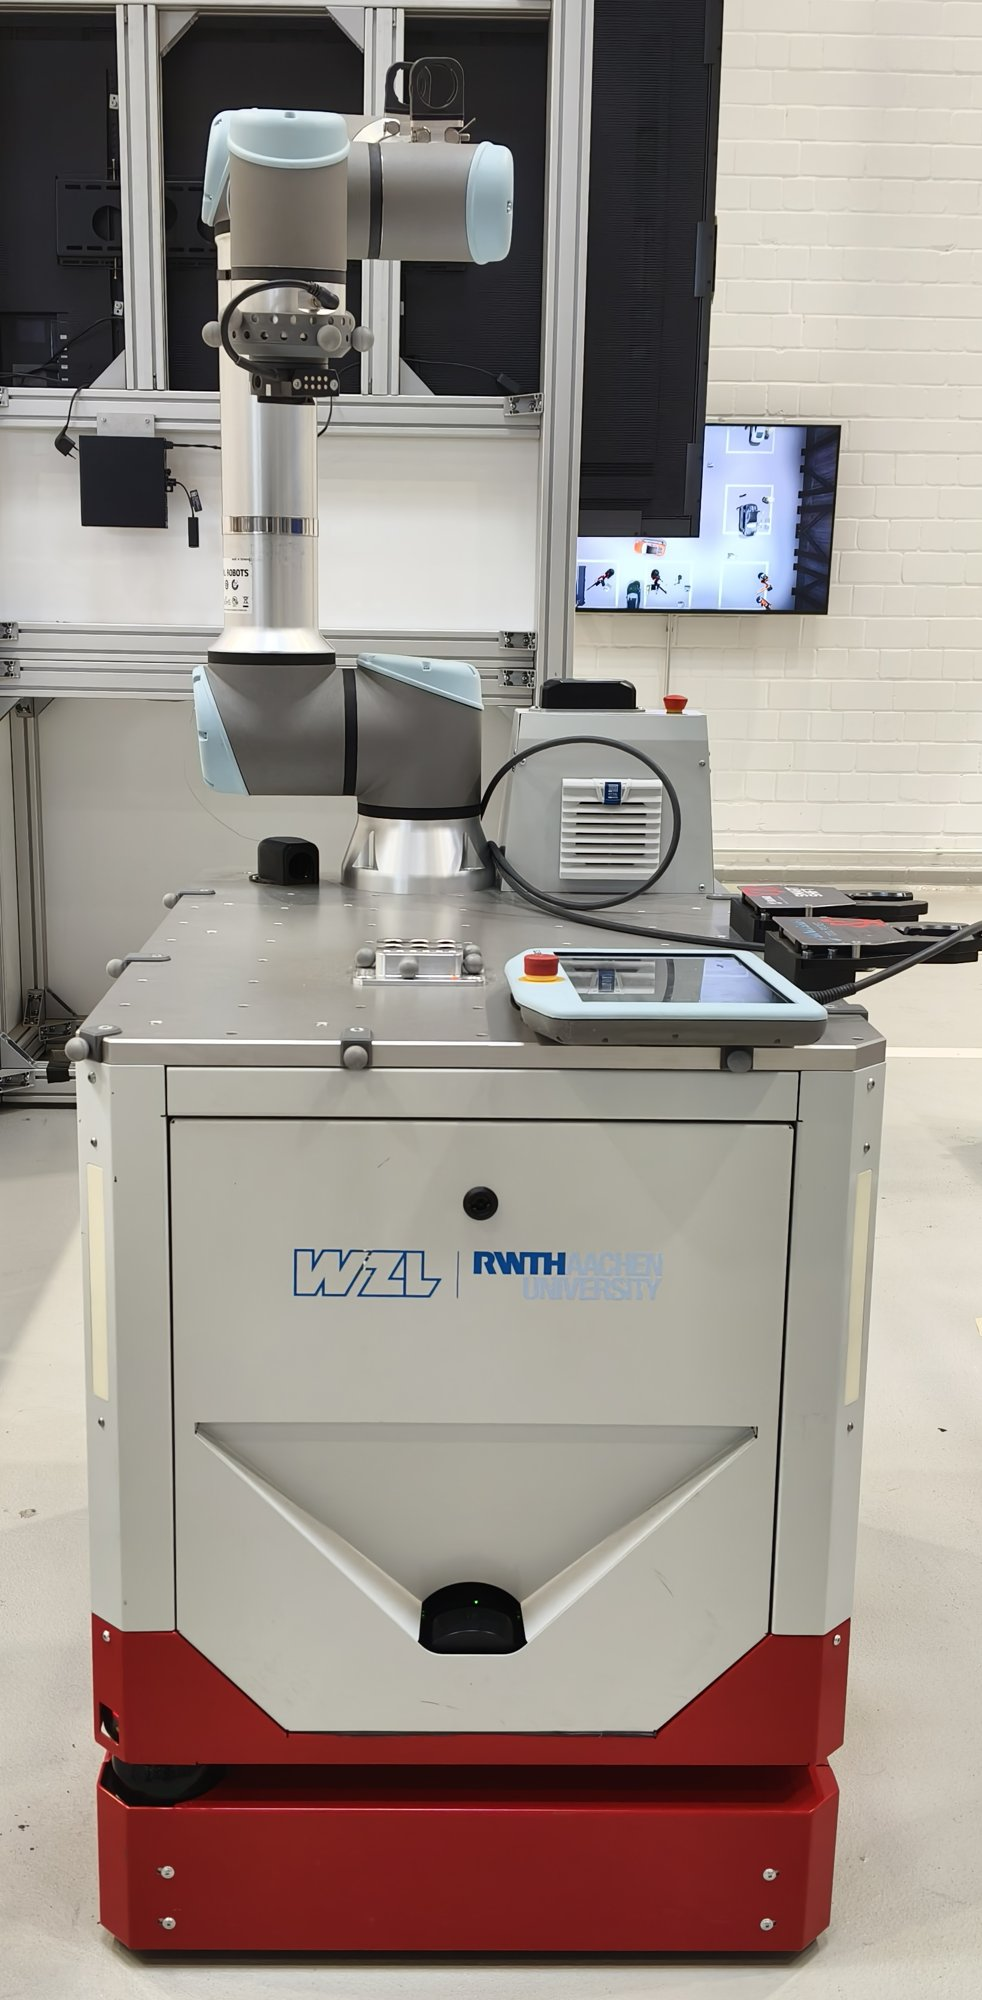
\includegraphics[width=\textwidth]{hero_view_front.jpg}
    \caption{Front}
    \label{fig:hero-photo-front}
  \end{subfigure}
  \hfill
  \begin{subfigure}[t]{0.34\textwidth}
    \centering
    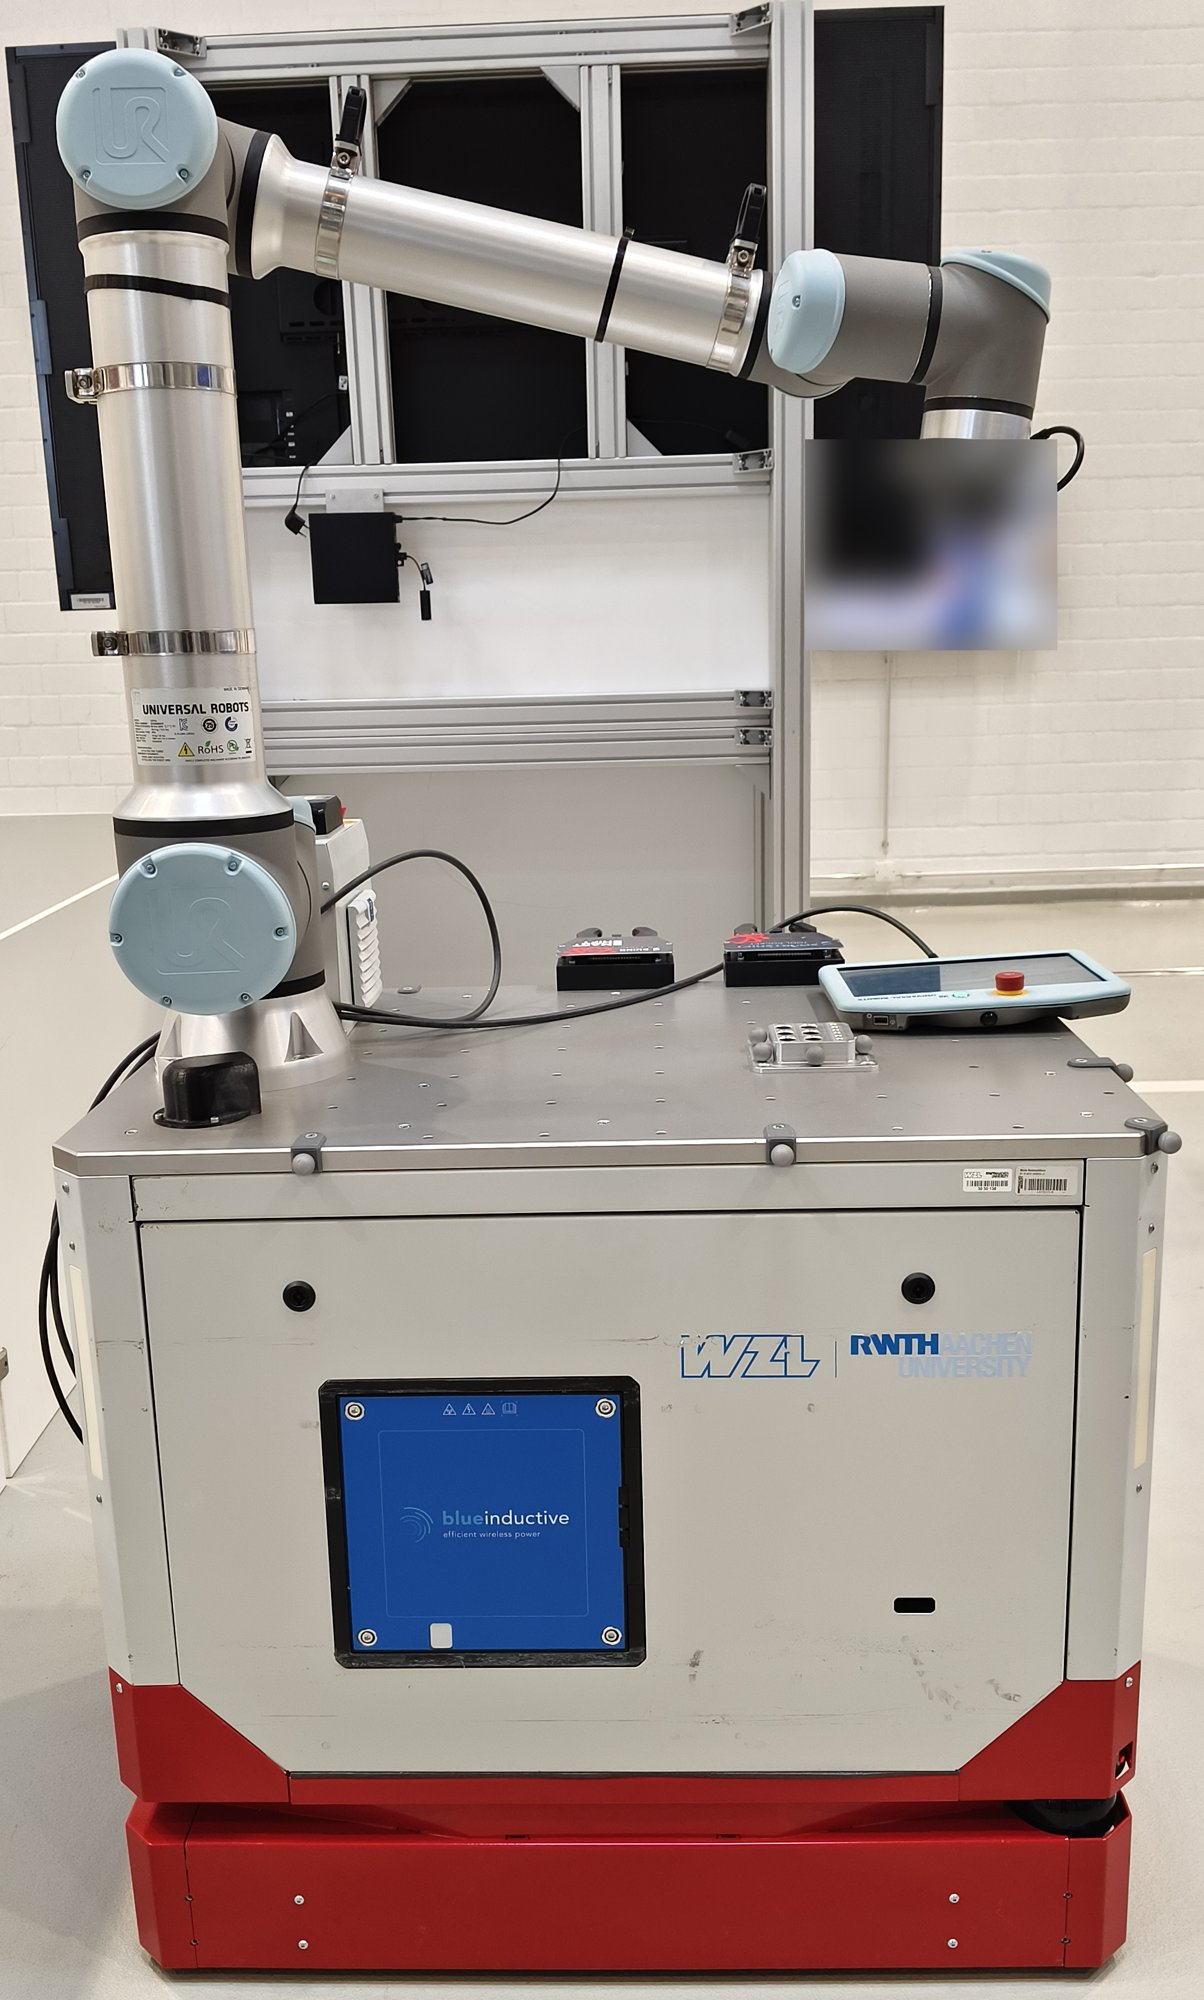
\includegraphics[width=\textwidth]{hero_view_side.jpg}
    \caption{Side}
    \label{fig:hero-photo-side}
  \end{subfigure}
  \hfill
  \begin{subfigure}[t]{0.27\textwidth}
    \centering
    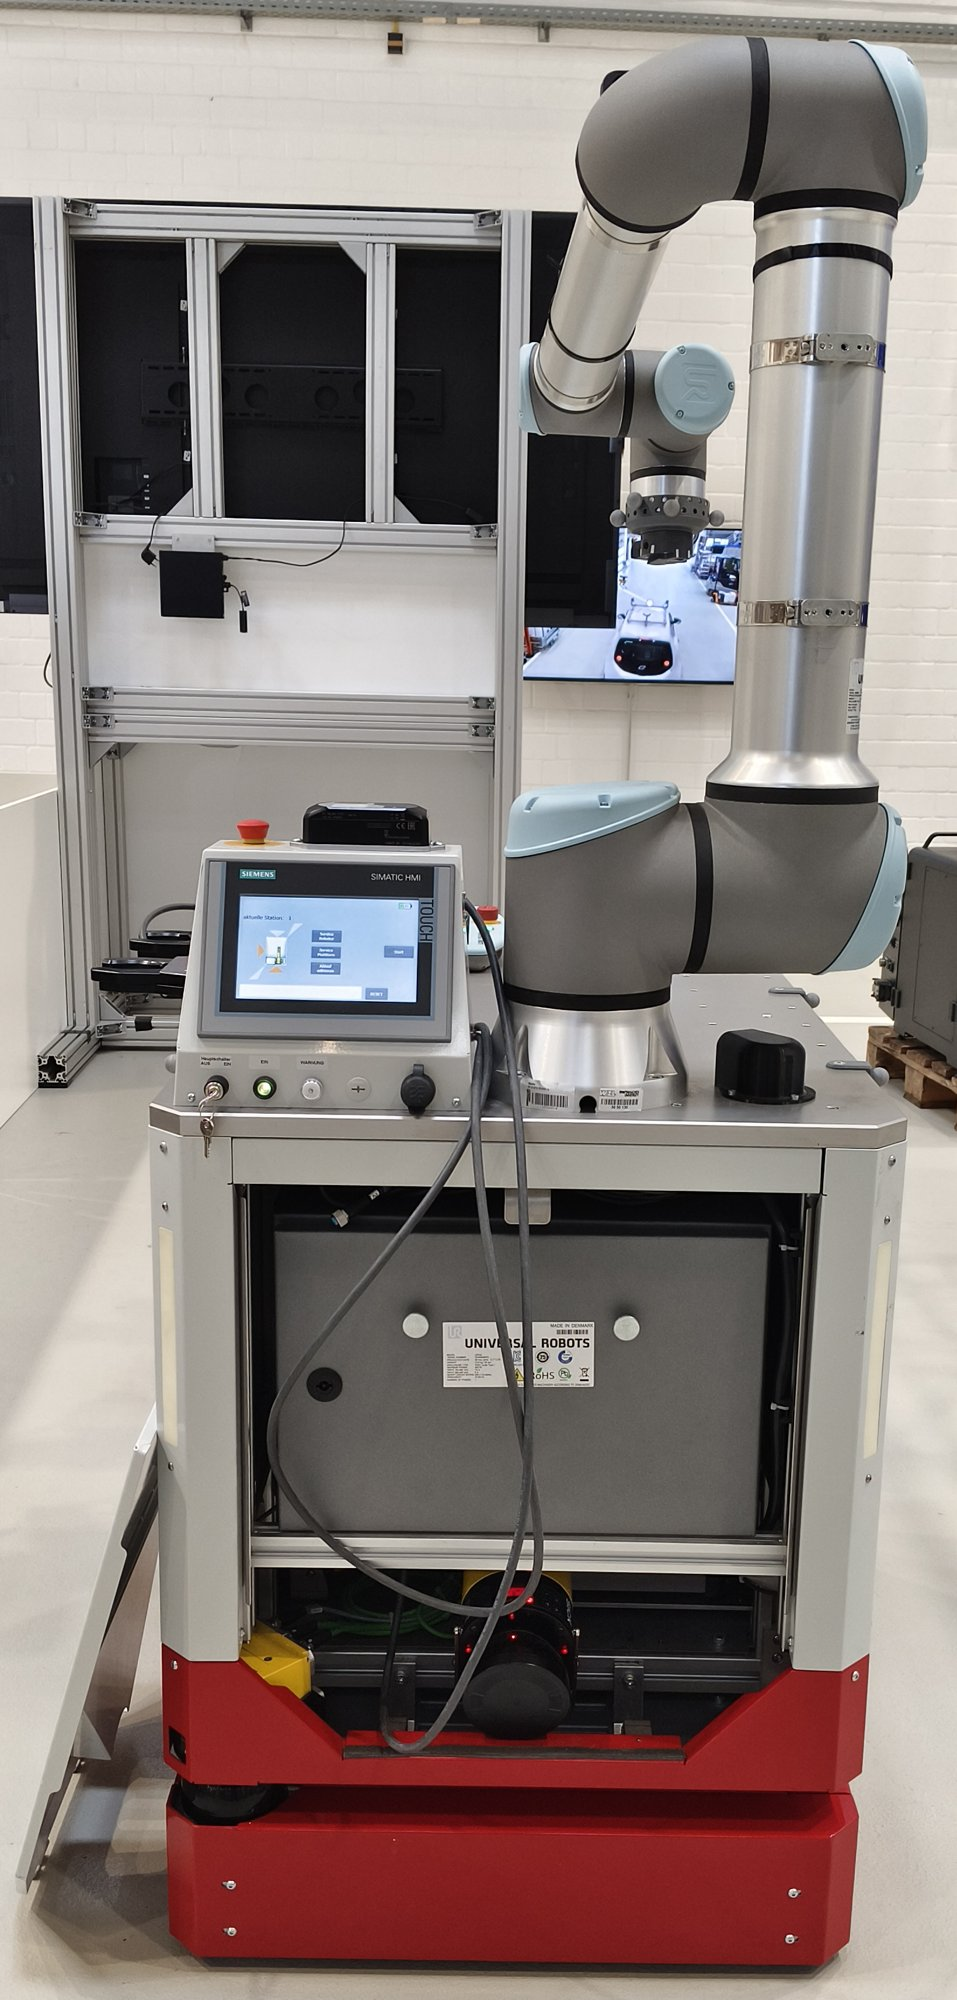
\includegraphics[width=\textwidth]{hero_view_back.jpg}
    \caption{Rear}
    \label{fig:hero-photo-rear}
  \end{subfigure}
  \caption{The \hero{} platform: UR10e arm on the \emph{freeMoVe} base
    with its red drive unit. The teach pendant lies on the top plate in
    (a) and (b). The operator panel next to the shoulder in (c) is the
    \texttt{hmi} link of the kinematic description; the UR control box
    sits inside the chassis below it.}
  \label{fig:hero-photo}
\end{figure}

Two properties of this combination shape the control problem. The first
is the drive geometry: the base pose has three planar degrees of freedom
but only two independent velocity inputs, and the base cannot translate
sideways~\cite{Lynch2017ModernRobotics}. A whole-body planner must
respect this non-holonomic restriction, otherwise it produces \ee{} paths
that the base cannot follow~\cite{Giftthaler2017Kinematic}. The second is
inertia. Moving a \qty{400}{\kilo\gram} platform is slow, and the safety
concept of the platform limits its speed independently of what a
controller may request, which is why the base velocities in
\cref{sec:wholebody-model} are capped an order of magnitude below the
arm's capability.

The kinematic tree is rooted at the frame \texttt{footprint}, which lies
on the ground plane midway between the drive wheels, with $x$ forward,
$y$ to the left and $z$ upwards. The controlled \ee{} frame is
\texttt{tool0}, the flange frame that coincides with the tool
orientation shown on the teach pendant; the arm's own
\texttt{base\_link} is not used, because its axes are rotated with
respect to the pendant convention and would invite sign errors when
comparing commanded and measured poses.

\Cref{fig:hero-frames} shows the tree, the frames it defines and the
state components attached to them.

\begin{figure}[htbp]
  \centering
  \begin{tikzpicture}[
      font=\footnotesize,
      box/.style={draw, rounded corners=1pt, align=center,
                  inner sep=3pt, minimum height=6.5mm, minimum width=23mm},
      passive/.style={box, fill=gray!12},
      ctrl/.style={box, draw=RWTHOrange100, thick},
      lbl/.style={font=\scriptsize, align=left},
      jt/.style={font=\scriptsize, align=center, inner sep=1.5pt},
      flow/.style={-{Latex[length=1.8mm]}, thick},
      note/.style={-{Latex[length=1.4mm]}, gray},
    ]
    % --- trunk ------------------------------------------------------
    \node[box]  (fp) at (0,0)     {\texttt{footprint}};
    \node[box]  (ch) at (0,-1.5)  {\texttt{chassis}};
    \node[box]  (mt) at (0,-3.4)  {\texttt{ur\_mount}};
    \node[box]  (bl) at (0,-4.7)  {\texttt{base\_link}};
    \node[box, minimum width=50mm] (ar) at (0,-6.2)
      {\texttt{shoulder\_link} $\to \cdots \to$ \texttt{wrist\_3\_link}};
    \node[ctrl] (t0) at (0,-7.7)  {\texttt{tool0}};

    % --- passive branches, all children of chassis -------------------
    \node[passive] (wh) at (4.9,-0.6) {\texttt{wheel\_left}\\\texttt{wheel\_right}};
    \node[passive] (cs) at (4.9,-2.0) {$4 \times$ caster};
    \node[passive] (hm) at (4.9,-3.1) {\texttt{hmi}};

    % --- trunk edges ------------------------------------------------
    \draw[flow] (fp) -- (ch) node[jt, midway, right=1mm] {fixed, identity};
    \draw[flow] (ch) -- (mt);
    \draw[flow] (mt) -- (bl) node[jt, midway, right=1mm] {fixed};
    \draw[flow] (bl) -- (ar) node[jt, midway, right=1mm] {6 revolute joints};
    \draw[flow] (ar) -- (t0) node[jt, midway, right=1mm] {fixed};

    % --- branch edges -----------------------------------------------
    \draw[flow] (ch.east) -- (wh.west) node[jt, pos=0.55, above, sloped] {continuous};
    \draw[flow] (ch.east) -- (cs.west);
    \draw[flow] (ch.east) -- (hm.west);

    % --- left-hand annotations --------------------------------------
    \node[lbl, anchor=east, text width=31mm] (npose) at (-2.2,0)
      {$(p_x, p_y, \psi)$: base pose\\in the inertial frame};
    \draw[note] (npose.east) -- (fp.west);

    \node[jt, anchor=east, align=right] at (-0.5,-2.45)
      {fixed,\\$(-0.355,\; -0.050,\; 0.830)\,\si{\meter}$,\\$R_z(\ang{-90})$};

    \node[lbl, anchor=east] (narm) at (-3.2,-6.2) {$\qarm \in \mathbb{R}^{6}$};
    \draw[note] (narm.east) -- (ar.west);

    % --- right-hand annotations -------------------------------------
    \node[lbl, anchor=west, text width=31mm] (nwh) at (6.3,-0.6)
      {declared \emph{fixed} in the\\Pinocchio model};
    \draw[note] (nwh.west) -- (wh.east);

    \node[lbl, anchor=west, text width=40mm] (nt0) at (2.0,-7.7)
      {controlled \ee{} frame;\\\texttt{base\_link} is not used\\as reference};
    \draw[note] (nt0.west) -- (t0.east);

    % --- footprint axes ---------------------------------------------
    \begin{scope}[shift={(-1.95,1.05)}]
      \draw[-{Latex[length=1.4mm]}] (0,0) -- (0.75,0) node[right, font=\scriptsize] {$x$};
      \draw[-{Latex[length=1.4mm]}] (0,0) -- (0,0.75) node[above, font=\scriptsize] {$z$};
      \draw[-{Latex[length=1.4mm]}] (0,0) -- (-0.45,-0.45)
        node[below left, font=\scriptsize, inner sep=1pt] {$y$};
    \end{scope}
  \end{tikzpicture}
  \caption[Kinematic tree and frame convention of \hero{}]{%
    Kinematic tree of \hero{} as the Pinocchio model sees it, with the
    transforms read from the platform description. The frame
    \texttt{footprint} lies on the ground plane midway between the drive
    wheels, at a track of \qty{0.548}{\meter} and a wheel radius of
    \qty{0.08}{\meter}. Shaded links carry no optimised degree of
    freedom: the two wheel joints are declared fixed, because the wheels
    are not part of the chain from base to \ee{}, and the casters and the
    operator panel are fixed in the description itself. The nine state
    components of \cref{eq:state-input} are attached to
    \texttt{footprint} and to the six revolute arm joints.}
  \label{fig:hero-frames}
\end{figure}

\Cref{fig:hero-frames} is a reduction. The transform tree that the
running system publishes has 51 frames and is shown in full in
\cref{fig:tf-tree}. Ten of its 50 transforms change over time: the base
pose, the six arm joints, the two wheel joints, and the pose of the
\ee{} target, which the \ocs{} visualisation adds for display. All
other frames are attachments, sensors and tool frames that are rigidly
fixed to one of the frames on the trunk.

\begin{figure}[htbp]
  \centering
  \begin{tikzpicture}[
      font=\scriptsize,
      fr/.style={draw, rounded corners=1pt, font=\scriptsize\ttfamily,
                 inner sep=2pt, minimum height=5mm, minimum width=31mm},
      side/.style={draw=gray, rounded corners=1pt, fill=gray!10,
                   font=\scriptsize\ttfamily\linespread{1}\selectfont,
                   align=left, inner sep=2.5pt, anchor=west},
      wide/.style={side, text width=76mm},
      sidemov/.style={side, draw=RWTHBlau100, fill=white},
      mov/.style={-{Latex[length=1.8mm]}, very thick, RWTHBlau100},
      fix/.style={-{Latex[length=1.6mm]}, thin},
      att/.style={gray},
      lbl/.style={font=\scriptsize\linespread{1}\selectfont, align=right},
      note/.style={-{Latex[length=1.4mm]}, gray},
    ]
    % --- trunk ------------------------------------------------------
    \node[fr] (world) at (0, 0)      {world};
    \node[fr] (fp)    at (0, -0.95)  {footprint};
    \node[fr] (ch)    at (0, -2.25)  {chassis};
    \node[fr] (mt)    at (0, -3.55)  {ur\_mount};
    \node[fr] (bl)    at (0, -4.5)   {base\_link};
    \node[fr] (bi)    at (0, -5.45)  {base\_link\_inertia};
    \node[fr] (sh)    at (0, -6.4)   {shoulder\_link};
    \node[fr] (ua)    at (0, -7.35)  {upper\_arm\_link};
    \node[fr] (fa)    at (0, -8.45)  {forearm\_link};
    \node[fr] (w1)    at (0, -9.5)   {wrist\_1\_link};
    \node[fr] (w2)    at (0, -10.4)  {wrist\_2\_link};
    \node[fr] (w3)    at (0, -11.3)  {wrist\_3\_link};
    \node[fr] (fl)    at (0, -12.2)  {flange};
    \node[fr] (t0)    at (0, -13.2)  {tool0};

    \draw[mov] (world) -- (fp);
    \draw[fix] (fp) -- (ch);
    \draw[fix] (ch) -- (mt);
    \draw[fix] (mt) -- (bl);
    \draw[fix] (bl) -- (bi);
    \draw[mov] (bi) -- (sh);
    \draw[mov] (sh) -- (ua);
    \draw[mov] (ua) -- (fa);
    \draw[mov] (fa) -- (w1);
    \draw[mov] (w1) -- (w2);
    \draw[mov] (w2) -- (w3);
    \draw[fix] (w3) -- (fl);
    \draw[fix] (fl) -- (t0);

    % --- frames that move but are not on the trunk -------------------
    \node[sidemov] (cmd) at (2.3, 0) {command};
    \draw[mov] (world.east) -- (cmd.west);
    \node[lbl, anchor=west, align=left] at (cmd.east)
      {\ee{} target, for display};
    \node[sidemov] (wh) at (2.3, -1.6) {wheel\_left, wheel\_right};
    \draw[mov] (ch.east) -- (wh.west);

    % --- frames rigidly attached to a trunk frame --------------------
    \node[wide] (chs) at (2.3, -2.95)
      {hmi\\
       caster\_front\_left, caster\_front\_right,
       caster\_rear\_left, caster\_rear\_right\\
       laser\_scanner\_front, laser\_scanner\_front\_right,
       laser\_scanner\_left, laser\_scanner\_rear,
       laser\_scanner\_rear\_left};
    \draw[att] (ch.east) -- (chs.west);
    \node[wide] (bls) at (2.3, -4.5)
      {base $\to$ \{platform\_markers, smartshift\_tool\_pocket\_A,
       smartshift\_tool\_pocket\_B\}};
    \draw[att] (bl.east) -- (bls.west);
    \node[side] (shs) at (2.3, -6.4) {ring1};
    \draw[att] (sh.east) -- (shs.west);
    \node[wide] (uas) at (2.3, -7.35)
      {ring2, ring2b, tube\_holder\_bottom\_1 $\to$ tmac\_box,
       tube\_holder\_bottom\_2};
    \draw[att] (ua.east) -- (uas.west);
    \node[wide] (fas) at (2.3, -8.45)
      {ring3, tube\_holder\_bottom\_3 $\to$ tube\_holder\_top\_3,
       tube\_holder\_bottom\_4 $\to$ tube\_holder\_top\_4};
    \draw[att] (fa.east) -- (fas.west);
    \node[side] (w1s) at (2.3, -9.5) {ring4};
    \draw[att] (w1.east) -- (w1s.west);
    \node[side] (w2s) at (2.3, -10.4) {ring5};
    \draw[att] (w2.east) -- (w2s.west);
    \node[side] (w3s) at (2.3, -11.3) {ft\_frame};
    \draw[att] (w3.east) -- (w3s.west);
    \node[wide] (t0s) at (2.3, -13.2)
      {ring6 $\to$ \{tool\_peg, tool\_tmac, smartshift\_robot\_adapter
       $\to$ smartshift\_tool\_adapter $\to$ tool\_smartshift\_mft\}};
    \draw[att] (t0.east) -- (t0s.west);

    % --- left-hand annotations --------------------------------------
    \node[lbl, anchor=west] at (0.2, -0.475)
      {base pose $(p_x, p_y, \psi)$};
    \node[lbl, anchor=east] (nfp) at (-2.3, -0.95)
      {model base frame};
    \draw[note] (nfp.east) -- (fp.west);
    \draw[RWTHBlau100, thick] (-1.85, -5.925) -- (-2.05, -5.925)
      -- (-2.05, -10.85) -- (-1.85, -10.85);
    \node[lbl, anchor=east] at (-2.2, -8.39)
      {six arm joints\\$\qarm \in \mathbb{R}^{6}$};
    \node[lbl, anchor=east] (nt0) at (-2.3, -13.2) {\ee{} frame};
    \draw[note] (nt0.east) -- (t0.west);

    % --- legend -----------------------------------------------------
    \draw[mov] (-3.9, -14.3) -- (-3.1, -14.3);
    \node[lbl, anchor=west] at (-3.0, -14.3) {changes over time};
    \draw[fix] (0.2, -14.3) -- (1.0, -14.3);
    \node[lbl, anchor=west] at (1.1, -14.3) {static};
    \node[side, minimum width=7mm, minimum height=3.2mm] at (3.0, -14.3) {};
    \node[lbl, anchor=west, align=left] at (3.8, -14.3)
      {frames fixed to the trunk frame on their left};
  \end{tikzpicture}
  \caption[Complete transform tree of \hero{}]{%
    Complete transform tree of \hero{}, redrawn from a
    \texttt{view\_frames} recording taken while the \ocs{} visualisation
    was running. The trunk runs from \texttt{world} to the \ee{} frame
    \texttt{tool0}. Thick blue arrows are the ten transforms that change
    over time; every other transform is static. A grey box lists the
    frames attached to the trunk frame on its left, and an arrow inside a
    box leads to a further child. The operator panel \texttt{hmi}, the
    tube holders and the marker rings \texttt{ring2} to \texttt{ring6}
    reappear among the bodies of the self-collision model in
    \cref{sec:wholebody-model}.}
  \label{fig:tf-tree}
\end{figure}

Beyond the drives, the platform carries five SICK safety laser scanners,
two safety controllers, wheel brakes, and an operator panel. None of
these enters the \mpc{} loop. The controller described here consumes
exactly two measurements, wheel odometry and arm joint positions, and
relies on the platform's own safety layer for protective stops. Obstacle
avoidance with respect to the environment is consequently not part of
the optimisation; only self-collision between the arm and the platform
is (\cref{sec:wholebody-model}).

Computation is split over two machines on the robot's own
\texttt{192.168.12.0/24} subnet. An industrial PC (IPC) inside the
platform hosts the ROS~2 Jazzy control stack in a container and reaches
the arm controller over the same subnet; an external PC joins
the subnet either by cable or through the platform's wireless access
point~\cite{ROS2,Macenski2022ROS2}. Which software runs where is the
subject of the next section.

% ---------------------------------------------------------------------
\section{Distributed System Architecture for Real-Time \mpc{}}
\label{sec:distributed-arch}

Solving the optimal-control problem is the most expensive part of the
loop relative to the remaining nodes on the IPC, and the IPC is the
smaller of the two machines available. It carries an Intel Core
i5-6300U with two cores and four threads and \qty{7.7}{\giga\byte} of
memory, runs a kernel without real-time patches, and keeps the CPU
frequency governor at \texttt{powersave}; the external PC carries an
AMD Ryzen~7 7840HS with eight cores and sixteen threads. The solver
alone is configured for eight threads (\cref{tab:mpc-config}), twice
what the IPC offers before the control chain takes its share, so
running it on board would have forced a shorter horizon or a coarser
model.

The MPC--MRT split of \ocs{} (\cref{sec:sota-ocs2}) removes that
constraint: the optimiser and the client that evaluates its policy are
separate processes that exchange messages, so they may live on
different machines~\cite{ocs2Toolbox}.

The deployment used here puts them on either side of the machine
boundary. The external PC runs the \mpc{} node, the target-generating
node and the visualisation, while the IPC runs the low-level control
chain and the MRT bridge. The fast path---measure, evaluate the policy,
actuate---is then entirely local to the IPC, and only three \ocs{}
streams cross the machine boundary. \Cref{tab:topology-streams} lists
what runs where and what the network carries.

\begin{table}[htbp]
  \centering
  \caption[Process placement and traffic across the machine boundary]{%
    Process placement and the traffic that crosses the external
    PC--IPC boundary. Keeping the MRT bridge on the IPC is what leaves
    the actuation path machine-local.}
  \label{tab:topology-streams}
  \begin{tabularx}{\linewidth}{@{}lX@{}}
    \toprule
    External PC
      & \mpc{} node, target node, RViz \\
    IPC
      & control chain, MRT bridge \\
    \addlinespace
    Crossing the network
      & \texttt{\_mpc\_observation} (IPC\,$\rightarrow$\,external PC,
        \qty{50}{\hz}), \texttt{\_mpc\_policy}
        (external PC\,$\rightarrow$\,IPC), \texttt{\_mpc\_reset} service
        at start-up \\
    \addlinespace
    Effect of a link outage
      & the bridge keeps evaluating the last policy locally until its
        validity window expires, then holds \\
    Clock synchronisation
      & not required \\
    \bottomrule
  \end{tabularx}
\end{table}

The last of those rows follows from where wall-clock times are compared.
\ocs{} timestamps observations and policies on a relative time axis
whose origin the bridge fixes at the first accepted measurement, so the
\mpc{}--MRT exchange itself is insensitive to an offset between the two
machine clocks. The bridge does compare wall-clock times in one place,
its staleness check on incoming measurements, and there the two operands
share the IPC clock: the bridge runs on the IPC, and odometry and joint
states are published by the control chain on the same machine. An offset
to the external PC therefore never enters the \qty{0.2}{\second}
staleness threshold, and a time service such as Chrony is not needed to
keep the loop running~\cite{Chrony}. Chrony does run on the IPC, with
the external PC as its reference; at the time of writing it reported an
offset of \qty{-0.7}{\milli\second} at an RMS of
\qty{1.5}{\milli\second}. That keeps logs recorded on the two machines
comparable, but the control loop does not depend on it.

The deployment runs with the Zenoh middleware implementation rather than
the default DDS transport of ROS~2. The switch was made during
bring-up, after DDS discovery over the platform's wireless link had
repeatedly failed to establish the \ocs{} streams; no side-by-side
comparison of the two middlewares was recorded, so this is a deployment
decision and not a measured result~\cite{zenoh,Macenski2022ROS2}.
Zenoh requires a router process on each machine, with one router
configured to connect to the other; the external PC router is pointed at
the IPC router. \Cref{fig:architecture} shows the resulting node and
topic layout.

\begin{figure}[htbp]
  \centering
  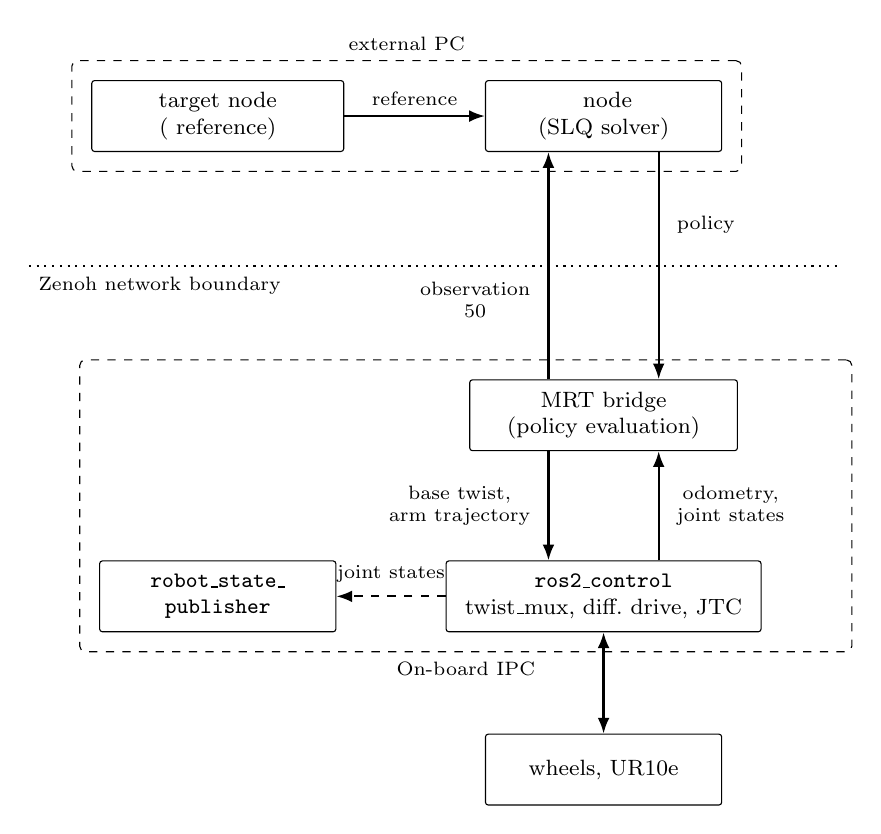
\begin{tikzpicture}[
      font=\footnotesize,
      box/.style={draw, rounded corners=1pt, align=center,
                  inner sep=4pt, minimum height=9mm},
      machine/.style={draw, dashed, rounded corners=2pt, inner sep=7pt},
      flow/.style={-{Latex[length=2mm]}, thick},
      lbl/.style={font=\scriptsize, align=center},
    ]
    % --- PC ------------------------------------------------
    \node[box, minimum width=30mm] (mpc)    at (0,0)
      {\mpc{} node\\(SLQ solver)};
    \node[box, minimum width=32mm] (target) at (-4.9,0)
      {target node\\(\ee{} reference)};
    \node[machine, fit=(mpc)(target),
          label={[lbl]above:external PC}] (host) {};

    % --- IPC --------------------------------------------------------
    \node[box, minimum width=34mm] (mrt)  at (0,-3.8)
      {MRT bridge\\(policy evaluation)};
    \node[box, minimum width=40mm] (ctrl) at (0,-6.1)
      {\texttt{ros2\_control}\\twist\_mux, diff.\ drive, JTC};
    \node[box, minimum width=30mm] (rsp)  at (-4.9,-6.1)
      {\texttt{robot\_state\_}\\\texttt{publisher}};
    \node[inner sep=0pt, minimum size=0pt] (pad) at (2.9,-4.95) {};
    \node[machine, fit=(mrt)(ctrl)(rsp)(pad),
          label={[lbl]below:On-board IPC}] (ipc) {};

    % --- robot ------------------------------------------------------
    \node[box, minimum width=30mm] (robot) at (0,-8.3)
      {wheels, UR10e};

    % --- cross-machine streams --------------------------------------
    \draw[flow] ([xshift=-7mm]mrt.north) -- ([xshift=-7mm]mpc.south)
      node[lbl, pos=0.35, left=1mm] {observation\\\qty{50}{\hz}};
    \draw[flow] ([xshift=7mm]mpc.south) -- ([xshift=7mm]mrt.north)
      node[lbl, pos=0.32, right=1mm] {policy};

    % --- local links ------------------------------------------------
    \draw[flow] (target) -- (mpc)
      node[lbl, midway, above] {reference};
    \draw[flow] ([xshift=-7mm]mrt.south) -- ([xshift=-7mm]ctrl.north)
      node[lbl, midway, left=1mm] {base twist,\\arm trajectory};
    \draw[flow] ([xshift=7mm]ctrl.north) -- ([xshift=7mm]mrt.south)
      node[lbl, midway, right=1mm] {odometry,\\joint states};
    \draw[flow, {Latex[length=2mm]}-{Latex[length=2mm]}]
      (ctrl.south) -- (robot.north);
    \draw[flow, dashed] (ctrl.west) -- (rsp.east)
      node[lbl, midway, above=0.5mm] {joint states};

    % --- network boundary -------------------------------------------
    \draw[dotted, thick] (-7.3,-1.9) -- (3.0,-1.9);
    \node[lbl, anchor=west] at (-7.3,-2.15) {Zenoh network boundary};
  \end{tikzpicture}
  \caption[Deployment of \ocs{} on \hero{}]{%
    Deployment of \ocs{} on \hero{}. The external PC solves the
    optimal-control problem; the IPC evaluates the resulting policy and
    actuates the robot, so the loop that runs at \qty{50}{\hz} is
    machine-local. The reset service and the visualisation on the
    external PC are omitted.}
  \label{fig:architecture}
\end{figure}

One consistency requirement is easy to violate and is stated here
explicitly. The \mpc{} node and the MRT bridge each build their own
Pinocchio model from a URDF file that is exported from the platform
description at launch time~\cite{Carpentier2019Pinocchio}. The two
exports must use the same end-effector variant and the same kinematic
calibration file, otherwise the solver optimises for one robot and the
bridge evaluates the policy on another. The visualisation, in contrast, takes its model from the
\texttt{robot\_state\_publisher} on the IPC, which is the single
authoritative source of \texttt{/tf} and \texttt{/robot\_description};
the external PC launch deliberately starts no second publisher. Because
\ocs{} hardcodes \texttt{world} as its inertial frame while the robot
tree is rooted at \texttt{odom}, an identity transform between the two
is published on the external PC. The base state fed to the solver is
wheel odometry, so \texttt{world} and \texttt{odom} coincide
numerically; the price is that the controller inherits the drift of the
odometry, and no external localisation corrects it.

Start-up follows a fixed order: the Zenoh routers first, then the
\mpc{} node on the external PC, then the IPC. The \mpc{} node advertises
the reset service that the bridge needs for its initial handshake, so
starting it first avoids a wait. The reverse order also converges,
because the bridge waits for the service rather than aborting
(\cref{sec:hw-interfaces}). On the first start after a model change,
\ocs{} generates and compiles the derivative code before the solver
runs, which adds a delay of roughly one minute; the compiled libraries
are then cached on disk.

% ---------------------------------------------------------------------
\section{Whole-Body Model and Parameterisation}
\label{sec:wholebody-model}

\ocs{} ships a mobile-manipulator model family, of which the
\emph{wheel-based} variant matches \hero{}: a non-holonomic planar base
carrying a serial arm~\cite{ocs2Toolbox}. The Pinocchio model is built
from the platform URDF with the two wheel joints declared fixed, since
the wheels are not part of the kinematic chain from base to \ee{} and
their rotation is irrelevant to the
task~\cite{Carpentier2019Pinocchio}. The base frame is \texttt{footprint}
and the \ee{} frame is \texttt{tool0}, as introduced in
\cref{sec:hero-platform}. The resulting state and input are

\begin{equation}
  \svec = \left( p_x,\; p_y,\; \psi,\; \qarm \right) \in \mathbb{R}^{9},
  \qquad
  \uvec = \left( v,\; \omega,\; \qarmdot \right) \in \mathbb{R}^{8},
  \label{eq:state-input}
\end{equation}

with $(p_x, p_y, \psi)$ the base pose in the inertial frame,
$\qarm \in \mathbb{R}^{6}$ the arm joint positions, $v$ and $\omega$ the
base forward and yaw rate, and $\qarmdot$ the arm joint velocities.
The system equation is the differential-drive kinematics augmented by
the arm joints~\cite{Lynch2017ModernRobotics},

\begin{equation}
  \dot{\svec} \;=\; f(\svec, \uvec) \;=\;
  \begin{pmatrix}
    v \cos\psi \\ v \sin\psi \\ \omega \\ \qarmdot
  \end{pmatrix} ,
  \label{eq:flowmap}
\end{equation}

which encodes the non-holonomic restriction of
\cref{sec:hero-platform}: no input produces motion along the base
$y$-axis. The model is kinematic, not dynamic. The control chain used
here issues only a twist to the drive controller and position setpoints,
at a fixed rate, to the joint-trajectory controller. No validated
inertial parameters exist for the loaded platform either. A dynamic
model would therefore add eight velocity states ($v$, $\omega$ and the
six arm joint rates) and an unverified mass matrix, while the commands
that reach the actuators would remain twists and joint positions. The
cost of this choice is that inertial effects appear to the solver only
through the velocity limits.

The objective combines an input cost with soft constraints. Over a
horizon $T$ starting at $t_0$,

\begin{equation}
  \begin{aligned}
    J = \int_{t_0}^{t_0+T} \Big[
        &\tfrac{1}{2}\, \uvec^{\mathsf{T}} R\, \uvec
      + \tfrac{1}{2}\, \mu_\mathrm{p} \lVert e_\mathrm{p}(\svec) \rVert^2
      + \tfrac{1}{2}\, \mu_\mathrm{o} \lVert e_\mathrm{o}(\svec) \rVert^2 \\
      &+ B_\mathrm{lim}(\svec, \uvec) + B_\mathrm{col}(\svec)
      \Big]\, \mathrm{d}t
      \;+\; \Phi\big(\svec(t_0+T)\big) ,
  \end{aligned}
  \label{eq:cost}
\end{equation}

where $e_\mathrm{p}$ is the \ee{} position error and $e_\mathrm{o}$ the
orientation error, both taken with respect to the reference pose
interpolated from the target trajectory at the current time, and $\Phi$
repeats the two \ee{} terms at the end of the horizon. The reference is
supplied online through the \ocs{} reference manager, either by an
interactive marker in RViz or by the waypoint node used in
\cref{ch:simulation,ch:hardware}. \ocs{} interpolates that reference
linearly and component-wise between successive knots, the quaternion
included, which is why the waypoint node commands one constant
orientation for the whole path (\cref{sec:sim-path}).
\Cref{fig:cost-structure} collects the terms and the quantities each of
them acts on.

\begin{figure}[htbp]
  \centering
  \begin{tikzpicture}[
      font=\footnotesize,
      term/.style={draw, rounded corners=1pt, align=center, inner sep=3.5pt,
                   minimum height=7.5mm, minimum width=30mm},
      tgt/.style={draw, rounded corners=1pt, align=center, inner sep=3.5pt,
                  minimum height=7.5mm, minimum width=36mm, fill=gray!10},
      ref/.style={draw, rounded corners=1pt, align=center, inner sep=3pt,
                  minimum height=6.5mm, minimum width=36mm,
                  draw=RWTHBlau100},
      flow/.style={-{Latex[length=1.8mm]}, thick},
      wk/.style={font=\scriptsize, align=left},
      lbl/.style={font=\scriptsize, align=center},
    ]
    % --- cost terms ---------------------------------------------------
    \node[term] (r)   at (0,0)    {$\tfrac{1}{2}\,\uvec^{\mathsf{T}} R\, \uvec$};
    \node[term] (ep)  at (0,-1.15) {$\tfrac{1}{2}\, \mu_\mathrm{p} \lVert e_\mathrm{p} \rVert^2$};
    \node[term] (eo)  at (0,-2.30) {$\tfrac{1}{2}\, \mu_\mathrm{o} \lVert e_\mathrm{o} \rVert^2$};
    \node[term] (bl)  at (0,-3.45) {$B_\mathrm{lim}(\svec, \uvec)$};
    \node[term] (bc)  at (0,-4.60) {$B_\mathrm{col}(\svec)$};
    \node[term] (phi) at (0,-5.75) {$\Phi\big(\svec(t_0+T)\big)$};

    % --- configured values --------------------------------------------
    \node[wk, anchor=east] at (-1.75,0)     {$R_\mathrm{base} = 0.085\, I_2$,\\$R_\mathrm{arm} = 0.04\, I_6$};
    \node[wk, anchor=east] at (-1.75,-1.15) {$\mu_\mathrm{p} = 10$};
    \node[wk, anchor=east] at (-1.75,-2.30) {$\mu_\mathrm{o} = 5$};
    \node[wk, anchor=east] at (-1.75,-3.45) {panel joint limits,\\velocity bounds on all\\eight inputs};
    \node[wk, anchor=east] at (-1.75,-4.60) {12 link pairs,\\margin \qty{0.11}{\meter}};
    \node[wk, anchor=east] at (-1.75,-5.75) {repeats $\mu_\mathrm{p}$, $\mu_\mathrm{o}$\\at the horizon end};

    % --- targets --------------------------------------------------------
    \node[tgt] (u) at (5.2,0)     {input $\uvec = (v, \omega, \qarmdot)$};
    \node[tgt] (e) at (5.2,-1.95) {\ee{} pose error against\\the reference pose};
    \node[tgt] (x) at (5.2,-4.30) {state $\svec$};

    % --- reference chain -------------------------------------------------
    \node[ref] (src) at (5.2,-6.5)
      {interactive marker or\\waypoint node};
    \node[ref] (int) at (5.2,-8.0)
      {component-wise linear\\interpolation, quaternion\\included};
    \draw[flow, RWTHBlau100] (src) -- (int);
    \draw[flow, RWTHBlau100] (int.east) -- ++(1.1,0) |- (e.east);

    % --- term to target ---------------------------------------------------
    \draw[flow] (r)   -- (u);
    \draw[flow] (ep.east)  -- (e.west);
    \draw[flow] (eo.east)  -- (e.west);
    \draw[flow] (bl.east)  -- (x.west);
    \draw[flow] (bl.east)  -- (u.west);
    \draw[flow] (bc.east)  -- (x.west);
    \draw[flow, dashed] (phi.east) -- (2.75,-5.75) |- ([yshift=-2.5mm]e.west);
  \end{tikzpicture}
  \caption[Structure of the \ocs{} objective on \hero{}]{%
    Terms of the objective in \cref{eq:cost}, the values configured for
    them in \cref{tab:mpc-config}, and the quantities each term acts on.
    The ratio between $R_\mathrm{base}$ and $R_\mathrm{arm}$ is what
    distributes a commanded \ee{} motion between base and arm. In blue,
    the path by which the reference reaches the two \ee{} terms: the
    reference manager interpolates between successive knots
    component-wise, the quaternion included, which is why the waypoint
    node commands one constant orientation for a whole path.}
  \label{fig:cost-structure}
\end{figure}

The input weight is diagonal and separates base from arm,
$R = \operatorname{diag}(R_\mathrm{base}, R_\mathrm{arm})$ with
$R_\mathrm{base} = 0.085 \cdot I_2$ and
$R_\mathrm{arm} = 0.04 \cdot I_6$. The ratio is the tuning knob that
distributes a commanded \ee{} motion between base and arm: base motion
is charged roughly twice as much as arm motion, which keeps the heavy
platform still for targets the arm can reach on its own and lets it
contribute once the arm approaches its reach limit. \Cref{ch:hardware}
returns to this ratio, because it also determines whether the base
starts moving early enough for paths that leave the arm's workspace.

Limits and self-collision enter as relaxed barrier penalties, the
\ocs{} treatment of an inequality
$h(\svec,\uvec) \ge 0$~\cite{Feller2017RelaxedBarrier,ocs2Toolbox}:

\begin{equation}
  B(h) =
  \begin{cases}
    -\mu \ln h, & h > \delta, \\[2pt]
    -\mu \ln \delta
      + \dfrac{\mu}{2}\left[ \left(\dfrac{h - 2\delta}{\delta}\right)^{2} - 1 \right],
      & h \le \delta .
  \end{cases}
  \label{eq:barrier}
\end{equation}

The barrier is logarithmic while the constraint is comfortably
satisfied and switches to a quadratic extension below the relaxation
width $\delta$, which keeps the cost and its derivatives finite when a
constraint is violated---necessary here, because measured states from
the real robot do occasionally violate a limit. \Cref{fig:barrier}
shows the penalty at the configured relaxation width.

\begin{figure}[htbp]
  \centering
  \begin{tikzpicture}
    \begin{axis}[
        width=0.88\linewidth, height=5.2cm,
        xlabel={constraint slack $h$ / \si{\milli\meter}},
        ylabel={$B(h)$},
        xmin=-3, xmax=20, ymin=0, ymax=0.2,
        scaled y ticks=false,
        yticklabel style={/pgf/number format/fixed,
                          /pgf/number format/precision=2},
        legend pos=north east,
      ]
      \addplot[RWTHOrange100, thick, domain=-3:1, samples=90]
        {-0.01*ln(0.001) + 0.005*((x-2)^2 - 1)};
      \addplot[RWTHBlau100, thick, domain=1:20, samples=200]
        {-0.01*ln(x/1000)};
      \addplot[black, dashed, forget plot] coordinates {(1,0) (1,0.2)};
      \legend{quadratic extension, $-\mu \ln h$}
      \node[anchor=south west, font=\scriptsize] at (axis cs:1.3,0.155)
        {$\delta = \qty{1}{\milli\meter}$};
    \end{axis}
  \end{tikzpicture}
  \caption[Relaxed barrier penalty at the configured relaxation width]{%
    Relaxed barrier penalty of \cref{eq:barrier} at the values configured
    for the self-collision term, $\mu = \num{e-2}$ and
    $\delta = \qty{1}{\milli\meter}$. The slack $h$ is the amount by
    which a constraint is satisfied, so $h = 0$ is the constraint
    boundary and $h < 0$ a violation. Left of $\delta$ the logarithm is
    replaced by its quadratic extension, which keeps the penalty and its
    derivatives finite for the violated states that the real robot
    occasionally reports. For self-collision the slack is the distance of
    a link pair minus the \qty{0.11}{\meter} margin, so the quadratic
    extension acts only on a pair that is closer than
    $\qty{0.11}{\meter} + \delta$.}
  \label{fig:barrier}
\end{figure}

Three groups of
constraints use this penalty: arm joint position limits, velocity limits
on all eight inputs, and a minimum distance between selected pairs of
links. The position limits are overridden in the task file instead of
being read from the URDF, which bounds every UR10e joint at
\ang{\pm 360}. Those bounds are far wider than the joint limits
configured in the arm's own safety panel, so a plan that satisfies the
URDF can still drive the arm into a safety limit and provoke a
protective stop that \ocs{} never sees. The task file therefore copies
the Normal-mode panel limits of the installation used in this work
(\cref{fig:pendant-limits}): \ang{-183} to \ang{3} for the base and
shoulder joints, \ang{\pm 153} for the elbow, \ang{-228} to \ang{48}
for wrist~1, \ang{\pm 138} for wrist~2 and \ang{\pm 183} for wrist~3.
The velocity bounds are \qty{\pm 0.1}{\meter\per\second} and
\qty{\pm 0.1}{\radian\per\second} for the base and
\qty{\pm 0.3}{\radian\per\second} per arm joint, matching the caps that
the bridge enforces downstream (\cref{sec:hw-interfaces}).

\begin{figure}[htbp]
  \centering
  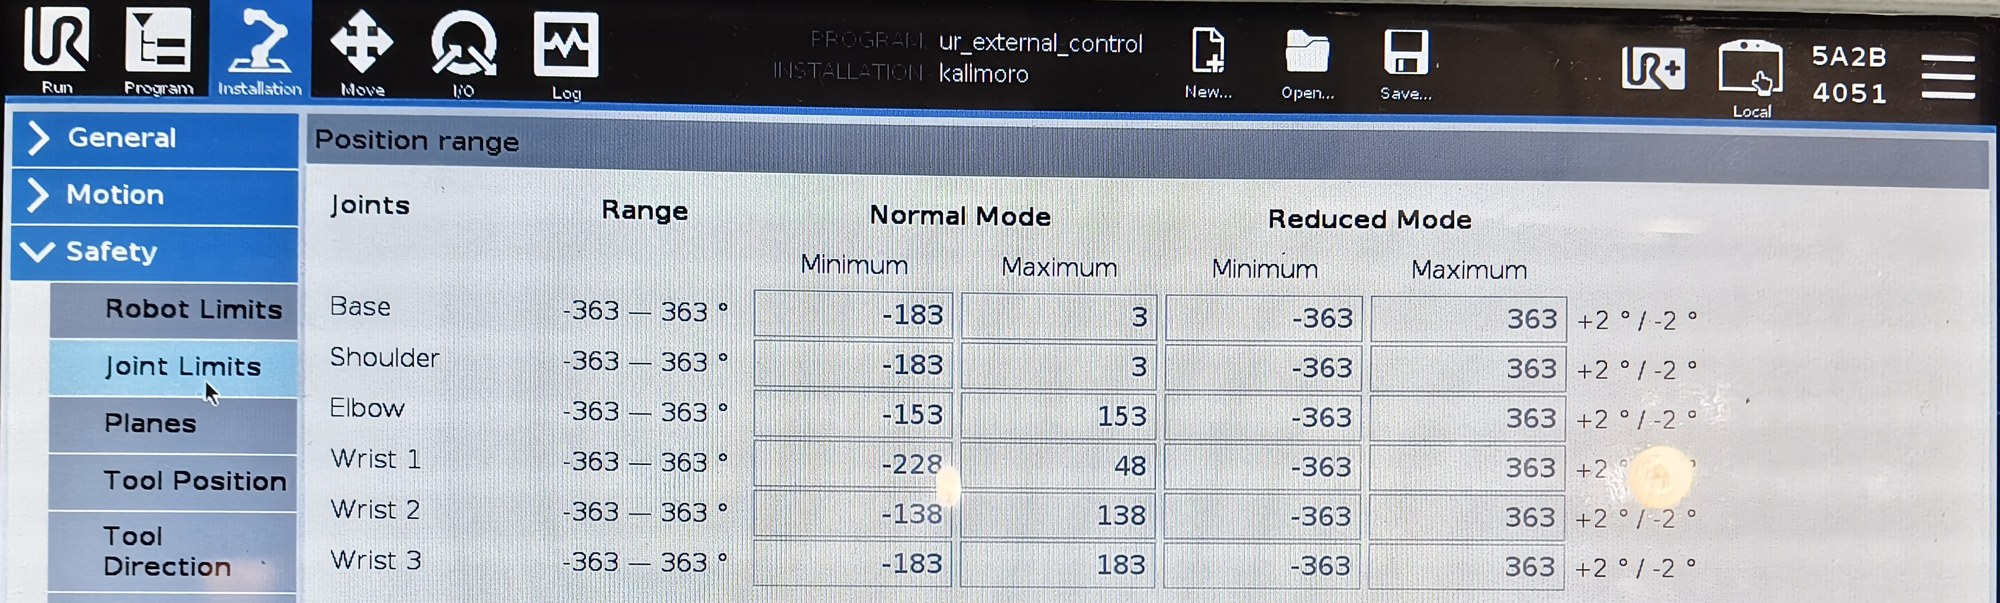
\includegraphics[width=\textwidth]{ur_pendant_joint_limits.jpg}
  \caption{Joint-limit page of the UR10e safety configuration on the
    teach pendant, installation \texttt{kalimoro}. The Normal-mode
    ranges equal the bounds in \texttt{task\_hardware.info}; the
    Reduced-mode ranges are not used in this work.}
  \label{fig:pendant-limits}
\end{figure}

Self-collision is singled out here because its evaluation cost scales
with the number of geometry pairs, and it was therefore the first term
addressed when solve time had to be reduced. Every pair costs a distance
query and its derivative with respect to the state at each node of the
time grid on which the solver linearises the
problem~\cite{Carpentier2019Pinocchio}. That grid comes from the
rollout and not from the \qty{2}{\milli\second} step at which the
backward pass integrates the Riccati equation; since the rollout
integrates adaptively, the number of nodes follows the solution rather
than the horizon~\cite{ocs2Toolbox}. It can be counted from the
recordings, because a published policy carries the solver's own grid
without resampling: over the 713 policies of the hardware lap of
\cref{ch:hardware}, one solve spans a median of ten nodes across the
\qty{1.24}{\second} it publishes, with a quartile range of nine to ten,
and the first interval equals the requested
\qty{10}{\milli\second} rollout step of \cref{tab:mpc-config} in every
one of them. Cutting the pair set from 32 to 12 therefore removes about
two hundred distance queries, and as many derivative evaluations, from
each solve. The constraint value of a pair is its distance minus the
minimum distance~\cite{ocs2Toolbox}.

Two platform bodies are within reach of the arm. The chassis top is the
mounting plane of the arm, and the shoulder axis lies only about
\qty{0.18}{\meter} above it; the operator panel (\texttt{hmi}), a box of
\qty{0.21}{\meter} $\times$ \qty{0.30}{\meter} $\times$
\qty{0.25}{\meter}, starts \qty{0.075}{\meter} beside the shoulder axis
and covers the height of the shoulder. On the arm side, the five moving
links from \texttt{upper\_arm\_link} to \texttt{wrist\_3\_link} carry
attachments: six marker rings of the motion capture system, which
protrude at most about \qty{1}{\centi\meter} from the link surface, and
six tube holders, which protrude about
\qtyrange{3}{6}{\centi\meter} (\cref{fig:collision-photos}). Pairing both platform bodies with these links and
attachments gave the original set of 32 pairs. Pairs whose distance does
not change with the arm configuration, such as the shoulder link against
the chassis, were never part of it.

\begin{figure}[htbp]
  \centering
  \begin{subfigure}[t]{0.40\textwidth}
    \centering
    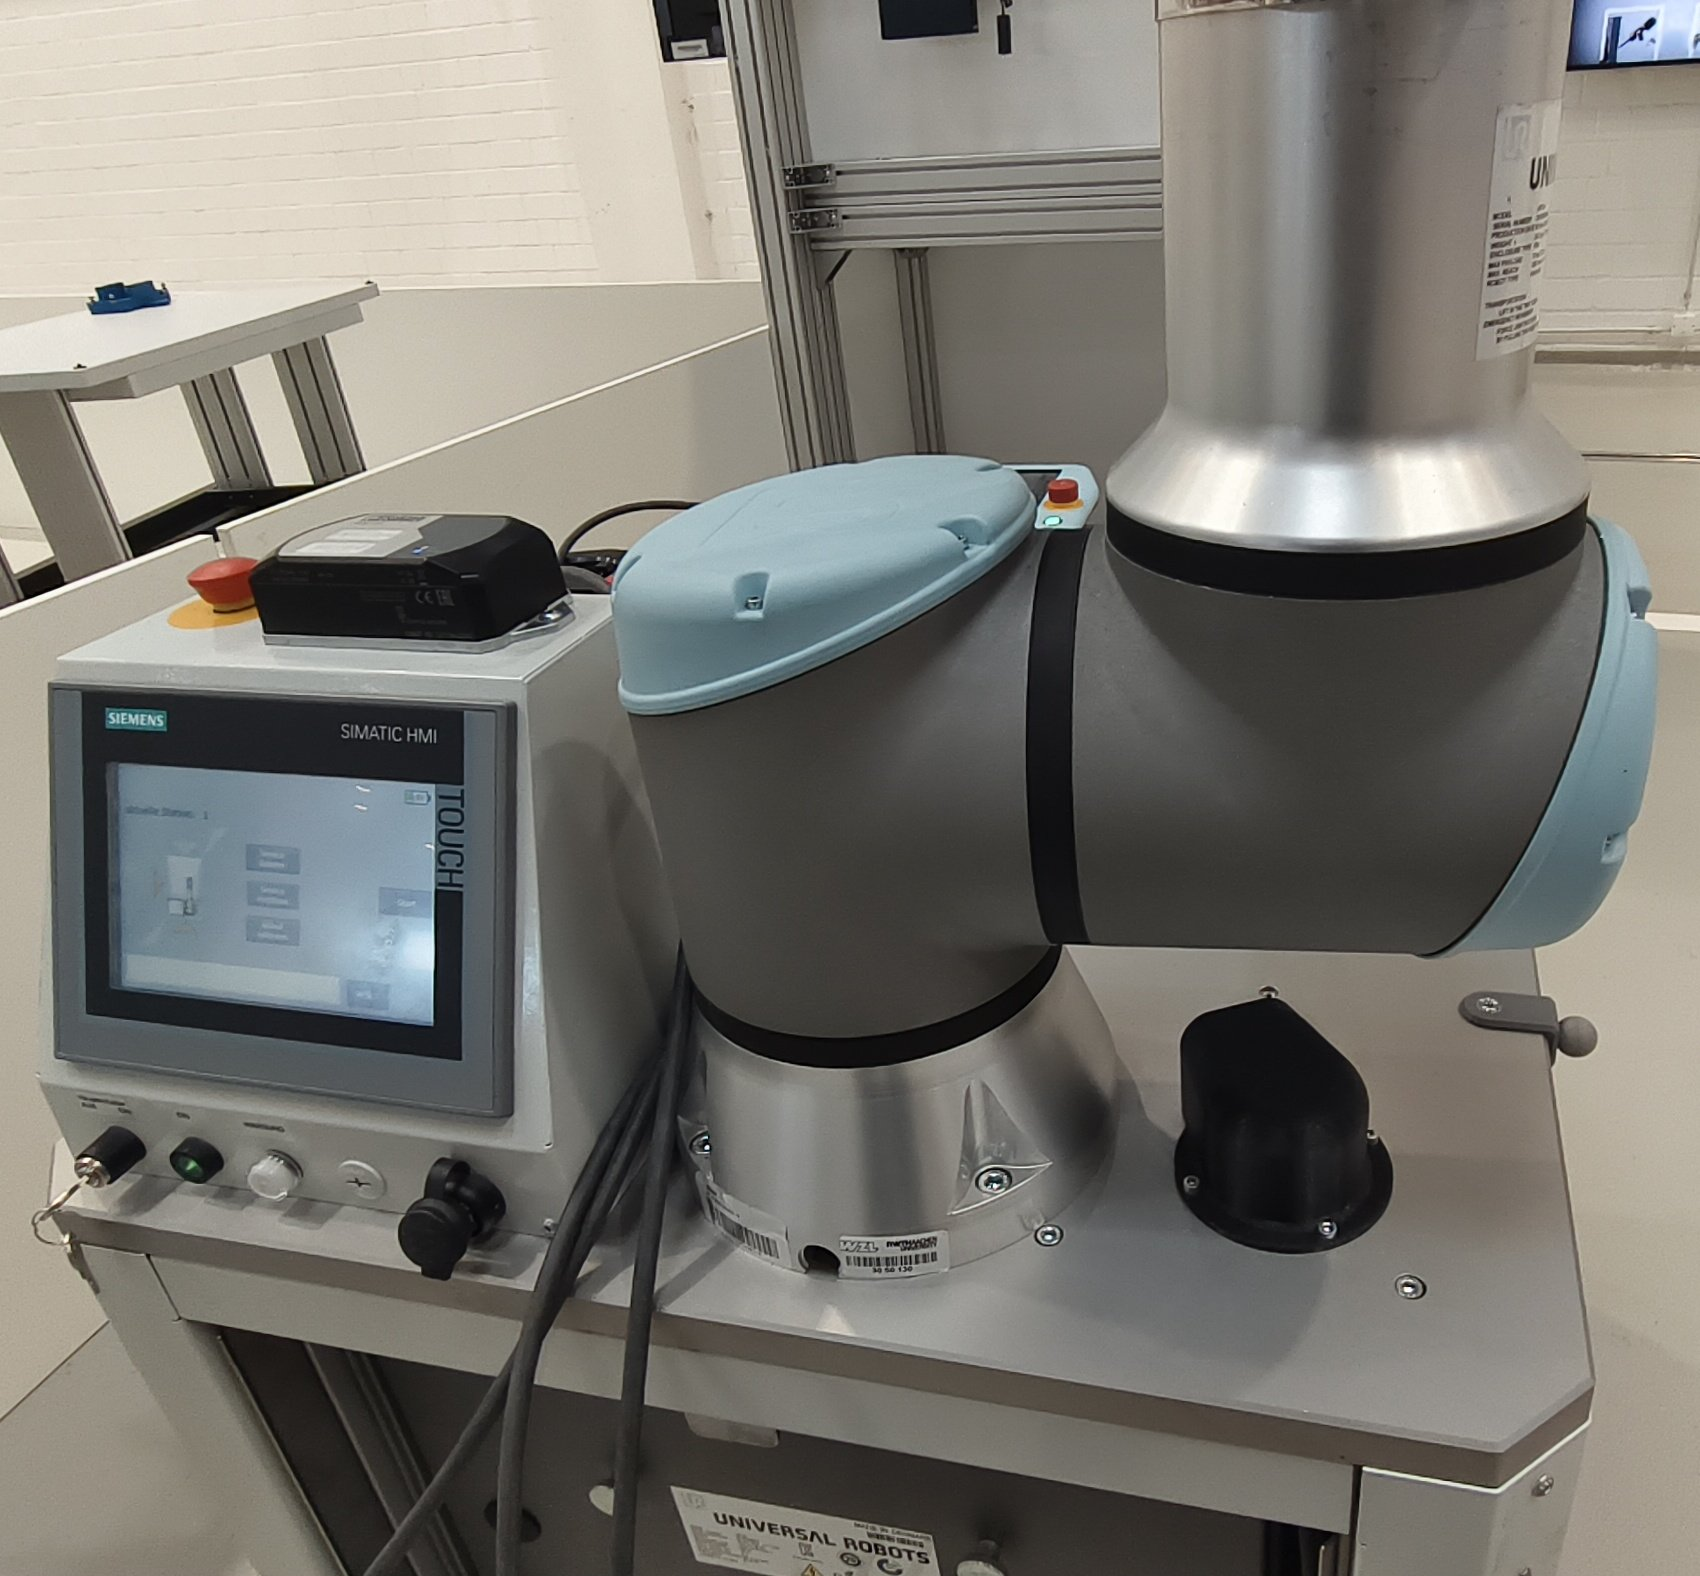
\includegraphics[height=5cm]{hero_arm_mount.jpg}
    \caption{Arm base on the chassis top, next to the operator panel
      (\texttt{hmi}).}
    \label{fig:collision-photo-mount}
  \end{subfigure}
  \hfill
  \begin{subfigure}[t]{0.27\textwidth}
    \centering
    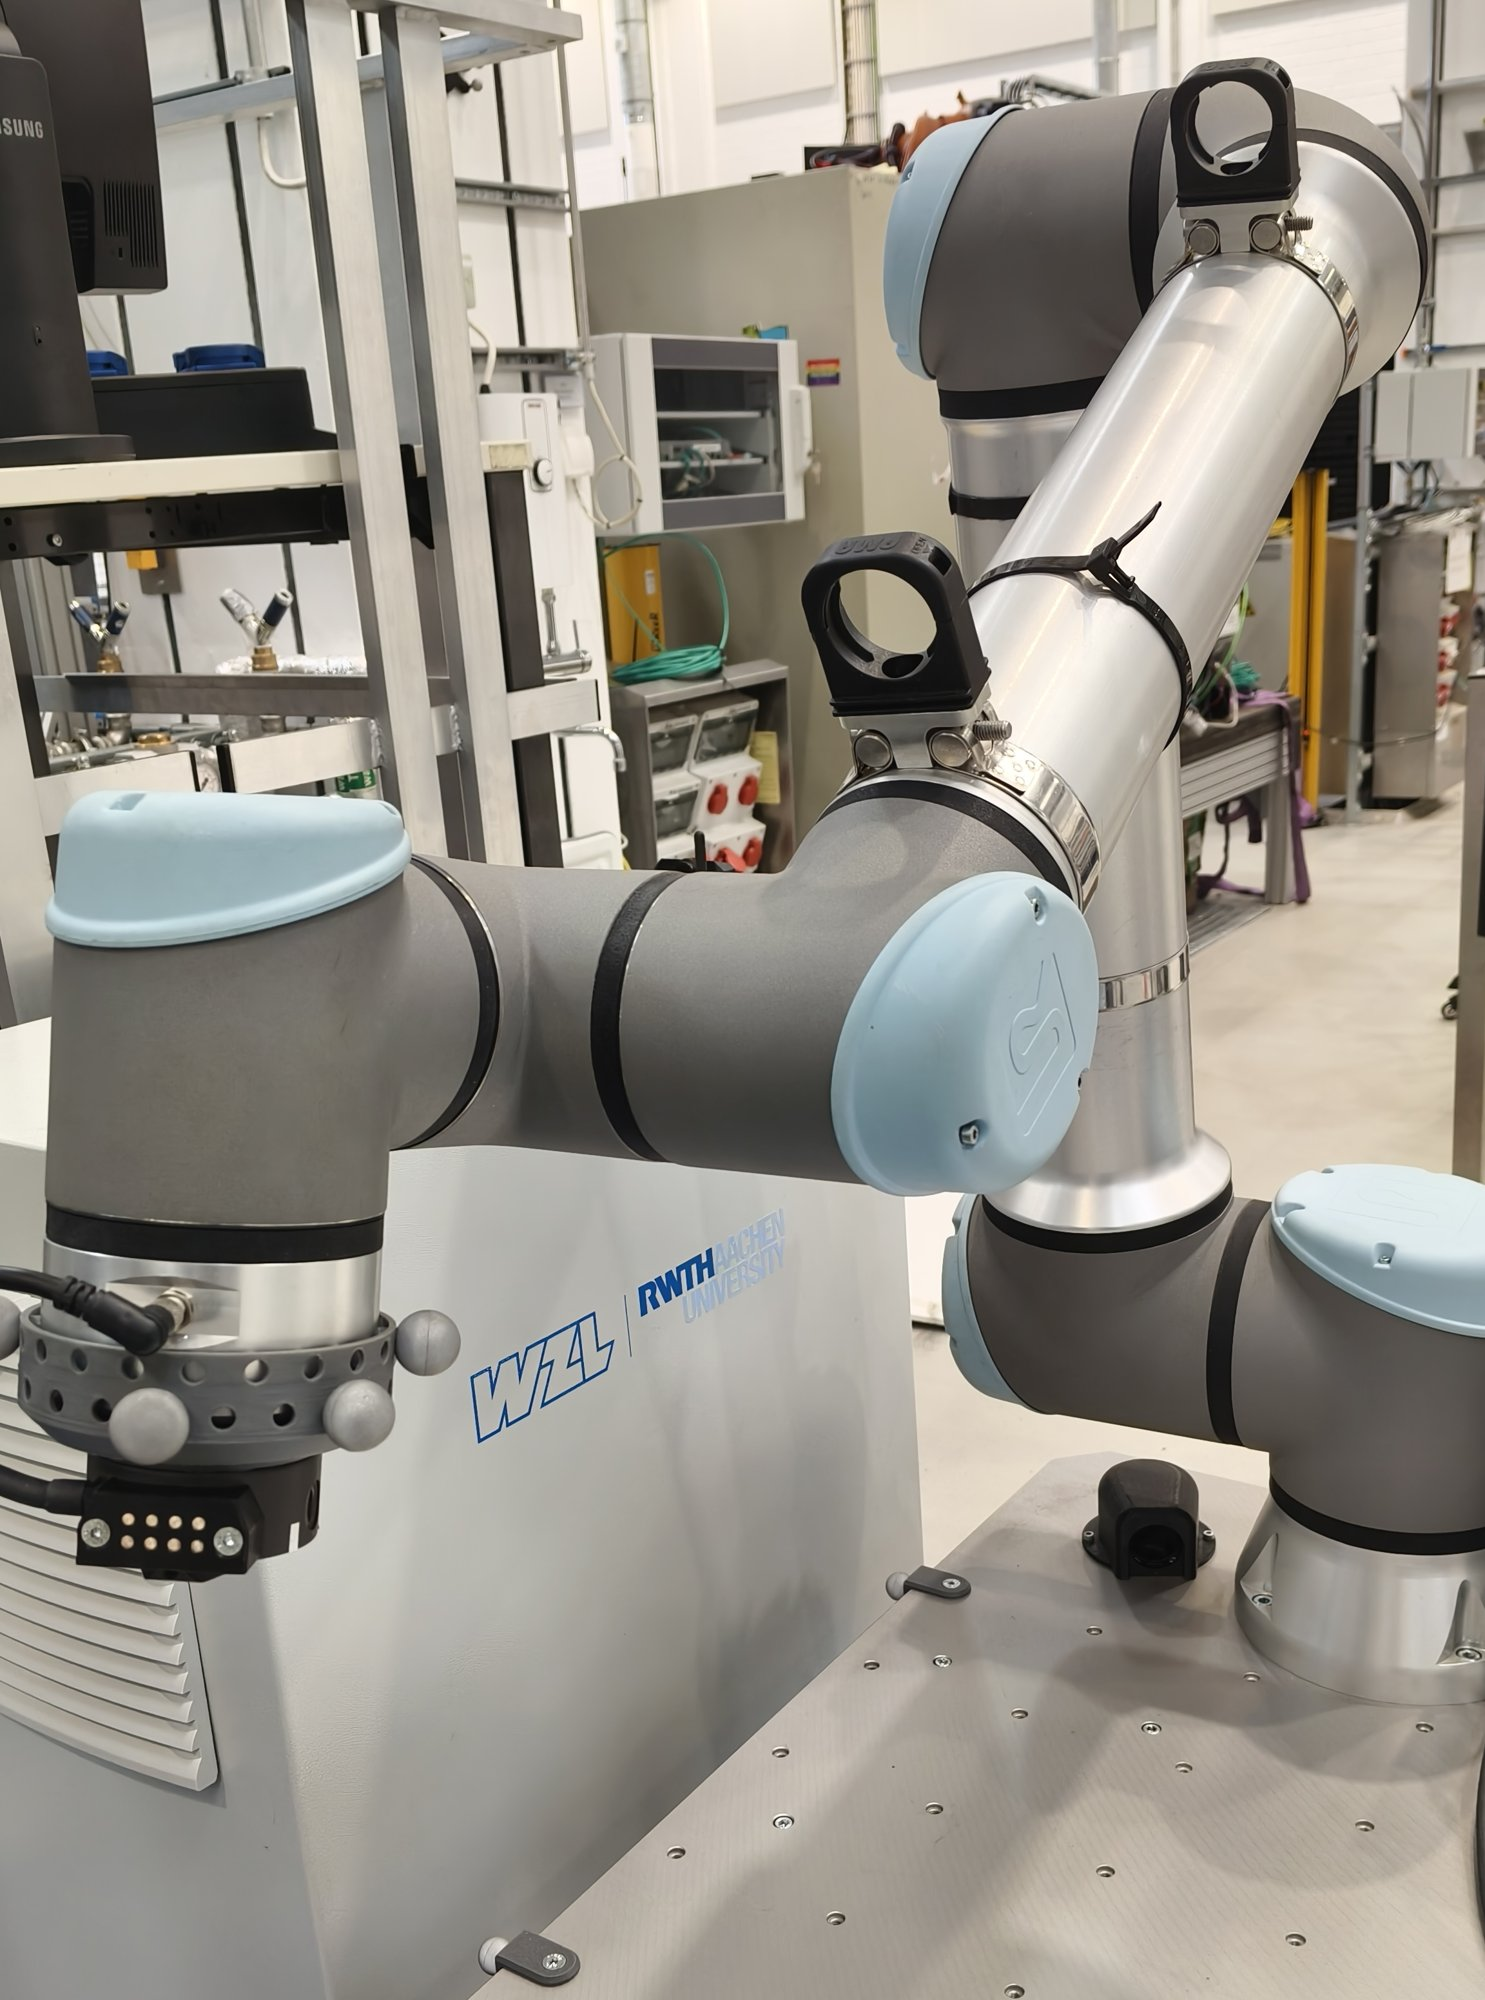
\includegraphics[height=5cm]{hero_tube_holders.jpg}
    \caption{Tube holders on the upper arm and the forearm.}
    \label{fig:collision-photo-tubes}
  \end{subfigure}
  \hfill
  \begin{subfigure}[t]{0.27\textwidth}
    \centering
    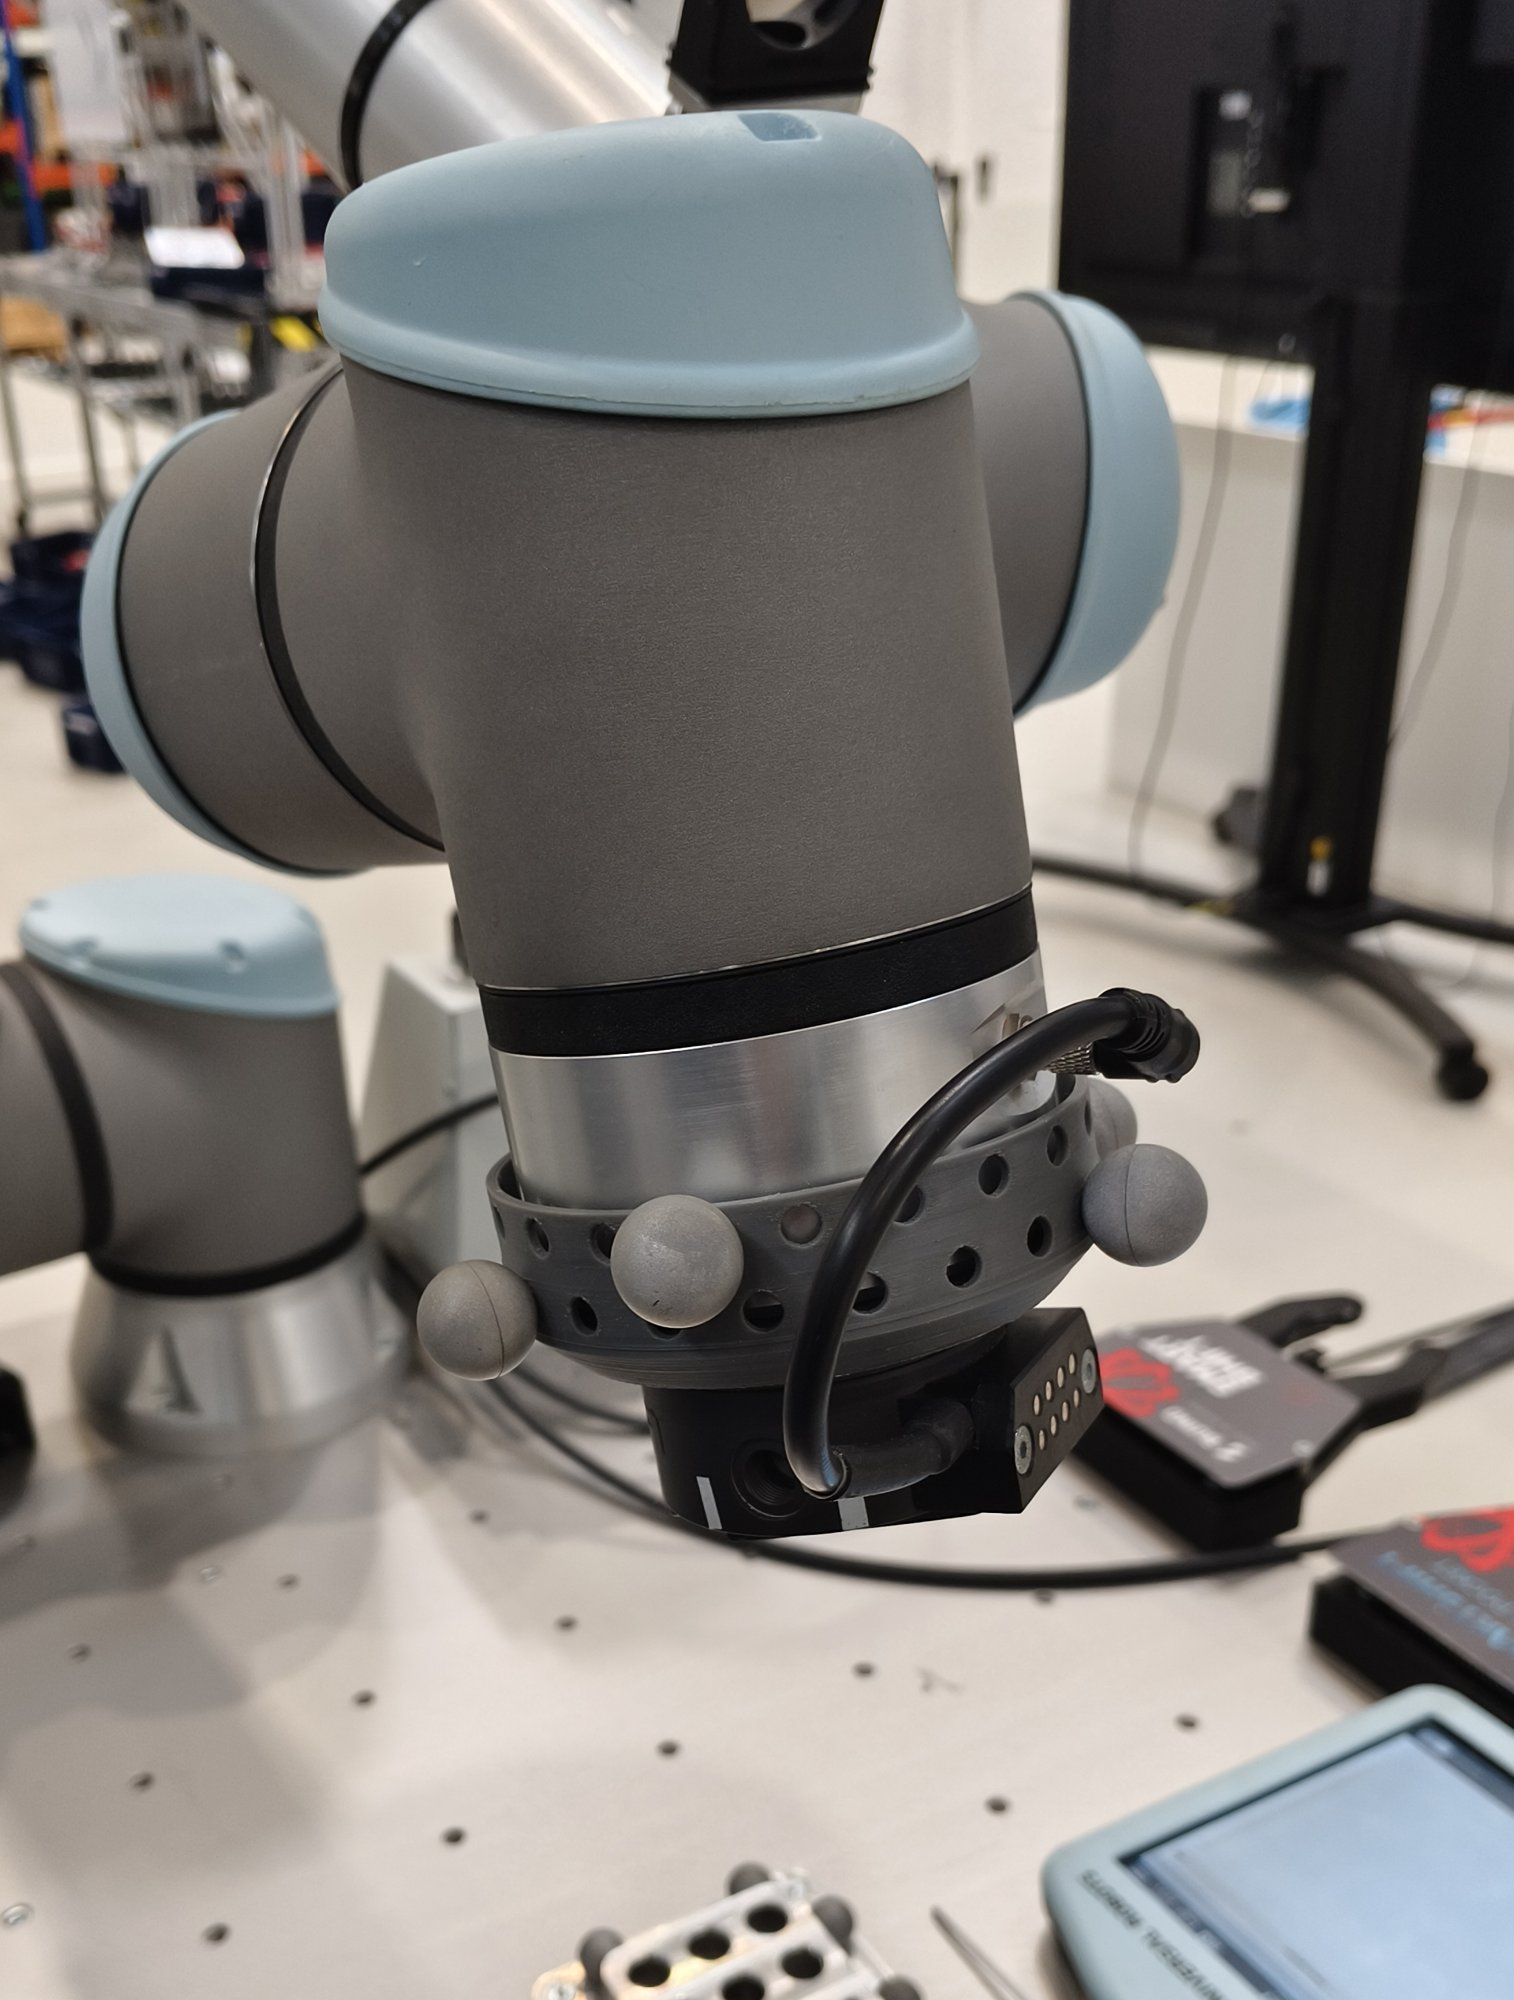
\includegraphics[height=5cm]{hero_tool_flange.jpg}
    \caption{Wrist~3 with the tool flange (\texttt{tool0}) and
      motion-capture markers.}
    \label{fig:collision-photo-flange}
  \end{subfigure}
  \caption{Platform bodies and arm attachments that enter the
    self-collision model.}
  \label{fig:collision-photos}
\end{figure}

The reduction to twelve pairs, listed in \cref{tab:collision-pairs},
removes pairs that are redundant rather than pairs that are harmless. An
attachment is dropped when the pair formed by its parent link and the
same platform body already keeps it clear. For the rings this holds with
any margin larger than their protrusion. For the tube holders it
required raising the minimum distance from \qty{0.08}{\meter} to
\qty{0.11}{\meter}, which leaves a clearance of about
\qty{5}{\centi\meter} for a dropped holder in its least favourable
orientation. The two largest holders sit on the forearm, the link that
most often dips towards the chassis during operation, and their pairs
with the chassis are kept explicitly. The dropped pairs are listed in a
comment of the task file but are not part of the model. Their effect on
solve time was not measured in isolation; the reduction cut the number
of distance queries per solve by \qty{62.5}{\percent}, and the UR safety
layer remains the last line of protection against a contact the reduced
set does not see.

\begin{table}[htbp]
  \centering
  \caption[Self-collision pairs before and after the reduction]{%
    Self-collision pairs between the arm and the two platform bodies,
    before (32) and after (12) the reduction. A dropped pair is covered
    by the pair of its parent link with the same platform body and the
    minimum distance of \qty{0.11}{\meter}.}
  \label{tab:collision-pairs}
  \begin{tabularx}{\linewidth}{@{}Xlcc@{}}
    \toprule
    Arm-side body & Protrusion & \texttt{hmi} & \texttt{chassis} \\
    \midrule
    \texttt{upper\_arm}, \texttt{forearm}, \texttt{wrist\_1}--\texttt{3}
      & link itself & kept (5) & kept (5) \\
    marker rings \texttt{ring2}, \texttt{ring2b}, \texttt{ring3}--\texttt{ring6}
      & $\le \qty{1}{\centi\meter}$ & dropped (6) & dropped (4) \\
    tube holders \texttt{bottom\_1}--\texttt{4}
      & \qtyrange{3}{6}{\centi\meter} & dropped (4) & dropped (4) \\
    tube holders \texttt{top\_3}, \texttt{top\_4} (forearm)
      & \qtyrange{3}{6}{\centi\meter} & dropped (2) & kept (2) \\
    \midrule
    Pairs before / after & & 17 / 5 & 15 / 7 \\
    \bottomrule
  \end{tabularx}
\end{table}

\Cref{fig:selfcollision-postures} shows two arm postures in which the
wrist comes close to the chassis. In both, the elbow is raised and the
forearm points downwards. In the first posture the three wrist links
arrive at the edge of the chassis top. In the second the forearm reaches
past that edge, and the wrist links lie beside the side wall of the
chassis, below the top plate. The pairs concerned are those of
\texttt{chassis} with \texttt{forearm\_link} and with
\texttt{wrist\_1\_link} to \texttt{wrist\_3\_link}.

\begin{figure}[htbp]
  \centering
  \begin{subfigure}[t]{0.544\textwidth}
    \centering
    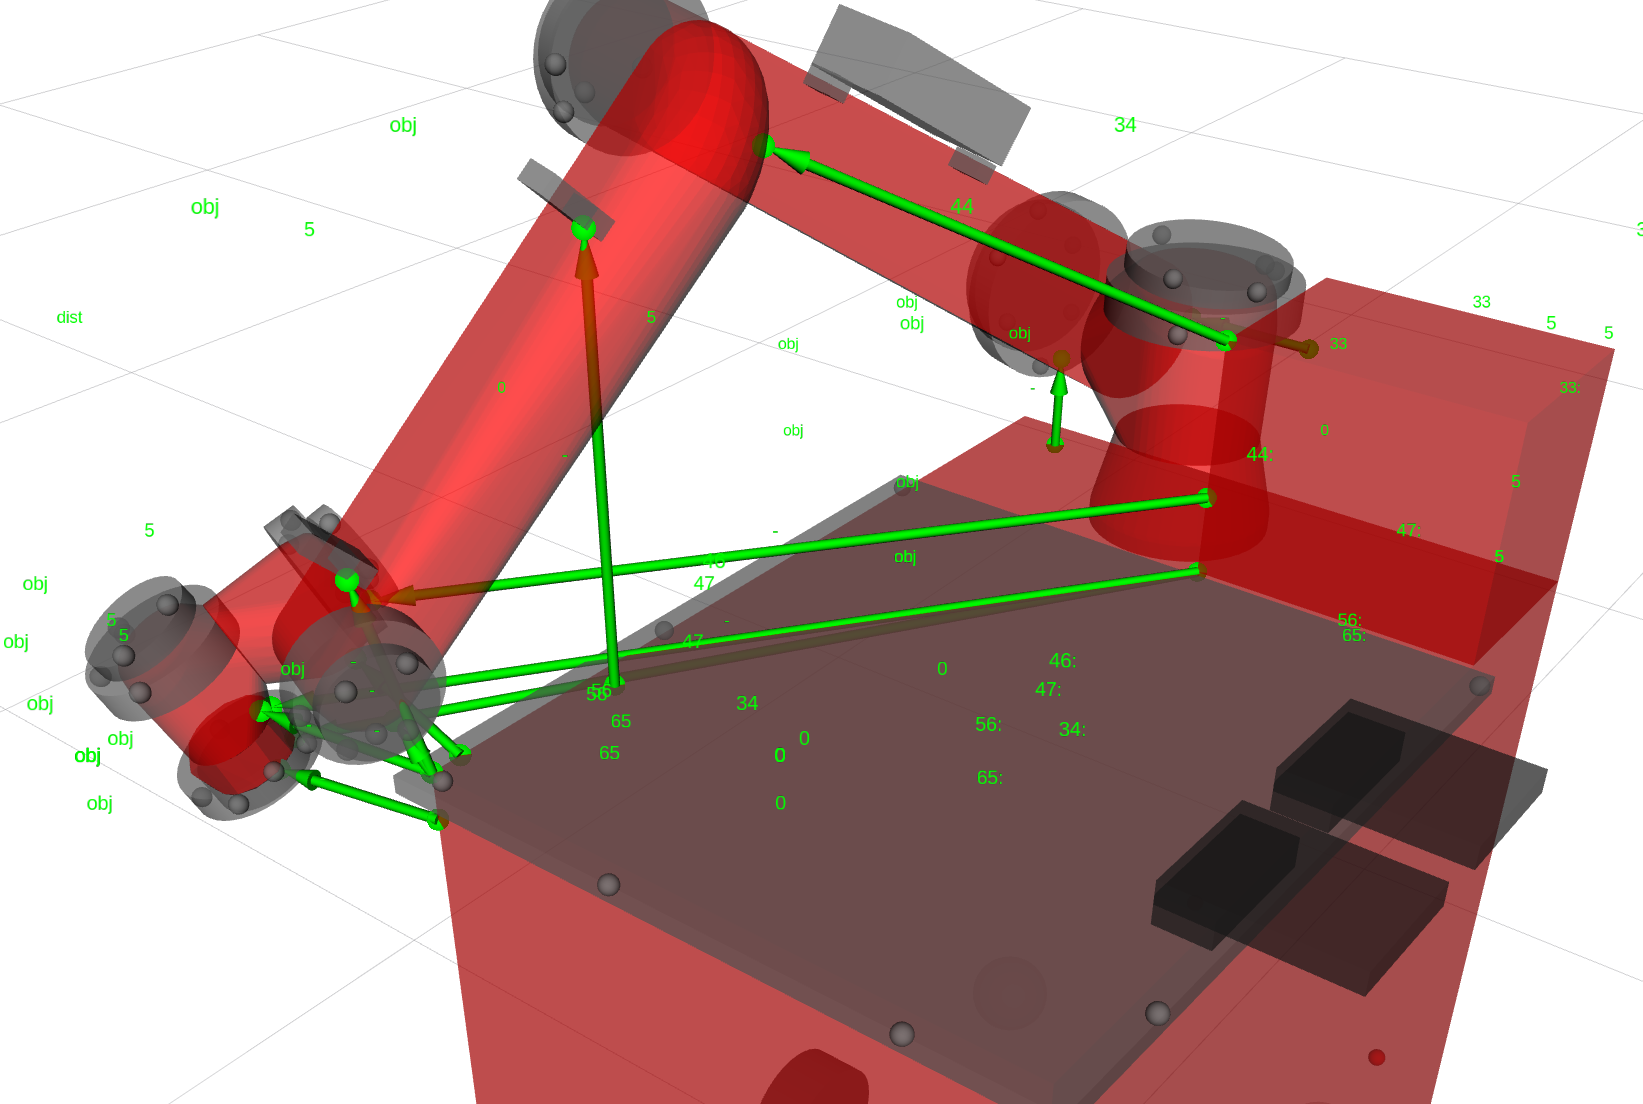
\includegraphics[width=\textwidth]{selfcollision_wrist_plate_edge.png}
    \caption{Wrist links at the edge of the chassis top}
    \label{fig:selfcollision-plate-edge}
  \end{subfigure}
  \hfill
  \begin{subfigure}[t]{0.436\textwidth}
    \centering
    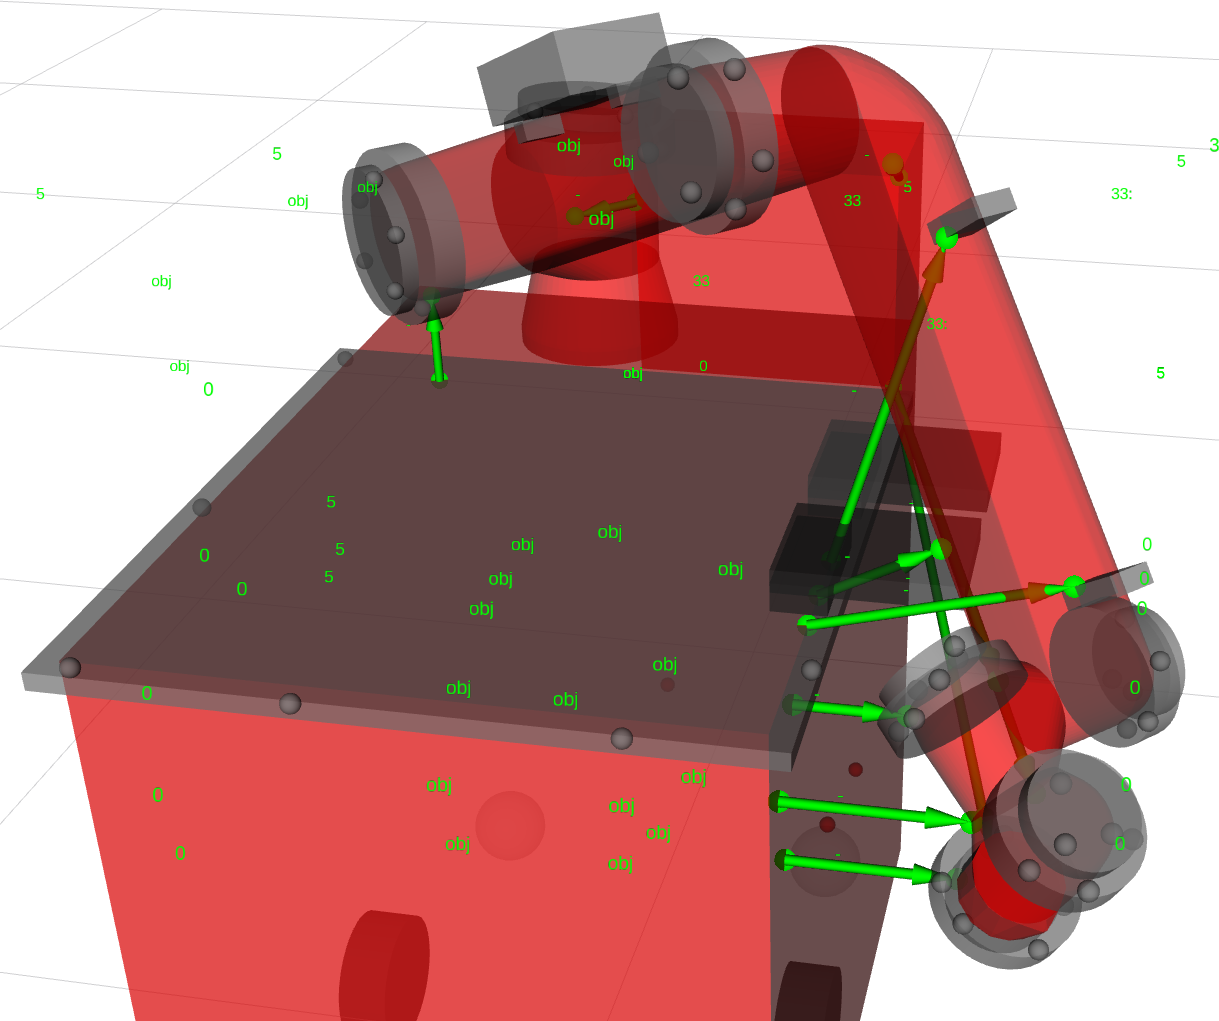
\includegraphics[width=\textwidth]{selfcollision_wrist_side_wall.png}
    \caption{Wrist links beside the side wall of the chassis}
    \label{fig:selfcollision-side-wall}
  \end{subfigure}
  \caption[Arm postures in which the wrist comes close to the chassis]{%
    Arm postures in which the wrist comes close to the chassis, drawn
    with the collision bodies of the model in RViz. Red bodies are the
    chassis, the operator panel (\texttt{hmi}) and the arm links; marker
    rings and tube holders are grey. Each green arrow joins the closest
    points of one body pair that the distance node evaluates. The green
    text is the label output of that node and is not evaluated here.}
  \label{fig:selfcollision-postures}
\end{figure}

The solver settings and the horizon are collected in
\cref{tab:mpc-config}. Three of them interact and are worth spelling
out. Only one SLQ iteration per solve is allowed. The solver starts a
new solve as soon as the previous one has finished
(\cref{sec:hw-interfaces}), so the previous solution, computed a few
hundred milliseconds earlier over a \qty{1.2}{\second} horizon, is a
usable initial guess; a second iteration would roughly double the solve
time and delay the next fresh observation by the same
amount~\cite{Farshidian2017SLQ}. The policy that the solver
publishes is declared valid for a \emph{solution time window} of
\qty{1.0}{\second}, shorter than the horizon; the bridge holds the robot
once a policy is exhausted rather than extrapolating it
(\cref{sec:hw-interfaces}). Real-time operation therefore requires

\begin{equation}
  2 \cdot \overline{t}_\mathrm{solve} \;<\; T_\mathrm{sol} \;<\; T ,
  \label{eq:rt-invariant}
\end{equation}

with $\overline{t}_\mathrm{solve}$ the average solve time,
$T_\mathrm{sol}$ the solution time window and $T$ the horizon: a policy
must arrive before the previous one expires, and it must not claim
validity beyond the horizon it was computed for. This invariant is
checked from the solver's diagnostics topic at the start of every
session and is the quantity that governs the failure mode analysed in
\cref{sec:hw-challenges}. \Cref{fig:rt-invariant} places the three
quantities on one time axis.

\begin{figure}[htbp]
  \centering
  \begin{tikzpicture}[
      font=\footnotesize,
      lbl/.style={font=\scriptsize, align=center},
      note/.style={font=\scriptsize, align=left},
      bar/.style={draw, minimum height=5.5mm, inner sep=0pt, anchor=west},
      tick/.style={thin, gray, dashed},
    ]
    % scale: 1 s = 6.5 cm
    \def\sT{7.8}    % horizon 1.2 s
    \def\sS{6.5}    % solution time window 1.0 s
    \def\sQ{3.0}    % 2 * average solve time, illustrative

    % --- guide lines --------------------------------------------------
    \draw[tick] (\sS,0.55) -- (\sS,-3.3);
    \draw[tick] (\sT,0.55) -- (\sT,-3.3);

    % --- bars ----------------------------------------------------------
    \node[bar, minimum width=\sT cm, fill=RWTHBlau100!12] (h) at (0,0) {};
    \node[lbl] at (\sT/2,0) {horizon $T = \qty{1.2}{\second}$};

    \node[bar, minimum width=\sS cm, fill=RWTHBlau100!25] (s) at (0,-1.0) {};
    \node[lbl] at (\sS/2,-1.0)
      {solution time window $T_\mathrm{sol} = \qty{1.0}{\second}$};

    \node[bar, minimum width=\sQ cm, fill=RWTHOrange100!30] (q) at (0,-2.0) {};
    \node[lbl] at (\sQ/2,-2.0) {$2\,\overline{t}_\mathrm{solve}$};

    % --- axis ----------------------------------------------------------
    \draw[-{Latex[length=1.8mm]}] (0,-3.0) -- (\sT+0.9,-3.0)
      node[right, font=\scriptsize] {$\tau$};
    \foreach \x/\t in {0/0} {
      \draw (\x,-2.9) -- (\x,-3.1) node[below, lbl] {\t};
    }
    \draw (\sS,-2.9) -- (\sS,-3.1) node[below, lbl] {$T_\mathrm{sol}$};
    \draw (\sT,-2.9) -- (\sT,-3.1) node[below, lbl] {$T$};

    % --- violation annotations ------------------------------------------
    \node[note, anchor=north west, text width=112mm] at (0,-3.55)
      {If $2\,\overline{t}_\mathrm{solve}$ reaches past $T_\mathrm{sol}$, a
       policy expires before its successor arrives and the bridge holds.
       If $T_\mathrm{sol}$ passed $T$, a policy would claim validity
       beyond the horizon it was computed for.};
  \end{tikzpicture}
  \caption[Real-time invariant of the \mpc{}--MRT loop]{%
    The three quantities of \cref{eq:rt-invariant} on one time axis, at
    the everyday operating point of \cref{tab:mpc-config}. The ordering
    $2\,\overline{t}_\mathrm{solve} < T_\mathrm{sol} < T$ is a design
    condition checked before a session, not a measurement, and the length
    of the $2\,\overline{t}_\mathrm{solve}$ bar is illustrative; the solve
    times actually reached on the two plants are reported in
    \cref{sec:hw-challenges}, where the \mpc{} loop runs at the wider
    Experiment~A setting.}
  \label{fig:rt-invariant}
\end{figure}

\begin{table}[!htbp]
  \centering
  \caption[\ocs{} operating point on \hero{}]{%
    \ocs{} operating point for on-robot operation, as configured in
    \texttt{task\_hardware.info}. Velocity limits appear twice by
    design: once as a soft constraint inside the optimisation and once
    as a hard clamp in the bridge.}
  \label{tab:mpc-config}
  \begin{tabularx}{\linewidth}{@{}lXl@{}}
    \toprule
    Group & Parameter & Value \\
    \midrule
    Model    & state / input dimension        & $9$ / $8$ \\
             & base frame, \ee{} frame        & \texttt{footprint}, \texttt{tool0} \\
             & fixed joints                   & both wheel joints \\
    \addlinespace
    Solver   & algorithm                      & SLQ \\
             & iterations per solve           & $1$ \\
             & threads                        & $8$ \\
             & backward-pass step, integrator & \qty{2}{\milli\second}, ODE45 \\
             & rollout step                   & \qty{10}{\milli\second} \\
             & feedback policy                & disabled (feed-forward) \\
    \addlinespace
    \mpc{}   & horizon $T$                    & \qty{1.2}{\second} \\
             & solution time window $T_\mathrm{sol}$ & \qty{1.0}{\second} \\
             & bridge loop rate $f_\mathrm{MRT}$ (\texttt{mrtDesiredFrequency}) & \qty{50}{\hz} \\
             & solve rate                     & $\min(f_\mathrm{MRT},\, 1/t_\mathrm{solve})$ \\
             & \texttt{mpcDesiredFrequency}   & \qty{10}{\hz}, warning threshold only \\
    \addlinespace
    Cost     & $R_\mathrm{base}$, $R_\mathrm{arm}$ & $0.085\,I_2$, $0.04\,I_6$ \\
             & $\mu_\mathrm{p}$, $\mu_\mathrm{o}$ (running and final) & $10$, $5$ \\
    \addlinespace
    Limits   & base velocity                  & \qty{\pm 0.1}{\meter\per\second}, \qty{\pm 0.1}{\radian\per\second} \\
             & arm joint velocity             & \qty{\pm 0.3}{\radian\per\second} \\
             & arm joint positions           & UR safety-panel limits \\
             & self-collision pairs, margin   & $12$, \qty{0.11}{\meter} \\
    \bottomrule
  \end{tabularx}
\end{table}

Derivatives are not written by hand. \ocs{} traces the cost terms, the
constraints and the system equation with CppAD and compiles the
resulting derivative code into shared libraries on first use, which is
the delay mentioned in
\cref{sec:distributed-arch}~\cite{CppAD,ocs2Toolbox}. The cache is keyed
by the model, not by the tuning: changing the kinematic model, the fixed
joints or the collision pair list invalidates it and requires a
regeneration, whereas changing a weight, a limit or the horizon takes
effect on the next restart. This distinction matters in practice,
because a stale cache silently keeps the old model while the
configuration file suggests otherwise.

% ---------------------------------------------------------------------
\section{Hardware Interfaces and ROS Control Layer Integration}
\label{sec:hw-interfaces}

The MRT bridge is the only component written specifically for this
deployment. It is the MRT client of the MPC--MRT split
(\cref{sec:sota-ocs2}) adapted to the real robot, and it closes the loop
between the \ocs{} policy and \texttt{ros2\_control} on the
IPC~\cite{ros2control}. Its practical role is to decouple the actuation
rate from the solve rate. A policy arrives only every few hundred
milliseconds, but it is a function of time over the solution time
window, so the bridge can evaluate it at the current time in every cycle
and keep commanding the robot between solves. The bridge is also the
place where a policy that has become too old is detected and replaced
by a hold.

The bridge has a single clock, the loop rate $f_\mathrm{MRT}$ set by
\texttt{mrtDesiredFrequency} in the task file. Each cycle publishes an
observation, collects a newly arrived policy, runs the checks of
\cref{tab:bridge-guards} and evaluates the policy into a base twist and
an arm setpoint. The observation also paces the solver: the \mpc{} node
solves inside the callback of each observation it receives, with a queue
depth of one and no throttle of its own~\cite{ocs2Toolbox}. The solve
rate on the robot is therefore $\min(f_\mathrm{MRT}, 1/t_\mathrm{solve})$,
with $t_\mathrm{solve}$ the duration of one solve. The
\texttt{mpcDesiredFrequency} entry of \qty{10}{\hz} does not throttle
anything on this path; the bridge uses it only as the warning threshold
in \cref{tab:bridge-guards}.

The loop rate was lowered from \qty{100}{\hz} to \qty{50}{\hz} after the
sessions reported in \cref{ch:hardware}, which ran at \qty{100}{\hz}.
At \qty{100}{\hz} the bridge sampled the base faster than its state
source changes: the drive controller publishes odometry at
\qty{50}{\hz}, so every second observation carried the same base pose
as the one before it. That doubled the observation traffic over the
network and the work of the bridge on the four-thread IPC without adding
information. The solver was not affected, because with solves of a few
hundred milliseconds it runs back to back at either rate. The lower rate
keeps the other requirements on the loop satisfied with margin. The base
twist is held for one cycle, which at the \qty{0.1}{\meter\per\second}
bound is a step of \qty{2}{\milli\meter} instead of
\qty{1}{\milli\meter}. The \qty{0.2}{\second} staleness window is still
checked ten times, and the \qty{0.5}{\second} command timeout of the
drive controller spans 25 cycles. The commanded arm speed is bounded by
the step clamp described below, independently of the loop rate. The
price is that a new policy may wait up to one cycle,
\qty{20}{\milli\second}, before it is first used.

Each cycle begins with an observation. The base pose $(p_x, p_y, \psi)$
is taken from the drive controller's odometry, with the yaw extracted
from the reported quaternion, and $\qarm$ is looked up by joint name in
\texttt{/joint\_states}; a missing joint aborts the cycle with a
throttled warning instead of silently inserting a zero. The observation
timestamp is the later of the two message stamps, expressed relative to
the origin fixed at the first accepted measurement, which is the
relative time axis that makes the deployment insensitive to clock
offsets.

Before the first command, the bridge performs a reset handshake with the
\mpc{} node. The initial reference must not move the robot, so the
bridge computes the current \ee{} pose by forward kinematics from the
latest observation and sends it as a two-knot target trajectory inside
the reset request: the solver starts by holding the pose the robot is
already in. The bridge guards the handshake against both ways it can
fail. It waits for
the reset service rather than assuming it exists, logs an actionable
error after \qty{15}{\second} and keeps waiting, and retries the request
if the response is lost---a single dropped reply over the network must
not leave the bridge dead. After a handshake the time-axis baseline is
reset as well, because the blocking call may have consumed several
seconds and the next observation would otherwise look like a time jump.
\Cref{fig:reset-handshake} shows the exchange and the two ways it can
fail.

\begin{figure}[htbp]
  \centering
  \begin{tikzpicture}[
      font=\footnotesize,
      head/.style={draw, rounded corners=1pt, align=center, inner sep=3.5pt,
                   minimum height=7mm, minimum width=36mm},
      life/.style={dashed, gray},
      msg/.style={-{Latex[length=2mm]}, thick},
      selfact/.style={draw, rounded corners=1pt, align=left, inner sep=3pt,
                      font=\scriptsize, fill=gray!10},
      lbl/.style={font=\scriptsize, align=center},
      note/.style={font=\scriptsize, align=left, text=RWTHOrange100},
    ]
    \node[head] (b) at (0,0)   {MRT bridge (IPC)};
    \node[head] (m) at (8.2,0) {\mpc{} node (external PC)};
    \draw[life] (b.south) -- (0,-7.3);
    \draw[life] (m.south) -- (8.2,-7.3);

    % --- 1: build the initial target --------------------------------
    \node[selfact, anchor=west] (a1) at (0.25,-1.15)
      {forward kinematics of the latest observation\\
       $\rightarrow$ two-knot target at the current \ee{} pose};

    % --- 2: probe the service ---------------------------------------
    \node[selfact, anchor=west] (a2) at (0.25,-2.5)
      {probe \texttt{\dots\_mpc\_reset}, one attempt per second};
    \node[note, anchor=east, align=right, text width=30mm] at (-0.3,-2.5)
      {after \qty{15}{\second}: actionable\\error, and keep waiting};

    % --- 3: request ---------------------------------------------------
    \draw[msg] (0,-3.7) -- (8.2,-3.7)
      node[lbl, midway, above] {reset request, target in the payload};

    % --- 4: solver resets --------------------------------------------
    \node[selfact, anchor=east] (a4) at (7.95,-4.6)
      {reset the solver; write the target\\into the reference manager};

    % --- 5: response ---------------------------------------------------
    \draw[msg] (8.2,-5.6) -- (0,-5.6)
      node[lbl, midway, above] {response};
    \node[note, anchor=east, align=right, text width=30mm] at (-0.3,-5.6)
      {response lost: hold and\\retry on the next cycle};

    % --- 6: baseline --------------------------------------------------
    \node[selfact, anchor=west] (a6) at (0.25,-6.6)
      {clear the time-axis baseline; handshake done};
  \end{tikzpicture}
  \caption[Reset handshake between the MRT bridge and the \mpc{} node]{%
    Reset handshake that precedes the first command. The bridge derives
    the initial reference from its own latest observation, so the solver
    starts by holding the pose the robot is already in. Both guards, in
    orange, sit in the bridge: it waits for the service rather than
    assuming it exists, and a lost response leaves it holding and
    retrying instead of dead. Clearing the time-axis baseline
    afterwards is necessary because the blocking call may have consumed
    several seconds, which the next observation would otherwise present as
    a time jump.}
  \label{fig:reset-handshake}
\end{figure}

The base command is the first two elements of the optimised input,
published as a stamped twist on \texttt{/cmd\_vel\_ocs2} rather than
directly on the drive controller's command topic. A \texttt{twist\_mux}
arbitrates between sources by priority, with manual teleoperation above
\ocs{}, so a higher-priority teleoperation source preempts or stops a
\qty{400}{\kilo\gram} platform that is executing an optimised
trajectory~\cite{twistMux}. The published twist is clamped to the same
base velocity bounds that the optimisation uses as a soft constraint; the
clamp is the hard backstop for the case where the soft constraint is
violated.

The arm command needs additional handling, because the joint-trajectory
controller accepts a position setpoint over its topic interface without
enforcing any velocity limit~\cite{ros2control}. The bridge samples the
optimised arm state \qty{0.6}{\second} ahead and publishes it as a single
trajectory point with that time from start, but it first clamps each
joint's step to
$\dot{q}_\mathrm{max} \cdot t_\mathrm{preview} = \qty{0.18}{\radian}$
around the currently measured position. Because the next cycle repeats
the computation \qty{20}{\milli\second} later, the arm still advances
towards the target, at a rate bounded by
\qty{0.3}{\radian\per\second}. When the clamp engages, the bridge warns;
frequent warnings indicate that the optimised state is jumping between
solves, which later proved useful as a diagnostic and is taken up in
\cref{sec:hw-challenges}.

Whenever the bridge cannot produce a trustworthy command it publishes a
hold: a zero twist and an arm trajectory pinned at the measured joint
positions. Getting this right required two details that are invisible in
the algorithm but decide whether the robot actually stops. The twist is
stamped at the moment of publication, because a hold issued right after
a blocking call would otherwise carry a stale stamp and be rejected by
the drive controller as timed out. The arm trajectory carries a zero
header stamp, which the controller reads as ``start now''; a wall-clock
stamp arrives a few milliseconds late and the whole trajectory is
rejected as ending in the past, so the hold never applies.
\Cref{tab:bridge-guards} lists the conditions that trigger a hold, and
\cref{fig:bridge-cycle} places them in the order the cycle evaluates
them.

\begin{figure}[htbp]
  \centering
  \begin{tikzpicture}[
      font=\footnotesize,
      act/.style={draw, rounded corners=1pt, align=center, inner sep=3.5pt,
                  minimum height=8mm, minimum width=56mm},
      guard/.style={act, fill=gray!10},
      hold/.style={act, draw=RWTHOrange100, thick, minimum width=22mm},
      cmd/.style={act, minimum width=40mm},
      flow/.style={-{Latex[length=2mm]}, thick},
      rail/.style={thick},
      lbl/.style={font=\scriptsize, align=center},
      side/.style={font=\scriptsize, align=left},
    ]
    % --- main column -------------------------------------------------
    \node[act]   (obs) at (0,0)
      {observation from odometry and \texttt{/joint\_states},\\
       stamped with the later of the two};
    \node[guard] (g1)  at (0,-1.6) {measurement age $> \qty{0.2}{\second}$?};
    \node[guard] (g2)  at (0,-2.9)
      {$\Delta t < 0$ or $\Delta t > \qty{0.5}{\second}$?};
    \node[guard] (g3)  at (0,-4.2) {reset handshake done?};
    \node[act]   (upd) at (0,-5.5)
      {publish the observation, fetch the latest policy\\
       (no policy received yet: end the cycle)};
    \node[guard] (g4)  at (0,-6.8) {no new policy for $2\,T_\mathrm{sol}$?};
    \node[guard] (g5)  at (0,-8.1) {remaining policy validity $\le 0$?};
    \node[act]   (ev)  at (0,-9.4)
      {evaluate the policy at \texttt{observation.time}\\
       $\rightarrow$ input $\uvec$, state $\svec$};
    \node[cmd]   (base) at (-2.6,-11.3)
      {clamp $v, \omega$ to $\pm 0.1$;\\
       stamp at publication\\
       $\rightarrow$ \texttt{twist\_mux}};
    \node[cmd]   (arm)  at (2.6,-11.3)
      {clamp the step to $\pm \qty{0.18}{\radian}$,\\
       then to the panel limits\\
       $\rightarrow$ joint-trajectory controller};

    % --- hold ---------------------------------------------------------
    \node[hold] (hd) at (6.2,-4.85) {hold};
    \node[side, anchor=north west, text width=21mm] at (5.15,-5.45)
      {no policy for $5\times$ the timeout: also re-arm the handshake};

    % --- main flow ----------------------------------------------------
    \draw[flow] (obs) -- (g1);
    \draw[flow] (g1)  -- (g2)  node[lbl, midway, left=1mm] {no};
    \draw[flow] (g2)  -- (g3)  node[lbl, midway, left=1mm] {no};
    \draw[flow] (g3)  -- (upd) node[lbl, midway, left=1mm] {yes};
    \draw[flow] (upd) -- (g4);
    \draw[flow] (g4)  -- (g5)  node[lbl, midway, left=1mm] {no};
    \draw[flow] (g5)  -- (ev)  node[lbl, midway, left=1mm] {no};
    \draw[flow] (0,-9.85) -- (0,-10.3) -| (base.north);
    \draw[flow] (0,-9.85) -- (0,-10.3) -| (arm.north);

    % --- guard exits to the hold rail ---------------------------------
    \draw[rail] (g1.east) -- (4.9,-1.6) node[lbl, pos=0.4, above] {yes};
    \draw[rail] (g4.east) -- (4.9,-6.8) node[lbl, pos=0.4, above] {yes};
    \draw[rail] (g5.east) -- (4.9,-8.1) node[lbl, pos=0.4, above] {yes};
    \draw[rail] (4.9,-1.6) -- (4.9,-8.1);
    \draw[flow] (4.9,-4.85) -- (hd.west);

    % --- left-hand exits ----------------------------------------------
    \draw[rail] (g2.west) -- (-4.6,-2.9) node[lbl, pos=0.35, above] {yes};
    \node[side, anchor=south east, text width=33mm] at (-4.6,-2.78)
      {drop the frame; after 20 in a row, re-baseline the time axis and
       re-handshake};
    \draw[rail] (g3.west) -- (-4.6,-4.2) node[lbl, pos=0.35, above] {no};
    \node[side, anchor=north east, text width=33mm] at (-4.6,-4.32)
      {run the handshake of \cref{fig:reset-handshake}; on success
       continue, on failure hold};
  \end{tikzpicture}
  \caption[One cycle of the MRT bridge]{%
    One cycle of the MRT bridge, which runs at \qty{50}{\hz} on the IPC.
    The guards are evaluated in the order shown; each either passes the
    cycle on or ends it in the hold, which publishes a zero twist stamped
    at publication together with an arm trajectory pinned at the measured
    positions under a zero header stamp. The arm step limit of
    \qty{0.18}{\radian} is the product of the arm velocity bound and the
    preview time, \qty{0.3}{\radian\per\second} $\times$
    \qty{0.6}{\second}, so the arm still advances towards the optimised
    state over successive cycles. Thresholds and their origin are listed
    in \cref{tab:bridge-guards}.}
  \label{fig:bridge-cycle}
\end{figure}

\begin{table}[htbp]
  \centering
  \caption[Guards implemented in the MRT bridge]{%
    Guards implemented in the MRT bridge. Most thresholds are launch
    arguments of the bridge; the policy timeout is derived from
    $T_\mathrm{sol}$, and the warning threshold from
    \texttt{mpcDesiredFrequency}, both in the task configuration file.}
  \label{tab:bridge-guards}
  \begin{tabularx}{\linewidth}{@{}lX@{}}
    \toprule
    Condition & Reaction \\
    \midrule
    Measurement older than \qty{0.2}{\second}
      & hold; the state estimate is not trusted \\
    Observation time steps backwards, or forwards by more than
    \qty{0.5}{\second}
      & drop the frame to protect the solver's time axis; after $20$
        consecutive drops, accept the new time as baseline and
        re-handshake \\
    Remaining policy validity below \qty{0.1}{\second}
      ($1/\texttt{mpcDesiredFrequency}$)
      & warn: the robot is outrunning the optimiser \\
    Policy validity exhausted
      & hold instead of evaluating a policy beyond its window \\
    No new policy for $2\,T_\mathrm{sol}$, at least \qty{1}{\second}
      & hold; the external PC or the link is assumed busy \\
    No new policy for $5\times$ that time, at least \qty{5}{\second}
      & re-run the reset handshake, on the assumption that the \mpc{}
        node restarted and no longer accepts the current observations \\
    Commanded arm step beyond the rate limit
      & clamp the step and warn \\
    \bottomrule
  \end{tabularx}
\end{table}

Below the bridge, the control chain is the production \hero{} stack with
two deliberate deviations. The UR driver is started in headless mode
with the joint-trajectory controller active, so that whole-body control
does not depend on an operator starting a program on the teach pendant;
the trade-off is that the pendant must be in remote mode when the driver
starts, otherwise the external control program has to be re-sent. The
controller stopper, which deactivates arm controllers when no
program runs on the arm, keeps both the joint-trajectory controller and
the drive controller in its list of controllers to leave alone. This
preserves the safety interlock of the arm while ensuring that a
protective stop does not silently drop the controller through which
\ocs{} actuates.

Two limitations of the integration follow from the choices above rather
than from tuning, and both bound what the experiments in the following
chapters can show. The controller's notion of where the robot is comes
from wheel odometry alone, so \ee{} poses reconstructed from the
internal state are consistent within a run but not absolute; and the
optimisation reasons about the robot's own geometry only, so a
whole-body plan is collision-free with respect to the platform and blind
to the workspace around it.

% !TeX root = ../main.tex
\chapter{Simulation-Based Validation}
\label{ch:simulation}

The hardware loop of \cref{ch:integration} mixes three contributions to
the recorded \ee{} error: the residual of the optimiser on its own
kinematic model, the lag and clamping of the MRT bridge, and the
odometry-plus-forward-kinematics estimate of where the robot is. A
kinematic closed loop that replaces the bridge with an ideal rollout
removes the last two, so a fault in the reference, the time axis or the
cost function can be seen before it is blamed on the plant. That loop is
the dummy MRT of \ocs{}. \Cref{sec:sim-methodology} states what it can
show and defines the metrics used here and in \cref{ch:hardware}.
\Cref{sec:sim-dummy} describes the closed \ee{} path that the dummy
exercises and the checks that a session must pass before the same files
are taken to the robot.

% ---------------------------------------------------------------------
\section{Validation Methodology and Evaluation Metrics}
\label{sec:sim-methodology}

The dummy MRT is not a second controller. It is the production \mpc{}
node and the production target publisher, closed through
\texttt{MRT\_ROS\_Dummy\_Loop} instead of the hardware bridge
(\cref{sec:hw-interfaces}). The dummy integrates the latest policy with
the same kinematic rollout the solver uses, at the configured MRT rate of
\qty{100}{\hz}, and feeds the resulting state back as the next
observation. There is no policy-evaluation lag, no actuator dynamics, and
no wheel-odometry drift. The \ee{} error that remains is the optimiser's
residual against its own model: input costs and velocity limits prevent a
perfect match to the interpolated reference, and a finite horizon cannot
see the whole path.

That residual is useful. If the dummy already leaves the commanded path,
the later hardware error is not an execution problem. If the dummy
tracks and the hardware does not, the gap is in the bridge, the
actuators, or the state estimate, which is the comparison drawn in
\cref{ch:hardware}. The dummy does not speak to real-time behaviour on
the IPC: solve time, policy exhaustion and the observation-age guard
never appear, because the observation is produced in the same process
tree as the solver.

A second simulated-hardware mode exists in the \hero{} stack: mock
\texttt{ros2\_control} interfaces that echo commands into states while
still running the MRT bridge~\cite{ros2control}. That mode keeps the
timing and clamping of \cref{sec:hw-interfaces} and is used as a
stepping stone onto the physical platform. It is not the subject of this
chapter.

\subsection{Internal metrology}
\label{sec:sim-metrology}

Desired and attained \ee{} poses are both computed inside the waypoint
node from the same \mpc{} observation. The desired pose is the linear
interpolation of the commanded knots at \texttt{observation.time}, which
is the interpolation \ocs{} itself uses for the position part of the
reference. The attained pose is Pinocchio forward kinematics of that
observation, with \texttt{tool0} as the \ee{} frame
(\cref{sec:hero-platform}). The error signal therefore carries no
cross-topic time-alignment residual. The node publishes it at
\qty{20}{\hz} on \texttt{/ee\_waypoint\_target/ee\_metrics}.

On the dummy this is a consistent kinematic measurement. On hardware the
same pipeline reconstructs the \ee{} from wheel odometry and joint
encoders. Drift of the base pose then contaminates every later metric.
The figures and tables of this chapter, and the internal traces of
\cref{ch:hardware}, are therefore internal metrology. An ISO-conforming
accuracy statement would require an external pose of the \ee{}, for
example from an OptiTrack system, with the uncertainty budget of
ISO~9283:1998 cl.~6.5~\cite{ISO9283}. That measurement is not part of
the present experiments.

\subsection{Time-aligned pose error}
\label{sec:sim-pose-error}

Let $\symbf{p}_\mathrm{d}(t)$ and $\symbf{p}_\mathrm{a}(t)$ be the
desired and attained positions in the \texttt{world} frame, and
$q_\mathrm{d}(t)$, $q_\mathrm{a}(t)$ the corresponding unit quaternions.
The position and orientation errors used throughout are
\begin{equation}
  e_{\mathrm{p}}(t) = \lVert \symbf{p}_\mathrm{d}(t) -
    \symbf{p}_\mathrm{a}(t) \rVert,
  \qquad
  e_{\mathrm{o}}(t) = 2\,\mathrm{atan2}\bigl(\lVert \symbf{v} \rVert,
    \lvert w \rvert\bigr),
  \label{eq:ee-errors}
\end{equation}
where $(w,\symbf{v})$ are the scalar and vector parts of
$q_\mathrm{d}\,q_\mathrm{a}^{-1}$ and $e_{\mathrm{o}}$ is folded into
$[0,\pi]$ so that the quaternion double cover does not appear as a
$2\pi$ jump. On a measured edge of the path the position error is split
into an along-track component $e_{\parallel} = \symbf{e}\cdot\symbf{\tau}$
and a cross-track remainder $e_{\perp} = \lVert \symbf{e} -
e_{\parallel}\,\symbf{\tau} \rVert$, with $\symbf{\tau}$ the unit
tangent of that edge. The ratio
\begin{equation}
  t_{\mathrm{lag}} = e_{\parallel} / v_{\mathrm{ref}}
  \label{eq:lag-eff}
\end{equation}
converts the along-track error into an equivalent time, with
$v_{\mathrm{ref}}$ the commanded path speed. On hardware,
$t_{\mathrm{lag}}$ is the quantity that can be compared with the
policy-lag diagnostic of the MRT bridge
(\cref{sec:hw-challenges}); the dummy has no such lag, so a large
$t_{\mathrm{lag}}$ there would mean the optimiser is chronically behind
its own reference.

These samples are only admitted on the measured path. The waypoint node
tags every metric with a segment identifier: \texttt{segment\_id} $\ge
1$ is an edge of the closed box; $0$ is the approach from the current
\ee{} to the entry point; $-10$, $-11$ and $-12$ are the lead-in,
lead-out and optional park legs of ISO~9283 cl.~8.2~\cite{ISO9283}.
Post-processing keeps $\texttt{segment\_id} \ge 1$. The transients of
starting, stopping and parking do not enter $e_{\mathrm{p}}$,
$t_{\mathrm{lag}}$ or the path metrics below.

\subsection{Path metrics: Hausdorff distance and ISO path accuracy}
\label{sec:sim-path-metrics}

Time-aligned error assumes that the commanded and attained poses share a
clock and a speed profile. That is true for the \ocs{} loop, where the
reference is a time-parameterised \texttt{TargetTrajectories} message.
It is not true of a decoupled Nav2 plus MoveIt baseline, which would
reach the same corners with a different velocity profile and with
pauses while the base repositions. A later comparison of the two
pipelines therefore needs a metric that treats the command as a
geometric path, not as a trajectory. The (symmetric) Hausdorff distance
between the commanded point set $A$ and the attained point set $B$ is
\begin{equation}
  h(A,B) = \max_{a \in A} \min_{b \in B} \lVert a-b \rVert,
  \qquad
  H(A,B) = \max\bigl(h(A,B),\, h(B,A)\bigr).
  \label{eq:hausdorff}
\end{equation}
The directed distance $h(B,A)$ is small whenever every attained sample
lies near the command, including the degenerate case of a robot that
stops halfway; $h(A,B)$ penalises shortcuts and unfinished laps. Both
directions are required. The classical $\max$ is sensitive to a single
spike, so results are reported as the symmetric mean
\begin{equation}
  \overline{H}(A,B)
    = \frac{1}{2|A|}\sum_{a\in A}\min_{b\in B}\lVert a-b \rVert
    + \frac{1}{2|B|}\sum_{b\in B}\min_{a\in A}\lVert a-b \rVert
  \label{eq:mean-hausdorff}
\end{equation}
together with the 95th percentile of the nearest-neighbour distances and
the raw $H(A,B)$. The command path is resampled at a spacing well below
the expected error (one millimetre is enough for the box of
\cref{sec:sim-dummy}) before the nearest-neighbour search, otherwise
four or eight corners would inflate every distance.

ISO~9283 defines path accuracy $\mathrm{AT}_{p}$ along a commanded path
as the maximum, over the path, of the distance between that command and
the barycentre of $n$ attained cycles~\cite{ISO9283}. With $n=1$,
$\mathrm{AT}_{p}$ reduces to the maximum deviation of a single attained
path from the command, which is close in spirit to $h(B,A)$ but still
parameterised by the command, not by an unordered cloud. Pose accuracy
$\mathrm{AP}_{p}$ (cl.~7.2.1) is the distance from each commanded corner
to the barycentre of the attained poses at that corner; it is the
fair common metric once a decoupled baseline exists, because that
baseline has no continuous rectangular path to score with
$\mathrm{AT}_{p}$. Cycle counts and the three mandatory speed levels of
ISO Table~3 are not exercised in this chapter. One slow lap on the dummy
is a pipeline check, not an ISO test.

Task completion time, the wall-clock duration of the measured lap, is
recorded alongside the geometric scores. Hausdorff distance ignores
speed; a slow but accurate motion would otherwise look like a win.

\Cref{tab:sim-metrics} summarises which quantity answers which question.
Dummy sessions use the first two rows as live diagnostics in RViz and in
the metric topic. Hausdorff and $\mathrm{AT}_{p}$ are computed
offline from the same bag export that \cref{ch:hardware} uses.

\begin{table}[htbp]
  \centering
  \caption[Metrics used in the closed-path experiments]{%
    Metrics used in the closed-path experiments. Dummy sessions produce
    the first two rows as a planner residual. Hausdorff distance and
    $\mathrm{AT}_{p}$ are evaluated offline on samples with
    $\texttt{segment\_id} \ge 1$.}
  \label{tab:sim-metrics}
  \begin{tabularx}{\linewidth}{@{}lXl@{}}
    \toprule
    Quantity & Question & Notes \\
    \midrule
    $e_{\mathrm{p}}$, $e_{\mathrm{o}}$
      & How far is the \ee{} from the command at this instant?
      & \cref{eq:ee-errors}; same observation for both poses \\
    $e_{\parallel}$, $e_{\perp}$, $t_{\mathrm{lag}}$
      & Is the error along-track lag or cross-track deviation?
      & measured edges only; \cref{eq:lag-eff} \\
    $H$, $\overline{H}$, $P_{95}$
      & Do the two paths have the same shape?
      & time-free; both directions required \\
    $\mathrm{AT}_{p}$
      & ISO path accuracy of the whole-body loop
      & cl.~8.2; whole-body pipeline only \\
    $\mathrm{AP}_{p}$
      & Did the \ee{} reach the corners?
      & cl.~7.2.1; common with a pose-to-pose baseline \\
    $T$
      & How long did the measured lap take?
      & wall clock; Hausdorff does not capture this \\
    \bottomrule
  \end{tabularx}
\end{table}

% ---------------------------------------------------------------------
\section{Kinematic Closed-Loop Simulation (Dummy MRT)}
\label{sec:sim-dummy}

The dummy launch starts, on one machine, the URDF exporter, the \mpc{}
node, the dummy MRT, the robot-state publisher, RViz, and the waypoint
target node. The interactive-marker target used in the \ocs{} demo is
switched off, so the waypoint node is the only publisher on the \mpc{}
target topic. The task file is \texttt{task\_experiment\_a.info}, the
same file the hardware host launch loads, and the waypoint file is
\texttt{experiment\_a\_waypoints.yaml}. What is being checked is the
configuration that will run on the robot, not a separate simulation
tune.

\Cref{fig:sim-dummy-stack} shows the resulting graph. Compared with
\cref{fig:architecture} there is no Zenoh boundary and no
\texttt{ros2\_control} layer. The dummy loop calls
\texttt{rolloutPolicy} on the kinematic model, advances
\texttt{observation.time} by $\qty{10}{\milli\second}$, and publishes
the new observation. The waypoint node consumes that observation both
to build knot times and to evaluate \cref{eq:ee-errors}.

\begin{figure}[htbp]
  \centering
  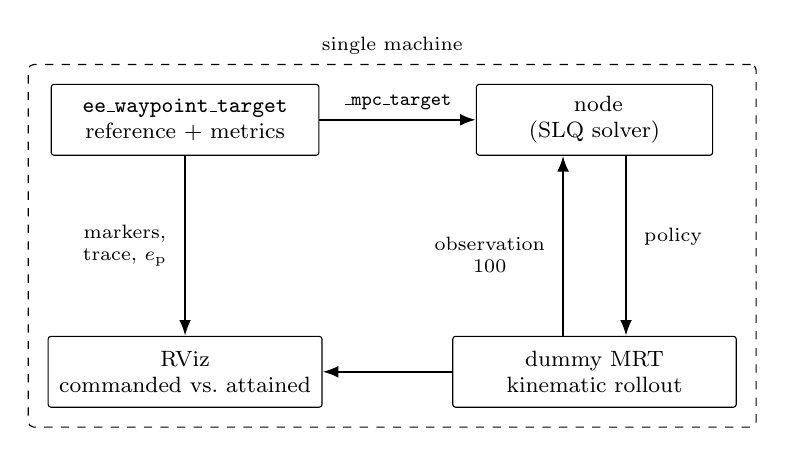
\begin{tikzpicture}[
      font=\footnotesize,
      box/.style={draw, rounded corners=1pt, align=center,
                  inner sep=4pt, minimum height=9mm},
      machine/.style={draw, dashed, rounded corners=2pt, inner sep=7pt},
      flow/.style={-{Latex[length=2mm]}, thick},
      lbl/.style={font=\scriptsize, align=center},
    ]
    \node[box, minimum width=34mm] (wp) at (0,0)
      {\texttt{ee\_waypoint\_target}\\reference + metrics};
    \node[box, minimum width=30mm] (mpc) at (5.2,0)
      {\mpc{} node\\(SLQ solver)};
    \node[box, minimum width=36mm] (dummy) at (5.2,-3.2)
      {dummy MRT\\kinematic rollout};
    \node[box, minimum width=28mm] (rviz) at (0,-3.2)
      {RViz\\commanded vs.\ attained};
    \node[machine, fit=(wp)(mpc)(dummy)(rviz),
          label={[lbl]above:single machine}] {};
    \draw[flow] (wp) -- (mpc)
      node[lbl, midway, above] {\texttt{\_mpc\_target}};
    \draw[flow] ([xshift=-4mm]dummy.north) -- ([xshift=-4mm]mpc.south)
      node[lbl, pos=0.45, left=1mm] {observation\\\qty{100}{\hz}};
    \draw[flow] ([xshift=4mm]mpc.south) -- ([xshift=4mm]dummy.north)
      node[lbl, pos=0.45, right=1mm] {policy};
    \draw[flow] (dummy.west) -- (rviz.east);
    \draw[flow] (wp.south) -- (rviz.north)
      node[lbl, midway, left=1mm] {markers,\\trace, $e_{\mathrm{p}}$};
  \end{tikzpicture}
  \caption[Dummy-MRT closed loop for Experiment~A]{%
    Dummy-MRT closed loop used to accept the Experiment~A configuration.
    The hardware bridge of \cref{fig:architecture} is replaced by a
    kinematic rollout of the latest policy; the waypoint node is
    otherwise unchanged.}
  \label{fig:sim-dummy-stack}
\end{figure}

\subsection{Commanded path}
\label{sec:sim-path}

The commanded path is an eight-corner rectangular parallelepiped whose
edges are aligned with the world axes after the box is landed
(\cref{fig:sim-box,tab:sim-waypoints}). ISO~9283 cl.~6.8.1 replaces a
cube by a parallelepiped when the travel along one axis is much smaller
than along the others~\cite{ISO9283}; here $z$ is an arm coordinate and
$x$, $y$ can recruit the base. The implemented box is smaller than the
workspace-filling $2.0\,\mathrm{m}\times 2.0\,\mathrm{m}\times
0.40\,\mathrm{m}$ parallelepiped discussed as a design target. Its
horizontal extents are \qty{0.60}{\meter} by \qty{0.80}{\meter} and its
height is \qty{0.25}{\meter}, with the lower face at
\qty{1.30}{\meter} and the upper face at \qty{1.55}{\meter}. The
perimeter is \qty{4.50}{\meter}.

Horizontal offsets are stored relative to the \ee{} pose at trigger
time (\texttt{origin\_frame: ee}); the $z$ values are absolute world
heights. Anchoring on the current \texttt{tool0} keeps the first corner
next to the standby pose, so the approach gate is a short motion rather
than a reach across the cell; the first offset is only
\qty{0.41}{\meter}. The far corner lies \qty{1.35}{\meter} from
that same \ee{}, which is enough to pull the base on the long edges
without demanding a $2\,\mathrm{m}$ translation on every lap. The
standby joint vector written in \texttt{task\_experiment\_a.info} (dummy
only; the hardware bridge ignores it) is the MoveIt named state
\texttt{bent}: shoulder pan, lift, elbow and wrist~1 at \ang{-90},
wrist~2 at \ang{+90}, wrist~3 at zero.

The visit order is a Hamiltonian cycle on the eight corners in which
every consecutive pair differs in a single coordinate:
\begin{equation*}
  \mathrm{P1}
    \xrightarrow{x}\mathrm{P2}
    \xrightarrow{y}\mathrm{P3}
    \xrightarrow{x}\mathrm{P4}
    \xrightarrow{z}\mathrm{P5}
    \xrightarrow{x}\mathrm{P6}
    \xrightarrow{y}\mathrm{P7}
    \xrightarrow{x}\mathrm{P8}
    \xrightarrow{z}\mathrm{P1}.
\end{equation*}
Six edges are horizontal and two are vertical. The vertical pair is a
pure arm motion in $z$; the base cannot contribute to it. Closing the
loop on a downward $z$ edge has a consequence for the ISO lead-out,
taken up below.

All eight knots share one orientation,
$\mathrm{RPY}=(\pi,\,0,\,-\pi/2)$, which is the \texttt{tool0} pose of
\texttt{bent} given the \ang{-90} mount of the arm
(\cref{sec:hero-platform}). A constant quaternion is required because
\texttt{TargetTrajectories::getDesiredState} interpolates quaternion
coefficients component-wise, not by spherical interpolation. A time-varying
reference orientation would inject interpolation error into
$e_{\mathrm{o}}$ that is not the controller's.

\begin{figure}[htbp]
  \centering
  \begin{tikzpicture}[
      font=\footnotesize,
      >=Latex,
      boxedge/.style={thick},
      zedge/.style={thick, dashed},
      lead/.style={thick, RWTHOrange100},
      pnt/.style={circle, fill=RWTHBlau100, inner sep=1.2pt},
      lbl/.style={font=\scriptsize},
    ]
    % scale: 1 m = 4.2 cm; x right = robot forward, y up = robot left
    \def\s{4.2}
    % bottom face z = 1.30
    \coordinate (P1) at ({0.40*\s}, {-0.10*\s});
    \coordinate (P2) at ({1.00*\s}, {-0.10*\s});
    \coordinate (P3) at ({1.00*\s}, {-0.90*\s});
    \coordinate (P4) at ({0.40*\s}, {-0.90*\s});
    % top face, offset to suggest height
    \coordinate (off) at (0.55, 0.70);
    \coordinate (P8) at ($(P1)+(off)$);
    \coordinate (P7) at ($(P2)+(off)$);
    \coordinate (P6) at ($(P3)+(off)$);
    \coordinate (P5) at ($(P4)+(off)$);
    \coordinate (Lin) at ({0.25*\s}, {-0.10*\s});
    % top rectangle (dashed) then bottom (solid), then verticals
    \draw[boxedge, dashed] (P8) -- (P7) -- (P6) -- (P5) -- cycle;
    \draw[boxedge] (P1) -- (P2) -- (P3) -- (P4) -- cycle;
    \draw[zedge] (P1) -- (P8);
    \draw[zedge] (P2) -- (P7);
    \draw[zedge] (P3) -- (P6);
    \draw[zedge] (P4) -- (P5);
    % measured Hamiltonian: P1-P2-P3-P4-P5-P6-P7-P8-P1
    \draw[->, very thick, RWTHBlau100] (P1) -- (P2);
    \draw[->, very thick, RWTHBlau100] (P2) -- (P3);
    \draw[->, very thick, RWTHBlau100] (P3) -- (P4);
    \draw[->, very thick, RWTHBlau100] (P4) -- (P5);
    \draw[->, very thick, RWTHBlau100] (P5) -- (P6);
    \draw[->, very thick, RWTHBlau100] (P6) -- (P7);
    \draw[->, very thick, RWTHBlau100] (P7) -- (P8);
    \draw[->, very thick, RWTHBlau100] (P8) -- (P1);
    \draw[lead, ->] (Lin) -- (P1);
    \foreach \p/\n/\a in {
      P1/P1/above, P2/P2/above, P3/P3/below,
      P4/P4/below, P5/P5/left, P6/P6/right,
      P7/P7/right, P8/P8/left} {
      \node[pnt] at (\p) {};
      \node[lbl, \a] at (\p) {\n};
    }
    \node[pnt, fill=RWTHOrange100] at (Lin) {};
    \node[lbl, above left] at (Lin) {lead-in};
    \node[lbl, anchor=west] at (5.0, -3.6)
      {solid: $z=\qty{1.30}{\meter}$; dashed: $z=\qty{1.55}{\meter}$};
    \node[lbl, anchor=west] at (5.0, -4.05)
      {$x$ forward (right), $y$ left (up)};
  \end{tikzpicture}
  \caption[Eight-corner commanded path for Experiment~A]{%
    Commanded parallelepiped in the \ee{}-anchored frame of
    \texttt{experiment\_a\_waypoints.yaml}. Blue arrows are the
    measured Hamiltonian cycle (segment identifiers $1$--$8$). The
    orange stub is the ISO~8.2 lead-in; the lead-out continues
    \qty{0.15}{\meter} down from P1 along the closing $z$ edge and is
    omitted here.}
  \label{fig:sim-box}
\end{figure}

\begin{table}[htbp]
  \centering
  \caption[Waypoint offsets of the Experiment~A box]{%
    Waypoint offsets of the Experiment~A box, copied from
    \texttt{experiment\_a\_waypoints.yaml}. $\Delta x$, $\Delta y$ are
    applied in the base yaw at trigger time about the current \ee{};
    $z$ is an absolute world height.}
  \label{tab:sim-waypoints}
  \begin{tabularx}{\linewidth}{@{}lXXXX@{}}
    \toprule
    Corner & $\Delta x$ / \si{\meter} & $\Delta y$ / \si{\meter}
      & $z$ / \si{\meter} & To next \\
    \midrule
    P1 & 0.40 & $-0.10$ & 1.30 & $+x$, \qty{0.60}{\meter} \\
    P2 & 1.00 & $-0.10$ & 1.30 & $-y$, \qty{0.80}{\meter} \\
    P3 & 1.00 & $-0.90$ & 1.30 & $-x$, \qty{0.60}{\meter} \\
    P4 & 0.40 & $-0.90$ & 1.30 & $+z$, \qty{0.25}{\meter} \\
    P5 & 0.40 & $-0.90$ & 1.55 & $+x$, \qty{0.60}{\meter} \\
    P6 & 1.00 & $-0.90$ & 1.55 & $+y$, \qty{0.80}{\meter} \\
    P7 & 1.00 & $-0.10$ & 1.55 & $-x$, \qty{0.60}{\meter} \\
    P8 & 0.40 & $-0.10$ & 1.55 & $-z$, \qty{0.25}{\meter} \\
    \bottomrule
  \end{tabularx}
\end{table}

\subsection{Time axis, state machine, and ISO legs}
\label{sec:sim-node}

Knot times are built on the \ocs{} relative axis
\texttt{observation.time}, never on the wall clock. A knot stamped in
wall time falls outside the receding horizon and the robot either freezes
or jumps to the last sample; that failure is cheap to see on the dummy
and expensive on hardware. At a trigger time $t_{0}$ the node walks the
landed corners, adding $\lVert \Delta\symbf{p}\rVert / v_{\mathrm{ref}}$
on every edge. The configured path speed is
$v_{\mathrm{ref}} = \qty{0.05}{\meter\per\second}$, half of the
\qty{0.10}{\meter\per\second} base limit in
\texttt{task\_experiment\_a.info}, so a dummy that cannot keep up is a
cost or constraint problem rather than a saturated plant. With
\texttt{corner\_dwell\_sec} $= \qty{2.0}{\second}$ the reference pauses
at each corner; the \qty{4.50}{\meter} perimeter then takes
\qty{90}{\second} of motion, and the seven dwells inside the measured
lap add \qty{14}{\second}, before lead-in and lead-out. A dwell of zero would
be the ISO path-accuracy mode (constant speed through corners). The
value used here is a pose-accuracy setting: the \ee{} is given time to
settle so that a later $\mathrm{AP}_{p}$ is not dominated by a corner
cut.

After \texttt{/start} the node does not immediately run the cycle. It
lands the box once, holds the reference at the lead-in point, and waits
until the measured \ee{} stays within
\qty{0.02}{\meter} of that point for \qty{0.3}{\second}
(\texttt{Approaching}). Only then does the running trajectory begin, so
the first measured edge does not contain the motion from standby. The
phase sequence is $\mathrm{Init}\to\mathrm{Hold}\to
\mathrm{Approaching}\to\mathrm{Running}\to\mathrm{Finished}$.
\texttt{auto\_start} is false: the box is drawn in RViz first, and a
service call starts the motion after a visual check.

ISO~9283 cl.~8.2 requires the programmed start and end to lie outside
the test path. A lead-in of \qty{0.15}{\meter} is placed on the backward
extension of P1--P2, and a lead-out of \qty{0.15}{\meter} on the tangent
of the closing edge. With the present Hamiltonian order that closing
edge is the downward $z$ leg, so the lead-out ends at
$z=\qty{1.15}{\meter}$. The dummy RViz configuration draws those legs
in orange for exactly this reason: a lead-out that would enter the
chassis is visible before anyone calls start. Returning to the standby
pose after the lead-out is switched off for this path
(\texttt{return\_to\_home: false}).

The trajectory is re-published at \qty{1}{\hz}. Re-sending the same
knots on the \ocs{} time axis is idempotent, but it restores the
reference if a reset handshake of the MRT bridge has overwritten it
with a two-sample hold (\cref{sec:hw-interfaces}). The dummy rarely
handshakes again in mid-run; the timer is still part of the node that
hardware will use.

Relative to \texttt{task\_hardware.info} (\cref{tab:mpc-config}), the
experiment file lowers the pre-scale diagonal of $R_{\mathrm{base}}$
from $8.5$ to $5.5$, replaces the uniform arm diagonal of $4.0$ by
per-joint values between $2.5$ and $4.0$, and raises the \ee{} position
weight from $10$ to $\mu_{\mathrm{p}}=16$ while lowering the orientation
weight from $5$ to $\mu_{\mathrm{o}}=3$. A cheaper base and a tighter
position term are what push the solver to reach the far corners by
driving the platform instead of stretching the arm towards its reach
limit. The file also lengthens the horizon from \qty{1.2}{\second} to
$T=\qty{1.3}{\second}$ and the solution time window from
\qty{1.0}{\second} to $T_{\mathrm{sol}}=\qty{1.2}{\second}$; solve and
evaluation rates stay at \qty{10}{\hz} and \qty{100}{\hz}. The dummy
therefore validates that operating point, not the everyday hardware
tune.

\subsection{Procedure and acceptance}
\label{sec:sim-acceptance}

A dummy session is started with
\texttt{experiment\_a\_dummy.launch.py}. After the first observation the
box appears in RViz, including the orange lead legs. The operator
confirms that every corner is in the cell and that the lead-out at
$z=\qty{1.15}{\meter}$ clears the chassis, then calls
\texttt{/ee\_waypoint\_target/start}. The dummy plant must reach the
entry point, traverse all eight measured edges, and finish on the
lead-out hold without the reference jumping to the last knot. The
metric topic must show \texttt{segment\_id} passing through $1$--$8$
and returning to a negative identifier. Those checks accept the
geometry, the \ocs{} time axis, the data pipeline and the visualisation.
They do not produce a tracking-accuracy number for the robot.

The same YAML and task file are the input of the mock-hardware and
physical runs in \cref{ch:hardware}. A planar four-corner variant
exists as a reduced path at constant $z$ and shares this node; it is
not used in the dummy checks reported here.

What the dummy cannot close is the list in
\cref{sec:sim-methodology}: policy lag, actuator dynamics, odometry
drift, and any ISO claim that needs an external \ee{} pose, $n\ge 3$
cycles, or a second pipeline. Those belong to the hardware chapter,
using the metrics of \cref{tab:sim-metrics} on the measured segments of
the path in \cref{fig:sim-box}.

% !TeX root = ../main.tex
\chapter{Hardware Deployment and Preliminary Experimental Results}
\label{ch:hardware}

The dummy loop of \cref{ch:simulation} accepts the Experiment~A files on
a kinematic plant. This chapter takes the same files through the MRT
bridge of \cref{sec:hw-interfaces}: first with mock
\texttt{ros2\_control} interfaces that echo commands into state, then on
the physical \hero{} platform. The mock still has policy lag, velocity
clamps and the Zenoh boundary; what it does not have is actuator
dynamics or wheel-odometry drift. The gap between the two sessions is
therefore the contribution of the plant and of the state estimate, on
top of a residual that the dummy never sees.

\Cref{sec:hw-deployment} records how the deployment was started
and which sessions are reported. \Cref{sec:hw-challenges} treats the
timing and model problems that show up once the bridge is in the loop.
\Cref{sec:hw-results} compares one mock lap with one hardware lap on the
eight-corner path of \cref{fig:sim-box}, using the metrics of
\cref{tab:sim-metrics}. Both traces are internal metrology
(\cref{sec:sim-metrology}). A single slow lap is not an ISO~9283
test~\cite{ISO9283}, and it is not yet a comparison with a decoupled
baseline.

% ---------------------------------------------------------------------
\section{Deployment on the \hero{} Platform}
\label{sec:hw-deployment}

The topology is that of \cref{sec:distributed-arch}: the
external PC solves the optimal-control problem and publishes the
Experiment~A reference; the on-board IPC evaluates the policy and
commands the drives. Both machines run the project containers on
ROS~2~Jazzy with the Zenoh middleware. The external PC was attached to
the platform subnet by Ethernet for every session below. The wireless
access point of the platform remains a possible join path, and was the
reason Zenoh was chosen in the first place, but it was not used as the
control link here: a cable avoids the jitter that made DDS unusable on
that hop, at the price of tethering a \qty{400}{\kilo\gram} base to a
desk. The box of \cref{fig:sim-box} is small enough that the cable did
not go taut in the recorded laps; it is still a run condition, not a
property of the controller.

Start-up follows the order already required by the reset handshake.
Each machine starts its Zenoh router, the external PC router pointing at
the IPC. The Experiment~A host launch then brings up the \mpc{} node, the
waypoint target node and RViz, with the same task file and waypoint file
the dummy used. Only after the reset service is advertised is the IPC
launch started, so that the bridge can handshake immediately rather than
wait. On the first start after a model change the external PC still
spends about a minute compiling CppAD libraries; later starts reuse the
cache. RViz is checked before anyone calls \texttt{/start}: the landed
box, the orange lead legs, and in particular the lead-out at
$z=\qty{1.15}{\meter}$, have to sit in free space. The approaching gate
of \cref{sec:sim-node} then holds the reference at the lead-in until the
measured \ee{} is within \qty{0.02}{\meter} of that point. Orientation
is not part of the gate, so a residual attitude at entry is admitted
into the first measured edge.

A mock session is the same pair of launches with
\texttt{mock\_arm:=true} and \texttt{mock\_platform:=true} on the IPC
side. The controller manager, the MRT bridge and the three \ocs{}
streams across Zenoh are those of the hardware stack; only the
\texttt{ros2\_control} hardware interfaces are replaced by echo
components~\cite{ros2control}. That is a stricter check than the dummy,
and a weaker one than the robot. It is the last run that can still be
repeated at a desk.

Closed-loop motion on the physical platform was obtained before the
sessions reported here. Those earlier laps are omitted, because the
approaching gate, the segment identifiers and the metric topic were not
yet the pipeline of \cref{ch:simulation}. The traces below are one mock
lap and one hardware lap recorded on 14~August~2026, at the operating
point of \cref{sec:sim-node}: path speed
$\qty{0.05}{\meter\per\second}$, corner dwell $\qty{2.0}{\second}$,
horizon $T=\qty{1.3}{\second}$, solution time window
$T_{\mathrm{sol}}=\qty{1.2}{\second}$, feed-forward SLQ with one
iteration, $\mu_{\mathrm{p}}=16$, $\mu_{\mathrm{o}}=3$, and
$R_{\mathrm{base}}$ pre-scale $5.5$. The solver on the external PC used
eight threads. Host and IPC logs were kept alongside the bags
(\texttt{bag\_host\_0814\_1558} mock,
\texttt{bag\_host\_0814\_1613} hardware). Metrics are computed from the
exported \texttt{ee\_metrics} and solver-diagnostics streams, restricted
to $\texttt{segment\_id}\ge 1$ as in \cref{sec:sim-pose-error}.

% ---------------------------------------------------------------------
\section{Deployment Challenges and Mitigations}
\label{sec:hw-challenges}

The real-time invariant of \cref{eq:rt-invariant} was written for the
everyday file \texttt{task\_hardware.info}, where
$T_{\mathrm{sol}}=\qty{1.0}{\second}$. The Experiment~A file widens that
window to $\qty{1.2}{\second}$ so that a slow solve can still hand the
bridge a policy before the
previous one expires. On the hardware lap the last-solve time had mean
$\qty{227}{\milli\second}$, median $\qty{218}{\milli\second}$ and 95th
percentile $\qty{297}{\milli\second}$; the slowest sample in that stream
was $\qty{353}{\milli\second}$, and the solver's own running maximum
reached $\qty{720}{\milli\second}$. Policies arrived at
$\qty{4.4}{\hz}$. Twice the mean solve, $\qty{0.45}{\second}$, is still
less than $T_{\mathrm{sol}}$, and the bridge did not enter a
policy-exhaustion hold on this lap. The loop therefore ran in real time
in the sense of \cref{eq:rt-invariant}, although policies arrived at
less than half the $\qty{10}{\hz}$ named by \texttt{mpcDesiredFrequency};
on the robot that entry throttles nothing (\cref{sec:hw-interfaces}).

The mock lap was faster on average (mean $\qty{174}{\milli\second}$,
effective $\qty{5.8}{\hz}$) but not safer in the tail. One solve took
$\qty{1.12}{\second}$, which is inside the $\qty{1.2}{\second}$ window
and would have been past the $\qty{1.0}{\second}$ window of the everyday
file. The bridge logged three ``policy nearly exhausted'' warnings on
that lap; the hardware lap logged none. \ocs{} still printed its
``solution time window might be shorter than the MPC delay'' warning
once on the robot and nine times on the mock. The warning compares the
window with an internal delay estimate and is not the same test as a
hold. Widening $T_{\mathrm{sol}}$ is what kept the spike from freezing
the mock plant. It does not make a $\qty{10}{\hz}$ solver out of a
$\qty{4}{\hz}$ one. \Cref{fig:hw-solve-ecdf} puts the two distributions
side by side.

\begin{figure}[htbp]
  \centering
  \begin{tikzpicture}
    \begin{axis}[
        width=0.92\linewidth, height=6.0cm,
        xmode=log,
        log ticks with fixed point,
        xlabel={last-solve time / \si{\milli\second}},
        ylabel={fraction of solves at or below},
        xmin=100, xmax=1300,
        ymin=0, ymax=1.03,
        xtick={100,150,200,300,500,800,1200},
        ytick={0,0.25,0.5,0.75,0.95},
        yticklabels={$0$,$0.25$,$0.50$,$0.75$,$0.95$},
        x tick label style={/pgf/number format/1000 sep={}},
        legend pos=north west,
      ]
      \addplot[RWTHBlau100, thick, const plot, no marks]
        table[x=ms, y=frac] {03_figures/hw_mock_solve_ecdf.dat};
      \addplot[RWTHOrange100, thick, const plot, no marks]
        table[x=ms, y=frac] {03_figures/hw_real_solve_ecdf.dat};
      \addplot[gray, dotted, forget plot, domain=100:1300, samples=2] {0.95};
      \addplot[black, dashed, forget plot] coordinates {(1000,0) (1000,1.03)};
      \addplot[black, densely dashdotted, forget plot]
        coordinates {(1200,0) (1200,1.03)};
      \legend{mock, robot}
      \node[anchor=east, font=\scriptsize] at (axis cs:980,0.58)
        {\qty{1.0}{\second}};
      \node[anchor=east, font=\scriptsize] at (axis cs:1180,0.40)
        {\qty{1.2}{\second}};
    \end{axis}
  \end{tikzpicture}
  \caption[Distribution of last-solve time on the mock and hardware
    sessions]{%
    Empirical distribution of the last-solve time on the two laps, on a
    logarithmic axis; \cref{fig:hw-solve} shows the same two streams
    against wall time. The mock curve sits to the left of the robot curve
    over most of its range---the mock solves faster at the median,
    \qty{163}{\milli\second} against \qty{218}{\milli\second}---but it is
    the mock that carries the tail: its slowest solve is
    \qty{1.12}{\second}, against \qty{353}{\milli\second} on the robot,
    and about one mock solve in a hundred exceeds \qty{400}{\milli\second}
    where the robot stream ends. The dashed line is the solution time
    window of \texttt{task\_hardware.info} and the dash-dotted line the
    wider window of the Experiment~A file; the mock spike falls between
    them, which is why it expired a policy under the everyday setting but
    not under the one actually used (\cref{eq:rt-invariant}).}
  \label{fig:hw-solve-ecdf}
\end{figure}

Because a new policy is already old when it arrives, the input that the
bridge applies is never the one at $\tau=0$ of the horizon.
\Cref{fig:hw-lag} sketches the timing. On the hardware lap the lag at
policy arrival---solve time plus the Zenoh hop---had mean
$\qty{0.24}{\second}$ and 95th percentile $\qty{0.32}{\second}$ after
the first few samples, against a maximum of $\qty{0.36}{\second}$.
Between arrivals the bridge keeps evaluating the same policy, so the lag
at the interpolation site grows until the next message; that quantity
had mean $\qty{0.36}{\second}$. The mock figures were
$\qty{0.18}{\second}$ at arrival and $\qty{0.29}{\second}$ at
interpolation. In both cases the first one to two tenths of a second of
every plan are unused. Diagnostics
\texttt{[policy\_arrival]} and \texttt{[policy\_interp]} were left
enabled at $\qty{0.1}{\second}$ on the IPC launch so that these numbers
could be read from the log rather than inferred from solve time alone.

\begin{figure}[htbp]
  \centering
  \begin{tikzpicture}[
      font=\footnotesize,
      >=Latex,
      lbl/.style={font=\scriptsize, align=center},
    ]
    \draw[->] (0,0) -- (12.2,0) node[right] {$\tau$};
    \foreach \x/\t in {0/0, 2.2/0.24, 3.3/0.36, 11.0/1.3} {
      \draw (\x, 0.12) -- (\x, -0.12);
      \node[below, lbl] at (\x, -0.12) {$\t\,\mathrm{s}$};
    }
    \draw[very thick, RWTHBlau100] (0, 0.85) -- (11.0, 0.85);
    \node[lbl, anchor=west] at (0, 1.25)
      {policy valid on $[t_0,\,t_0+T]$, $T=\qty{1.3}{\second}$};
    \fill[RWTHOrange100] (0, 0.85) circle (2.2pt);
    \node[lbl, above] at (0, 0.95) {$t_0$ snapshot};
    \draw[RWTHOrange100, thick] (0, 0.55) -- (2.2, 0.55);
    \node[lbl, above] at (1.1, 0.55) {solve $+\mathrm{net}$};
    \fill[RWTHBlau100] (2.2, 0.85) circle (2.2pt);
    \node[lbl, above] at (2.2, 0.95) {arrival};
    \draw[thick, dashed, RWTHOrange100] (2.2, 0.85) -- (3.3, 0.85);
    \fill[black] (3.3, 0.85) circle (2.2pt);
    \node[lbl, above] at (3.6, 1.15) {typical evaluation};
    \draw[<->] (0, -0.85) -- (2.2, -0.85);
    \node[lbl, below] at (1.1, -0.85)
      {unused prefix $\approx\qty{0.24}{\second}$};
  \end{tikzpicture}
  \caption[Policy lag on the hardware lap]{%
    Policy lag on the hardware lap. A plan stamped at the snapshot
    $t_0$ becomes available only after the solve and the network hop,
    and is then read at a time that continues to advance until the next
    plan arrives. Times are the measured means of that session, not
    configuration values.}
  \label{fig:hw-lag}
\end{figure}

If that prefix contains the only aggressive correction the solver is
willing to apply, the robot never receives it. The \ocs{} model is a
kinematic integrator: a large velocity at $\tau=0$ really would cancel a
position error in a few tens of milliseconds, and a high
$\mu_{\mathrm{p}}$ encourages exactly that pulse. The recorded policy
topic stores the first input of each plan, not the input at the
interpolation time, so this chapter cannot show the pulse being skipped
on these laps. What it can show is a consistency check. Along-track lag
$t_{\mathrm{lag}}$ of \cref{eq:lag-eff} should be comparable to the
interpolation lag if delay is the whole story. On the mock it is
(mean $t_{\mathrm{lag}}=\qty{0.39}{\second}$ against
$\qty{0.29}{\second}$ of interpolation lag). On the robot it is not
(mean $t_{\mathrm{lag}}=\qty{1.81}{\second}$). Delay explains the mock
residual and does not explain the hardware residual.

Two other failure modes of the bridge were already designed around and
barely appeared in these sessions. A mid-run reset handshake still
replaces the reference with a two-knot hold at the current \ee{}; the
waypoint node re-publishes the same knots at $\qty{1}{\hz}$ on the
\ocs{} time axis so that a lost reference comes back without a step in
the command. The arm rate clamp of \cref{tab:bridge-guards} issued two
warnings on each lap, which is not a dominant trace. Protective stops
and teach-pendant mode errors, which dominated the first bring-up of the
IPC launch, are operational rather than closed-loop problems: the UR
driver has to start in headless remote mode, and the controller stopper
has to keep the joint-trajectory controller in its ignore list, as
already required in \cref{sec:hw-interfaces}. They are mentioned here
only because a session that skips those checks never produces a bag.

The remaining limitation is the model. Mock hardware realises the
integrator: commanded wheel and joint rates appear in the next
observation. The physical base is a \qty{400}{\kilo\gram} platform whose
drive controller enforces its own acceleration
limit~\cite{HenkelRoth2019freeMoVe}, and the UR10e in streaming position
control has a following error that the kinematic model does not
know~\cite{UR10e}. Every re-solve on the robot therefore starts from a
state the previous plan did not expect. That is a different problem from
a slow solver, and \cref{sec:hw-results} is mostly about it.

% ---------------------------------------------------------------------
\section{Preliminary End-Effector Tracking Results}
\label{sec:hw-results}

Both sessions completed the eight measured edges and finished on the
lead-out hold at $z=\qty{1.15}{\meter}$. The mock approaching gate ran
for $\qty{10}{\second}$ from an initial \ee{} error of
$\qty{1.04}{\meter}$; the robot needed $\qty{19}{\second}$ from
$\qty{0.34}{\meter}$, longer than the mock from a third of the
distance, and entered \texttt{RUNNING} at
$\qty{19}{\milli\meter}$ with an orientation error of
$\qty{0.061}{\radian}$ that the gate does not wait for. From the first
sample with $\texttt{segment\_id}\ge 1$ to the last, both laps lasted
$\qty{104}{\second}$, which is the commanded
$\qty{4.50}{\meter}/\qty{0.05}{\meter\per\second}$ plus seven corner
dwells of $\qty{2}{\second}$ (the last corner has no dwell before the
lead-out). Task-completion time $T$ of \cref{tab:sim-metrics} therefore
does not distinguish the two plants. Path shape does.

\Cref{fig:hw-path} shows the commanded and attained \ee{} paths in a
frame attached to the first corner, with $x$ along P1--P2 and $y$ along
the leftward horizontal edge. The vertical edges of the box collapse in
this view; they remain in the error signals. On the mock the attained
path follows the rectangle with a lag that is visible mainly as a
short-cut at the corners. On the robot the attained path is a rounded,
inward-offset copy of the same rectangle, with a consistent bias of
order \qty{10}{\centi\meter} rather than a delay that stays on the
line.

\begin{figure}[htbp]
  \centering
  \begin{subfigure}[t]{0.48\textwidth}
    \centering
    \begin{tikzpicture}
      \begin{axis}[
          width=0.95\linewidth, height=6.1cm,
          xlabel={$x$ / \si{\meter}},
          ylabel={$y$ / \si{\meter}},
          xmin=-0.12, xmax=0.78, ymin=-0.12, ymax=0.95,
          axis equal image,
          legend pos=north west,
        ]
        \addplot[black, thick] table {03_figures/hw_mock_des.dat};
        \addplot[RWTHBlau100, thick] table {03_figures/hw_mock_act.dat};
        \legend{commanded, attained}
      \end{axis}
    \end{tikzpicture}
    \caption{Mock hardware}
    \label{fig:hw-path-mock}
  \end{subfigure}
  \hfill
  \begin{subfigure}[t]{0.48\textwidth}
    \centering
    \begin{tikzpicture}
      \begin{axis}[
          width=0.95\linewidth, height=6.1cm,
          xlabel={$x$ / \si{\meter}},
          ylabel={$y$ / \si{\meter}},
          xmin=-0.12, xmax=0.78, ymin=-0.12, ymax=0.95,
          axis equal image,
          legend pos=north west,
        ]
        \addplot[black, thick] table {03_figures/hw_real_des.dat};
        \addplot[RWTHOrange100, thick] table {03_figures/hw_real_act.dat};
        \legend{commanded, attained}
      \end{axis}
    \end{tikzpicture}
    \caption{Physical robot}
    \label{fig:hw-path-real}
  \end{subfigure}
  \caption[Commanded and attained \ee{} paths, mock versus hardware]{%
    Commanded and attained \ee{} paths on the measured edges, in a
    frame with origin at P1 and $x$ along P1--P2. The two vertical
    edges of \cref{fig:sim-box} project onto the short sides.}
  \label{fig:hw-path}
\end{figure}

\Cref{tab:hw-metrics} collects the scalar scores. Time-aligned position
error $e_{\mathrm{p}}$ on the mock had RMS \qty{27}{\milli\meter} and
maximum \qty{71}{\milli\meter}; on the robot the same quantities were
\qty{130}{\milli\meter} and \qty{204}{\milli\meter}. Mean Hausdorff
$\overline{H}$ rose from \qty{12}{\milli\meter} to
\qty{62}{\milli\meter}, and the 95th percentile of the nearest-neighbour
distances from \qty{23}{\milli\meter} to \qty{110}{\milli\meter}. The
classical $H$ is dominated by a single mock sample at
\qty{71}{\milli\meter} and is the weaker summary, which is why
\cref{sec:sim-path-metrics} asked for $\overline{H}$ and $P_{95}$ as
well. Orientation error grew with the plant too: RMS
\qty{0.056}{\radian} on the mock, \qty{0.27}{\radian} on the robot, with
a hardware maximum of \qty{0.47}{\radian} on later edges. With
$n=1$ cycle, ISO path accuracy $\mathrm{AT}_{p}$ is not reported as a
standard value; $h(B,A)$ on the densely resampled command is the nearest
stand-in and sits at \qty{71}{\milli\meter} (mock) and
\qty{123}{\milli\meter} (robot).

\begin{table}[htbp]
  \centering
  \caption[Mock versus hardware scores on the measured Experiment~A lap]{%
    Mock versus hardware scores on the measured Experiment~A lap
    ($\texttt{segment\_id}\ge 1$). Hausdorff quantities use a
    \qty{1}{\milli\meter} resampling of the commanded polyline, as in
    \cref{sec:sim-path-metrics}. Solve time is the last-solve sample of
    the diagnostics stream; policy lag at arrival is the MRT
    \texttt{policyLagAtArrival} log, excluding the first five samples.}
  \label{tab:hw-metrics}
  \begin{tabularx}{\linewidth}{@{}lXX@{}}
    \toprule
      & Mock hardware & Physical robot \\
    \midrule
    $e_{\mathrm{p}}$ RMS (max)
      & \qty{27}{\milli\meter} (\qty{71}{\milli\meter})
      & \qty{130}{\milli\meter} (\qty{204}{\milli\meter}) \\
    $e_{\mathrm{o}}$ RMS (max)
      & \qty{0.056}{\radian} (\qty{0.13}{\radian})
      & \qty{0.27}{\radian} (\qty{0.47}{\radian}) \\
    $H$ / $\overline{H}$ / $P_{95}$
      & \qty{71}{\milli\meter} / \qty{12}{\milli\meter} /
        \qty{23}{\milli\meter}
      & \qty{135}{\milli\meter} / \qty{62}{\milli\meter} /
        \qty{110}{\milli\meter} \\
    mean $t_{\mathrm{lag}}$
      & \qty{0.39}{\second}
      & \qty{1.81}{\second} \\
    mean solve time (effective rate)
      & \qty{174}{\milli\second} (\qty{5.8}{\hz})
      & \qty{227}{\milli\second} (\qty{4.4}{\hz}) \\
    mean policy lag at arrival
      & \qty{0.18}{\second}
      & \qty{0.24}{\second} \\
    measured lap $T$
      & \qty{104}{\second}
      & \qty{104}{\second} \\
    \bottomrule
  \end{tabularx}
\end{table}

\Cref{fig:hw-error} plots $e_{\mathrm{p}}(t)$ on the measured edges,
with time zero at the first admitted sample. The mock trace stays below
\qty{50}{\milli\meter} except for a short spike at the first corner. The
hardware trace climbs through the first long edge, plateaus around
\qty{15}{\centi\meter} to \qty{20}{\centi\meter} on edges 2--4 and~6, and
only comes back toward \qty{5}{\centi\meter} on the last horizontal
edge. It is not a delayed copy of the mock.

\begin{figure}[htbp]
  \centering
  \begin{tikzpicture}
    \begin{axis}[
        width=0.92\linewidth, height=5.6cm,
        xlabel={time on measured path / \si{\second}},
        ylabel={$e_{\mathrm{p}}$ / \si{\milli\meter}},
        xmin=0, xmax=105, ymin=0, ymax=220,
        legend pos=north west,
      ]
      \addplot[RWTHBlau100, thick] table {03_figures/hw_mock_ep.dat};
      \addplot[RWTHOrange100, thick] table {03_figures/hw_real_ep.dat};
      \legend{mock, robot}
    \end{axis}
  \end{tikzpicture}
  \caption[Time-aligned \ee{} position error on the measured path]{%
    Time-aligned \ee{} position error on the measured path. Time zero is
    the first sample with $\texttt{segment\_id}\ge 1$.}
  \label{fig:hw-error}
\end{figure}

Per-edge numbers make the same split (\cref{tab:hw-segments}). The mock
RMS stays between \qty{10}{\milli\meter} and \qty{41}{\milli\meter} on
every edge. The robot is already at \qty{69}{\milli\meter} RMS on the
opening \qty{0.60}{\meter} edge and peaks at \qty{175}{\milli\meter} on
edge~3. The two vertical edges (4 and~8), which the base cannot help
with, are not the worst hardware edges; the long horizontal edges are.
Along-track error on the robot is positive on seven of the eight edges
and has mean \qty{91}{\milli\meter}, which at
$v_{\mathrm{ref}}=\qty{0.05}{\meter\per\second}$ is the
$\qty{1.81}{\second}$ of $t_{\mathrm{lag}}$ already quoted. A pure
policy-lag prediction $0.36\,\mathrm{s}\times v_{\mathrm{ref}}$ is only
\qty{18}{\milli\meter}. The mock along-track mean, \qty{19}{\milli\meter},
matches that prediction. The extra \qty{70}{\milli\meter} on the robot
is not delay in the MRT bridge.

\begin{table}[htbp]
  \centering
  \caption[Per-edge \ee{} position error on the measured lap]{%
    Per-edge \ee{} position error on the measured lap. Edges 1, 3, 5
    and~7 are the \qty{0.60}{\meter} sides; 2 and~6 are the
    \qty{0.80}{\meter} sides; 4 and~8 are the vertical \qty{0.25}{\meter}
    sides.}
  \label{tab:hw-segments}
  \begin{tabularx}{\linewidth}{@{}lXXXX@{}}
    \toprule
    Edge & Mock RMS & Mock max & Robot RMS & Robot max \\
    \midrule
    1 & \qty{16}{\milli\meter} & \qty{71}{\milli\meter}
      & \qty{69}{\milli\meter} & \qty{80}{\milli\meter} \\
    2 & \qty{41}{\milli\meter} & \qty{53}{\milli\meter}
      & \qty{143}{\milli\meter} & \qty{187}{\milli\meter} \\
    3 & \qty{10}{\milli\meter} & \qty{18}{\milli\meter}
      & \qty{175}{\milli\meter} & \qty{204}{\milli\meter} \\
    4 & \qty{31}{\milli\meter} & \qty{45}{\milli\meter}
      & \qty{145}{\milli\meter} & \qty{174}{\milli\meter} \\
    5 & \qty{22}{\milli\meter} & \qty{26}{\milli\meter}
      & \qty{98}{\milli\meter} & \qty{129}{\milli\meter} \\
    6 & \qty{30}{\milli\meter} & \qty{35}{\milli\meter}
      & \qty{169}{\milli\meter} & \qty{202}{\milli\meter} \\
    7 & \qty{18}{\milli\meter} & \qty{21}{\milli\meter}
      & \qty{60}{\milli\meter} & \qty{140}{\milli\meter} \\
    8 & \qty{39}{\milli\meter} & \qty{45}{\milli\meter}
      & \qty{111}{\milli\meter} & \qty{160}{\milli\meter} \\
    \bottomrule
  \end{tabularx}
\end{table}

Corner dwells isolate the same point without mixing it into a moving
reference. On the mock, the last $\qty{2}{\second}$ of edges 1--7---the
dwell windows---fall to between \qty{5}{\milli\meter} and
\qty{25}{\milli\meter}. On the robot the same windows remain between
\qty{53}{\milli\meter} and \qty{168}{\milli\meter} and do not collapse.
Once the command has stopped, a lag of $\qty{0.36}{\second}$ should
have died out. What remains is a steady offset that the receding-horizon
loop does not remove at this operating point.

Solve time over the two sessions is shown in \cref{fig:hw-solve} only to
close the timing discussion. After the first seconds both traces sit
near their means; the mock spike to $\qty{1.12}{\second}$ is the event
that produced the exhaustion warnings. Neither curve tracks
$e_{\mathrm{p}}(t)$. A slow solver would have frozen the robot through
the hold logic of \cref{tab:bridge-guards}. That did not happen. The
tracking gap is left by the plant and by the lag acting on a model that
assumes the plant is an integrator.

\begin{figure}[htbp]
  \centering
  \begin{tikzpicture}
    \begin{axis}[
        width=0.92\linewidth, height=5.2cm,
        xlabel={wall time from first diagnostic / \si{\second}},
        ylabel={last solve time / \si{\second}},
        xmin=0, xmax=210, ymin=0, ymax=1.25,
        legend pos=north east,
      ]
      \addplot[RWTHBlau100, thick] table {03_figures/hw_mock_solve.dat};
      \addplot[RWTHOrange100, thick] table {03_figures/hw_real_solve.dat};
      \addplot[black, dashed, domain=0:210] {0.1};
      \addplot[gray, dashed, domain=0:210] {1.2};
      \legend{mock, robot, $\qty{10}{\hz}$ period, $T_{\mathrm{sol}}$}
    \end{axis}
  \end{tikzpicture}
  \caption[Last-solve time on the mock and hardware sessions]{%
    Last-solve time on the mock and hardware sessions. The lower dashed
    line is the $\qty{0.1}{\second}$ period of \texttt{mpcDesiredFrequency},
    which the bridge uses only as its warning threshold; the upper line is
    $T_{\mathrm{sol}}=\qty{1.2}{\second}$.}
  \label{fig:hw-solve}
\end{figure}

Two caveats bound what these numbers may be used for. First, both
desired and attained poses are reconstructed from the \mpc{} observation,
so wheel-odometry drift is shared by the command frame and the measured
\ee{}. On the robot the box was landed at a base pose near
$(23.2,\,9.0)$ in the odometry frame, which is the accumulated motion of
the platform before this lap, not a localisation in the hall. Closed-loop
drift of the attained path relative to its own start was
\qty{15}{\centi\meter} on the robot and \qty{11}{\centi\meter} on the
mock, most of it in $z$ at the last vertical edge rather than a planar
loop-closure error. None of this is an ISO accuracy statement; an
external \ee{} pose is still missing. Second, each plant was run once, at
one speed, without a decoupled baseline. Repeatability $\mathrm{RT}_{p}$,
the three speed levels of ISO Table~3, and a Nav2 plus MoveIt comparison
are outside the present
data~\cite{ISO9283,Macenski2020Nav2,moveit2}.

What the pair of laps does show is narrower. The Experiment~A files that
the dummy accepted can be executed by the hardware stack from approaching
gate to lead-out hold. Mock hardware, which shares the bridge and the
lag with the robot, tracks at a few centimetres and at an along-track
delay consistent with policy lag. The physical platform, with the same
files, tracks at one to two decimetres and does not catch the reference
during dwell. The next improvements that would change those numbers are
a shorter solve (so that $u(\tau=0)$ is no longer in the past), a model
that knows the base cannot step in velocity, and an external pose of the
\texttt{tool0} frame.

% !TeX root = ../main.tex
\chapter{Conclusion and Outlook}
\label{ch:conclusion}

This chapter closes the thesis by returning to the objective of
\cref{sec:objectives}: integrate whole-body \mpc{} on the physical
\hero{} platform and characterise its \ee{}-tracking behaviour. The
preceding chapters have already separated what the optimiser does on its
kinematic model (\cref{ch:simulation}), what the MRT bridge adds
(\cref{sec:hw-challenges}), and what the plant adds on top
(\cref{sec:hw-results}). What follows is a concise account of what was
achieved, what the present data do and do not establish, and which
engineering steps would most directly change the numbers reported in
\cref{ch:hardware}.

% ---------------------------------------------------------------------
\section{Summary}
\label{sec:concl-summary}

The work set out to move \ocs{} whole-body \mpc{} from a framework
demonstration to a deployable stack on a differential-drive mobile
manipulator in an LMAS-oriented setting. Against that goal, four
contributions were delivered.

First, a whole-body motion-planning approach was selected for the
\hero{} platform after comparing \ocs{} with alternative frameworks
(\cref{ch:sota}). Second, \ocs{} was integrated into the existing
software stack: a split host/on-board deployment over Zenoh keeps the
actuation path local to the IPC while the SLQ solver runs on a
workstation (\cref{sec:distributed-arch}); a nine-state kinematic model
with non-holonomic base, safety-panel joint limits, and a reduced
self-collision set was parameterised for on-robot operation (\cref{sec:wholebody-model});
and an MRT bridge turns the published policy into wheel and joint
commands under explicit guards (\cref{sec:hw-interfaces}). Third, a
simulation-based acceptance path was built around Experiment~A: the same
task file and waypoint list that the robot will load are exercised in a
dummy MRT loop, with internal metrology and ISO-oriented path metrics
defined before any hardware session (\cref{ch:simulation}). Fourth, that
configuration was taken through mock \texttt{ros2\_control} hardware and
onto the physical platform. The closed eight-corner path of
\cref{fig:sim-box} completed on both plants; the approaching gate,
segment tagging, and lead-out hold that \cref{sec:sim-node} specifies all
appeared in the recorded sessions.

The tracking outcome is more qualified. On mock hardware, which shares
the bridge and the policy lag with the robot but replaces the plant by
command echoing, the attained \ee{} path followed the commanded rectangle
at a few centimetres (\cref{tab:hw-metrics}). On the physical robot, with
the same files and the same wall-clock lap duration, position error
remained at one to two decimetres on the long edges and did not collapse
during corner dwells (\cref{fig:hw-error,tab:hw-segments}). The loop
therefore ran in real time in the sense of \cref{eq:rt-invariant}---no
policy-exhaustion hold occurred on the hardware lap---but the effective
\mpc{} rate was about \qty{4.4}{\hz} against a \qty{10}{\hz} request, and
the first one to two tenths of a second of each plan were lost to solve
time and network delay before the bridge could apply them
(\cref{fig:hw-lag}). Along-track lag consistent with that delay explains
the mock residual; it does not explain the larger hardware offset
(\cref{sec:hw-challenges}).

Several constraints bound how strongly these results can be read. All
desired and attained poses were reconstructed from wheel odometry and
joint encoders inside the waypoint node (\cref{sec:sim-metrology}), so
the scores measure internal consistency of the closed loop, not absolute
accuracy in the hall. Each plant was exercised once, at
$v_{\mathrm{ref}}=\qty{0.05}{\meter\per\second}$, without the three
mandatory ISO speed levels or repeated cycles. The workstation was
connected by Ethernet throughout (\cref{sec:hw-deployment}); the numbers
therefore do not speak to control over the platform's wireless link. The
\ocs{} model treats the base as a velocity integrator and knows nothing
of the drive controller's acceleration limit or of the UR10e following
error under streaming position control. Finally, no decoupled Nav2 plus
MoveIt baseline was run on the same path, so the thesis validates
whole-body execution and characterises its residual; it does not yet
demonstrate superiority over sequential planning on identical metrics.

% ---------------------------------------------------------------------
\section{Critical Reflection}
\label{sec:concl-reflection}

The experiments answer a narrower question than the LMAS motivation of
\cref{sec:lmas} might suggest. They show that a time-parameterised
\ee{} reference, published as \ocs{} \texttt{TargetTrajectories} rather
than as a sequence of static goals, can be executed end to end on
\hero{} hardware by a receding-horizon whole-body controller, and they
localise the largest tracking gap to the plant and to model mismatch
rather than to a broken data pipeline or a reference that the dummy
already rejects. They do not, by themselves, establish that this
pipeline meets production accuracy requirements, nor that whole-body
\mpc{} outperforms a well-tuned decoupled stack on task completion time
or corner accuracy.

The metric layer deserves the same caution. Time-aligned pose error
$e_{\mathrm{p}}$ and the along-track lag $t_{\mathrm{lag}}$ of
\cref{eq:lag-eff} are meaningful comparisons \emph{within} one
controller, because desired and attained poses share the same
observation time and the same state estimate. Hausdorff distance and its
mean and percentile variants (\cref{eq:mean-hausdorff}) remove the
assumption of a common speed profile and are the right preparatory step for a later
comparison with a pose-to-pose baseline, but with $n=1$ cycle they still
do not yield ISO path accuracy $\mathrm{AT}_{p}$ or repeatability
$\mathrm{RT}_{p}$ in the sense of ISO~9283~\cite{ISO9283}. An external
measurement of \texttt{tool0}---for example from an OptiTrack rig as
already noted in \cref{sec:sim-metrology}---would be needed before any
claim about absolute \ee{} pose error enters the thesis.

The split between mock and hardware results is instructive in what it
rules out. Mock hardware preserves policy lag, velocity clamps, and the
Zenoh hop; when it tracks well, the reference geometry, the \ocs{} time
axis, and the cost tuning are not the dominant fault. Hardware error that
grows on horizontal edges where the base must contribute, persists when
the command stops at a dwell, and exceeds a pure lag prediction of
$0.36\,\mathrm{s}\times v_{\mathrm{ref}}$ (\cref{sec:hw-results}),
points instead to unmodelled base dynamics and to re-solves that start
from a state the previous plan did not anticipate. That reading is
consistent with the kinematic integrator in the model and with the
\qty{400}{\kilo\gram} platform's own motion limits, but it remains a
diagnosis from internal signals; isolating wheel slip, odometry drift,
and arm tracking error would need additional sensing or deliberately
simpler motions.

Scope limits are finally worth stating plainly. One mobile manipulator,
one closed path, and one lap per plant are enough to debug integration
and to expose the main failure modes; they are not enough to support
statistical claims about repeatability or about behaviour across the
workspace. The progression from RViz single-goal regulation to
time-parameterised trajectory tracking via the waypoint node
(\cref{sec:sim-node}) is a real extension of the upstream \ocs{} demo,
but the evaluation has so far exercised only the tracking regime on a
single box geometry.

% ---------------------------------------------------------------------
\section{Recommendations for Resolving Present Issues}
\label{sec:concl-recommendations}

The hardware lap already identifies where effort would change the
recorded numbers, rather than merely widen the solution time window.

\paragraph{Raise the effective \mpc{} rate and shorten policy lag.}
Mean solve time on the hardware session was \qty{227}{\milli\second}
(\cref{tab:hw-metrics}), so the controller replans at roughly half the
configured \qty{10}{\hz}. The DDP benchmark that \ocs{} prints at
shutdown attributes that time to two stages above all. In an earlier
instrumented session on the same node, summarised over $1794$
iterations, \emph{Initialization} averaged \qty{170}{\milli\second} per
iteration (\qty{56}{\percent} of solver runtime) and \emph{Search
Strategy} \qty{111}{\milli\second} (\qty{36}{\percent}), while the
backward pass stayed below \qty{1}{\milli\second}. The absolute values
belong to that session rather than to the laps of \cref{ch:hardware},
but the split suggests attacking warm-start cost and rollout search
before adding SLQ iterations. Pinning the solver threads
away from unrelated workstation load, keeping the Release build used here,
and revisiting the twelve-pair self-collision set if distance queries
still dominate are practical first steps. Enabling a feedback policy
(\texttt{useFeedbackPolicy=true} in the task file; currently disabled in
\cref{tab:mpc-config}) would let the bridge use linear gains between
sparse policy updates; the trade-off is larger policy messages over
Zenoh, which must be measured on the link that will actually be used in
production. Widening $T_{\mathrm{sol}}$ further, as in the Experiment~A
file, prevents exhaustion when a solve spikes; it does not restore the
aggressive $\tau=0$ input that lag already consumes (\cref{fig:hw-lag}).

\paragraph{Close the model--plant gap on the base.}
The largest hardware residual appears where the base must translate while
the arm holds orientation, and it does not relax when the reference stops.
Adding an acceleration limit or a first-order lag on base velocities
inside the \ocs{} model would align the optimiser with what the
freeMoVe drive stack enforces and reduce the state mismatch that each
re-solve inherits. A complementary experiment---base motion on a closed
planar path with the \ee{} held fixed in space, the converse of
Experiment~A---would separate base tracking from arm-dominated edges
without changing the software architecture.

\paragraph{Improve pose estimation and external metrology.}
If odometry drift dominates closed-loop drift, fusing wheel odometry
with additional proprioceptive or exteroceptive sources through an EKF
(for example \texttt{robot\_localization}) is the standard next step; the
present pipeline uses raw wheel odometry only (\cref{sec:hero-platform}).
For claims that must survive examination against ISO~9283, an independent
\ee{} pose remains mandatory. Ground-truth capture would also break the
confounding between desired and attained frames noted in
\cref{sec:sim-metrology}.

\paragraph{Complete the evaluation programme.}
Three items would turn the present characterisation into a comparative
study aligned with \cref{sec:objectives}. A decoupled Nav2 plus MoveIt
baseline on the same corner set would supply $\mathrm{AP}_{p}$ and task
time on common footing (\cref{sec:sim-path-metrics}). ISO Table~3 speed
levels and $n\ge 3$ cycles on the whole-body pipeline would populate
$\mathrm{AT}_{p}$ and $\mathrm{RT}_{p}$. Re-running the mock versus
hardware comparison over a wireless Zenoh link would test whether the
Ethernet sessions of \cref{sec:hw-deployment} bias the timing budget
optimistically. Until those pieces exist, the defensible statement is the
one \cref{sec:hw-results} already makes: the Experiment~A files execute
on hardware; mock hardware tracks at centimetre scale with lag consistent
with policy delay; the physical platform does not, and the gap is not
explained by solver failure alone.


% -- LITERATURE --
% !TeX root = ../main.tex
% English references list (WZL alphabetic biblatex style, biber backend).
\printbibliography[heading=bibintoc, title=References]


% -- APPENDIX --
%\include{appendix}

\end{document}
